%%%%%%%%%%%%%%%%%%%%%%%%%%%%%%%%%%%%%%%%%%%%%%%%%%%%%%%%%%%%%%%%%%%%%
%% This is a "template" model document for submission to the
%% American Chemical Society (ACS).
%%
%% The guidance here contains information about how you may wish to
%% modify it to match the requirements of various ACS journals. The
%% ACS do *not* typeset accepted articles using LaTeX, so there is
%% no specific class required.
%%
%% This template deliberately does *not* seek to reproduce
%% the layout of the typeset journal: this is explicitly not
%% required by the ACS for LaTeX submissions.
%%
%% Please report any issues with the template at
%% https://github.com/josephwright/acs-template/issues
%%
%% Released under the Creative Commons 0 license
%% https://creativecommons.org/public-domain/cc0/
%% 
%% Copyight (c) 2025 Joseph Wright
%%%%%%%%%%%%%%%%%%%%%%%%%%%%%%%%%%%%%%%%%%%%%%%%%%%%%%%%%%%%%%%%%%%%%
\documentclass[journal=cmatex,manuscript=suppinfo,
keywords=true]{achemso}

%%%%%%%%%%%%%%%%%%%%%%%%%%%%%%%%%%%%%%%%%%%%%%%%%%%%%%%%%%%%%%%%%%%%%
%% Font setup - delete if you are using LuaLaTeX
%%%%%%%%%%%%%%%%%%%%%%%%%%%%%%%%%%%%%%%%%%%%%%%%%%%%%%%%%%%%%%%%%%%%%
\usepackage[T1]{fontenc}

%%%%%%%%%%%%%%%%%%%%%%%%%%%%%%%%%%%%%%%%%%%%%%%%%%%%%%%%%%%%%%%%%%%%%
%% Adjust the margins and allow for line spacing
%%%%%%%%%%%%%%%%%%%%%%%%%%%%%%%%%%%%%%%%%%%%%%%%%%%%%%%%%%%%%%%%%%%%%
\usepackage{geometry}
\geometry{margin = 1in}
\usepackage{setspace}
\usepackage{threeparttable}
%%%%%%%%%%%%%%%%%%%%%%%%%%%%%%%%%%%%%%%%%%%%%%%%%%%%%%%%%%%%%%%%%%%%%
%% Reference support
%%
%% The recommended method for producing the reference section is
%% to use biblatex. If you wish to use a classical BibTeX
%% approach, this is easiest to achieve using the achemso package.
%% In that case, you should remove the biblatex lines.
%%%%%%%%%%%%%%%%%%%%%%%%%%%%%%%%%%%%%%%%%%%%%%%%%%%%%%%%%%%%%%%%%%%%%
% You can adjust the printing of DOI, article title, etc. using
% package options, e.g. "doi = true"; see the biblatex manual for
% details of adjusting the number of authors printed, e.g.
% "maxnames = 15" to print no more than 15 authors.
%\usepackage[style = chem-acs]{biblatex}
%\addbibresource{TADF_Article_References.bib}
% If you are using classical BibTeX, remove the above lines and 
% uncomment:
%\usepackage{achemso}

%%%%%%%%%%%%%%%%%%%%%%%%%%%%%%%%%%%%%%%%%%%%%%%%%%%%%%%%%%%%%%%%%%%%%
%% Graphic inclusion and scheme and chart support
%%%%%%%%%%%%%%%%%%%%%%%%%%%%%%%%%%%%%%%%%%%%%%%%%%%%%%%%%%%%%%%%%%%%%
\usepackage{graphicx}
\usepackage{float}
\newfloat{scheme}{htbp}{los}
\floatname{scheme}{Scheme}
\floatname{chart}{Chart}
\newfloat{graph}{htbp}{loh}

%%%%%%%%%%%%%%%%%%%%%%%%%%%%%%%%%%%%%%%%%%%%%%%%%%%%%%%%%%%%%%%%%%%%%
%% Common support packages
%%%%%%%%%%%%%%%%%%%%%%%%%%%%%%%%%%%%%%%%%%%%%%%%%%%%%%%%%%%%%%%%%%%%%
\usepackage{chemformula,chemfig}
\setchemfig{atom style={scale=0.4}, double bond sep = 4pt}
\usepackage[version=4,arrows=pgf-filled,textfontname=sffamily,
mathfontname=mathsf]{mhchem}
% Typesetting and Layout Utilities
\usepackage{microtype}  % Improves typography (spacing, kerning)
\usepackage[detect-all=true,group-minimum-digits=4]{siunitx}
\sisetup{mode = math, propagate-math-font = true, reset-math-version = false, range-phrase = --}
% siunitx setup
%\usepackage{lscape}     % For landscape pages, if needed
%\usepackage[labelformat=simple]{subcaption}
\usepackage{tabularx, longtable}%
\usepackage{booktabs, multirow,xcolor,url}

%%%%%%%%%%%%%%%%%%%%%%%%%%%%%%%%%%%%%%%%%%%%%%%%%%%%%%%%%%%%%%%%%%%%%
%% Supporting Information page numbering (S1, S2, S3...)
%%%%%%%%%%%%%%%%%%%%%%%%%%%%%%%%%%%%%%%%%%%%%%%%%%%%%%%%%%%%%%%%%%%%%
% \usepackage{fancyhdr}
% \pagestyle{fancy}
% \fancyhf{}
% \renewcommand{\headrulewidth}{0pt}
% \fancyfoot[C]{S\thepage}

\usepackage{seqsplit}   % For splitting long sequences in text

%%%%%%%%%%%%%%%%%%%%%%%%%%%%%%%%%%%%%%%%%%%%%%%%%%%%%%%%%%%%%%%%%%%%%
%% Many journals require that sections are unnumbered: this 
%% is activated here
%%%%%%%%%%%%%%%%%%%%%%%%%%%%%%%%%%%%%%%%%%%%%%%%%%%%%%%%%%%%%%%%%%%%%
%\setcounter{secnumdepth}{-1}

%%%%%%%%%%%%%%%%%%%%%%%%%%%%%%%%%%%%%%%%%%%%%%%%%%%%%%%%%%%%%%%%%%%%%
%% Place any additional macros here.  Please use \newcommand* where
%% possible, and avoid layout-changing macros (which are not used
%% when typesetting).
%%%%%%%%%%%%%%%%%%%%%%%%%%%%%%%%%%%%%%%%%%%%%%%%%%%%%%%%%%%%%%%%%%%%%
\usepackage{hyperref,cleveref}

\newcommand{\smiles}[1]{\parbox{5.5cm}{\seqsplit{\ttfamily#1}}}

\newcommand{\deltaest}{$\Delta E_{\text{ST}}$}
\newcommand{\risc}{rISC}
\newcommand{\tict}{TICT}
\DeclareSIUnit\calorie{cal}
\DeclareSIUnit\kcal{\kilo\calorie}
\DeclareSIUnit\kcal{Kcal}
\DeclareSIUnit\atomicunit{a.u.}

%%%%%%%%%%%%%%%%%%%%%%%%%%%%%%%%%%%%%%%%%%%%%%%%%%%%%%%%%%%%%%%%%%%%%
%% Author and title data:
%% the authblk package is currently the simplest way to provide this
%%%%%%%%%%%%%%%%%%%%%%%%%%%%%%%%%%%%%%%%%%%%%%%%%%%%%%%%%%%%%%%%%%%%%
%\usepackage{authblk}
\author{Jean-Pierre Tchapet Njafa*}
\email{jean-pierre.tchapet@facsciences-uy1.cm}
\affiliation{Department of Physics, Faculty of Science, University of Yaounde I, P.O. Box 812, Yaounde, Cameroon}

\author{Elvira Vanelle Kameni Tcheuffa}
\affiliation{Department of Physics, Faculty of Science, University of Yaounde I, P.O. Box 812, Yaounde, Cameroon}

\author{Aissatou Maghame Foumkpou}
\affiliation{Department of Physics, Faculty of Science, University of Yaounde I, P.O. Box 812, Yaounde, Cameroon}

\author{Serge Guy Nana Engo}
\affiliation{Department of Physics, Faculty of Science, University of Yaounde I, P.O. Box 812, Yaounde, Cameroon}

\title{Data-Driven Design Guidelines for TADF Emitters from a High-Throughput Screening of
\num{747} Molecules}

\begin{document}

\maketitle

\noindent This Supporting Information contains:
\begin{itemize}
\item \Cref{tab:architecture_analysis}: Architectural classification and performance statistics for TADF emitters
\item \Cref{tab:validation}: Experimental validation data for representative molecules
\item \Cref{tab:mr_tadf_validation}: Multi-reference TADF validation - xTB vs TD-DFT comparison
\item \Cref{tab:soc_summary}: Spin-orbit coupling matrix elements for 17 representative molecules
\item \Cref{fig:adiabatic_validation}: Correlation analysis of SOC with structural descriptors
\item Additional computational details and analysis parameters
\end{itemize}

\singlespacing
{\renewcommand{\arraystretch}{2.5}
\begin{longtable}[H]{@{}c@{}w{c}{5.5cm}
*{3}{c}S[table-format=4.3]S[table-format=2.3]}
\caption{Molecular architecture and classification of the studied TADF emitters. This table provides the SMILES representation of each molecule, along with its structural classification.} 
\label{tab:architecture_analysis} \\
\toprule 
\rotatebox{90}{Molecule Id} & \rotatebox{90}{SMILES} & \rotatebox{90}{Total donors} &
\rotatebox{90}{Total acceptors} & \rotatebox{90}{Architecture} & {\rotatebox{90}{Molecular
weight}}
& {\rotatebox{90}{logp}} \\
\midrule
\endfirsthead 
\multicolumn{7}{c}{{\tablename} \thetable{} -- Continued from previous page} \\ 
\toprule 
\rotatebox{90}{Molecule Id} &  \rotatebox{90}{SMILES} & \rotatebox{90}{Total donors} &
\rotatebox{90}{Total
acceptors} & \rotatebox{90}{Architecture} & {\rotatebox{90}{Molecular weight}}
& {\rotatebox{90}{logp}}\\
\midrule 
\endhead 
\midrule 
\multicolumn{7}{r}{{Continued on next page}} \\ 
\endfoot 
\bottomrule 
\endlastfoot 
4CzTPN & \smiles{N\#Cc1c(-n2c3ccccc3c3ccccc32)c(-n2c3ccccc3c3ccccc32)c(C\#N)c(-n2c3ccccc3c3ccccc32)c1-n1c2ccccc2c2ccccc21} & 4 & 4 & Multi-D/A & 788.914 & 13.818 \\
DMAC-DPS & \smiles{CC1(C)c2ccccc2N(c2ccc(S(=O)(=O)c3ccc(N4c5ccccc5C(C)(C)c5ccccc54)cc3)cc2)c2ccccc21} & 2 & 0 & 2D-0A & 632.829 & 10.738 \\
PSPCz & \smiles{C1=CC=C(C=C1)S(=O)(=O)C2=CC=CC(=C2)N3C4=CC=CC=C4C5=CC=CC=C53} & 1 & 0 & 1D-0A & 383.472 & 5.617 \\
Px2BP & \smiles{C1=CC=C2C(=C1)N(C3=CC=CC=C3O2)C4=CC=C(C=C4)C(=O)C5=CC=C(C=C5)N6C7=CC=CC=C7OC8=CC=CC=C86} & 4 & 0 & Multi-D/A & 544.610 & 10.069 \\
CzS2 & \smiles{C1=CC=C2C(=C1)C3=CC=CC=C3N2C4=CC=C(C=C4)S(=O)(=O)C5=CC=C(C=C5)N6C7=CC=CC=C7C8=CC=CC=C86} & 2 & 0 & 2D-0A & 548.667 & 8.714 \\
2TCz-DPS & \smiles{CC(C)(C)C1=CC2=C(C=C1)N(C3=C2C=C(C=C3)C(C)(C)C)C4=CC=C(C=C4)S(=O)(=O)C5=CC=C(C=C5)N6C7=C(C=C(C=C7)C(C)(C)C)C8=C6C=CC(=C8)C(C)(C)C} & 2 & 0 & 2D-0A & 773.099 & 13.904 \\
TDBA-DI & \smiles{CC(C)(C)c1ccc2c(c1)B1c3cc(C(C)(C)C)ccc3Oc3cc(-n4c5ccccc5c5c6c(c7ccccc7n6-c6ccccc6)c6c(c7ccccc7n6-c6ccccc6)c54)cc(c31)O2} & 3 & 0 & Multi-D/A & 877.897 & 14.300 \\
OPDPO & \smiles{O=CC1=CCC(c2ccccc2N2c3ccccc3Sc3ccccc32)(P(=O)(c2ccccc2)c2ccccc2)C=C1} & 2 & 0 & 2D-0A & 581.677 & 8.916 \\
2CzTPEPCz & \smiles{C(=C(c1ccc(-n2c3ccccc3c3ccccc32)cc1)c1ccc(-n2c3ccccc3c3ccccc32)cc1)c1ccc(-c2ccc(-n3c4ccccc4c4ccccc43)cc2)cc1} & 3 & 0 & Multi-D/A & 828.031 & 16.234 \\
TBRb & \smiles{CC(C)(C)c1ccc(-c2c3ccc(C(C)(C)C)cc3c(-c3ccccc3)c3c(-c4ccc(C(C)(C)C)cc4)c4ccc(C(C)(C)C)cc4c(-c4ccccc4)c23)cc1} & 0 & 0 & Unknown & 757.118 & 17.004 \\
TBPe & \smiles{CC(C)(C)c1cc2cc(C(C)(C)C)cc3c4cc(C(C)(C)C)cc5cc(C(C)(C)C)cc(c(c1)c23)c54} & 0 & 0 & Unknown & 476.748 & 10.927 \\
2CzPN & \smiles{N\#Cc1cc(-c2cccc3c2[nH]c2ccccc23)c(-c2cccc3c2[nH]c2ccccc23)cc1C\#N} & 2 & 4 & Multi-D/A & 458.524 & 8.033 \\
3CzFTFP & \smiles{Fc1nc(F)c(F)c(C2(c3ccc4c(c3)c3ccccc3n4-c3ccccc3)c3ccccc3-c3ccccc32)c1F} & 1 & 0 & 1D-0A & 556.562 & 9.098 \\
DDPhCz-DCPP & \smiles{N\#Cc1nc2c3ccc(-n4c5ccc(-c6ccccc6)cc5c5cc(-c6ccccc6)ccc54)cc3c3cc(-n4c5ccc(-c6ccccc6)cc5c5cc(-c6ccccc6)ccc54)ccc3c2nc1C\#N} & 2 & 3 & Multi-D/A & 915.072 & 16.542 \\
ACRXTN & \smiles{CC1(C)c2ccccc2N(c2ccc3c(=O)c4ccccc4oc3c2)c2ccccc21} & 1 & 0 & 1D-0A & 403.481 & 7.055 \\
TXO-TPA & \smiles{O=C1c2ccccc2S(=O)(=O)c2ccc(-c3ccc(N(c4ccccc4)c4ccccc4)cc3)cc21} & 1 & 0 & 1D-0A & 487.580 & 7.201 \\
PCTXO & \smiles{O=C1c2ccccc2S(=O)(=O)c2ccc(-c3ccc(N(c4ccc(Br)cc4)c4ccc(Br)cc4)cc3)cc21} & 1 & 0 & 1D-0A & 645.372 & 8.726 \\
IP-PPI & \smiles{c1ccc(-n2c(-c3ccc(-c4ccc(-c5cn6ccccc6n5)cc4)cc3)nc3c4ccccc4c4ccccc4c32)cc1} & 0 & 0 & Unknown & 562.676 & 9.981 \\
DMDHNP-DPS & \smiles{CC1(C)c2cnccc2Nc2ccncc21.O=S(=O)(c1ccccc1)c1ccccc1} & 0 & 0 & Unknown & 429.545 & 5.379 \\
4NTAZ-PPI & \smiles{c1ccc(-c2nnc(-c3ccc(-c4ccc(-c5nc6c7ccccc7c7ccccc7c6n5-c5ccccc5)cc4)cc3)n2-c2cccc3ccccc23)cc1} & 0 & 0 & Unknown & 715.860 & 12.734 \\
TAZ-PPI & \smiles{c1ccc(-c2nnc(-c3ccc(-c4ccc(-c5nc6c7ccccc7c7ccccc7c6n5-c5ccccc5)cc4)cc3)n2-c2ccccc2)cc1} & 0 & 0 & Unknown & 665.800 & 11.581 \\
PTZ-mPYR & \smiles{Cc1cc(N2c3ccccc3Sc3ccccc32)ccc1-c1cc(-c2ccc(N3c4ccccc4Sc4ccccc43)cc2C)ncn1} & 4 & 1 & Multi-D/A & 654.864 & 12.296 \\
pCNBCzoCF3 & \smiles{N\#Cc1ccc(-n2c3ccccc3c3cc(-c4ccc5c(c4)c4ccccc4n5-c4ccc(C\#N)cc4C(F)(F)F)ccc32)c(C(F)(F)F)c1} & 2 & 4 & Multi-D/A & 670.616 & 11.329 \\
PTZTPE-2 & \smiles{CC1(C)OB(c2ccc(C(=C(c3ccccc3)c3ccccc3)c3ccccc3)cc2)OC1(C)C} & 0 & 0 & Unknown & 458.410 & 6.993 \\
4CzIPN & \smiles{N\#Cc1c(-n2c3ccccc3c3ccccc32)c(C\#N)c(-n2c3ccccc3c3ccccc32)c(-n2c3ccccc3c3ccccc32)c1-n1c2ccccc2c2ccccc21} & 4 & 4 & Multi-D/A & 788.914 & 13.818 \\
DMAC-TRZ & \smiles{CC1(C)c2ccccc2N(c2ccc(-c3nc(-c4ccccc4)nc(-c4ccccc4)n3)cc2)c2ccccc21} & 1 & 1 & D-A & 516.648 & 8.982 \\
TCzTrz & \smiles{c1ccc(-c2nc(-c3ccccc3)nc(-c3cc(-n4c5ccccc5c5ccccc54)c(-n4c5ccccc5c5ccccc54)c(-n4c5ccccc5c5ccccc54)c3)n2)cc1} & 3 & 1 & Multi-D/A & 804.957 & 14.164 \\
$\delta$-2CbPN & \smiles{N\#Cc1cc(-n2c3ccccc3c3ncccc32)c(-n2c3ccccc3c3ncccc32)cc1C\#N} & 0 & 4 & Multi-D/A & 460.500 & 6.414 \\
CzDCbTrz & \smiles{c1ccc(-c2nc(-c3ccccc3)nc(-c3cc(-n4c5ccccc5c5ncccc54)c(-n4c5ccccc5c5ccccc54)c(-n4c5ccccc5c5ncccc54)c3)n2)cc1} & 1 & 1 & D-A & 806.933 & 12.954 \\
$\alpha$-2CbPN & \smiles{N\#Cc1cc(-n2c3ccccc3c3cccnc32)c(-n2c3ccccc3c3cccnc32)cc1C\#N} & 0 & 4 & Multi-D/A & 460.500 & 6.414 \\
CN-QP & \smiles{N\#Cc1ccc2nc(-c3ccc(N4c5ccccc5Oc5ccccc54)cc3)c(-c3ccc(N4c5ccccc5Oc5ccccc54)cc3)nc2c1} & 4 & 3 & Multi-D/A & 669.744 & 11.986 \\
TFM-QP & \smiles{FC(F)(F)c1ccc2nc(-c3ccc(N4c5ccccc5Oc5ccccc54)cc3)c(-c3ccc(N4c5ccccc5Oc5ccccc54)cc3)nc2c1} & 4 & 1 & Multi-D/A & 712.731 & 13.134 \\
NDN & \smiles{c1ccc2c(c1)c1cccnc1n2-c1ccc2sc3ccc(-n4c5ccccc5c5cccnc54)cc3c2c1} & 0 & 0 & Unknown & 516.629 & 9.039 \\
mCP & \smiles{c1cc(-n2c3ccccc3c3ccccc32)cc(-n2c3ccccc3c3ccccc32)c1} & 2 & 0 & 2D-0A & 408.504 & 7.881 \\
ZDZ & \smiles{c1ccc2c(c1)c1ccccc1n2-c1ccc2sc3ccc(-n4c5ccccc5c5ccccc54)cc3c2c1} & 2 & 0 & 2D-0A & 514.653 & 10.249 \\
ZDN & \smiles{c1ccc2c(c1)c1ccccc1n2-c1ccc2sc3ccc(-n4c5ccccc5c5cccnc54)cc3c2c1} & 1 & 0 & 1D-0A & 515.641 & 9.644 \\
BTCz3CzTPN & \smiles{N\#Cc1c(-n2c3ccccc3c3ccccc32)c(-n2c3ccccc3c3ccccc32)c(C\#N)c(-n2c3ccccc3c3c4sc5ccccc5c4ccc32)c1-n1c2ccccc2c2ccccc21} & 4 & 4 & Multi-D/A & 895.063 & 16.186 \\
2BTCz2CzTPN & \smiles{N\#Cc1c(-n2c3ccccc3c3ccccc32)c(-n2c3ccccc3c3c4sc5ccccc5c4ccc32)c(C\#N)c(-n2c3ccccc3c3ccccc32)c1-n1c2ccccc2c2c3sc4ccccc4c3ccc21} & 4 & 4 & Multi-D/A & 1001.212 & 18.554 \\
APDC-DTPA & \smiles{N\#Cc1nc2c(nc1C\#N)-c1ccc(-c3ccc(N(c4ccccc4)c4ccccc4)cc3)c3c(-c4ccc(N(c5ccccc5)c5ccccc5)cc4)ccc-2c13} & 2 & 2 & 2D-2A & 740.870 & 13.294 \\
BMIM & \smiles{N\#Cc1nc2c(nc1C\#N)-c1ccc(-c3ccc(N(c4ccccc4)c4ccccc4)cc3)c3c(-c4ccc(N(c5ccccc5)c5ccccc5)cc4)ccc-2c13} & 2 & 2 & 2D-2A & 740.870 & 13.294 \\
ADO-TPA & \smiles{O=C1C(=O)c2ccc(-c3ccc(N(c4ccccc4)c4ccccc4)cc3)c3cccc1c23} & 1 & 0 & 1D-0A & 425.487 & 7.356 \\
DCzTrz & \smiles{c1ccc(-c2nc(-c3ccccc3)nc(-c3cc(-n4c5ccccc5c5ccccc54)cc(-n4c5ccccc5c5ccccc54)c3)n2)cc1} & 2 & 1 & D-A-D & 639.762 & 11.067 \\
BDPCC & \smiles{c1ccc(-c2ccc3[nH]c4c(-c5ccc6c([nH]c7ccccc76)c5-c5cc(-c6ccccc6)cc6c5[nH]c5ccc(-c7ccccc7)cc56)cc(-c5ccccc5)cc4c3c2)cc1} & 3 & 0 & Multi-D/A & 801.993 & 16.592 \\
SpiroAC-TRZ & \smiles{c1ccc(-c2nc(-c3ccccc3)nc(-c3ccc(N4c5ccccc5C5(c6ccccc6-c6ccccc65)c5ccccc54)cc3)n2)cc1} & 1 & 1 & D-A & 638.774 & 11.019 \\
DBT-BZ-DMAC & \smiles{CC1(C)c2ccccc2Nc2cccc(C(=O)c3ccccc3)c21.c1ccc2c(c1)sc1ccccc12} & 0 & 0 & Unknown & 497.663 & 9.355 \\
DQP & \smiles{c1ccc2nc3c(nc2c1)c1nc2ccccc2nc1c1nc2ccccc2nc31} & 0 & 6 & Multi-D/A & 384.402 & 4.976 \\
TPA-DCPP & \smiles{N\#Cc1nc2c3ccc(-c4ccc(N(c5ccccc5)c5ccccc5)cc4)cc3c3cc(-c4ccc(N(c5ccccc5)c5ccccc5)cc4)ccc3c2nc1C\#N} & 2 & 3 & Multi-D/A & 766.908 & 13.953 \\
2PXZ-OXD & \smiles{c1ccc2c(c1)Oc1ccccc1N2c1ccc(-c2nnc(-c3ccc(N4c5ccccc5Oc5ccccc54)cc3)o2)cc1} & 4 & 0 & Multi-D/A & 584.635 & 10.555 \\
BmPyPhB & \smiles{CC1(C)c2ccccc2N(c2ccc(-c3nc(-c4ccc(N5c6ccccc6C(C)(C)c6ccccc65)cc4)nc(-c4ccc(N5c6ccccc6C(C)(C)c6ccccc65)cc4)n3)cc2)c2ccccc21} & 3 & 1 & Multi-D/A & 931.200 & 17.200 \\
MPPA & \smiles{COc1ccc(N(c2ccc(OC)cc2)c2ccc(-c3ccc4c(c3)C(=O)c3ccc(-c5ccc(N(c6ccc(OC)cc6)c6ccc(OC)cc6)cc5)cc3C4=O)cc2)cc1} & 2 & 0 & 2D-0A & 814.938 & 12.770 \\
ACRFLCN & \smiles{N\#Cc1ccc2c(c1)C1(c3cc(C\#N)ccc3-2)c2ccccc2N(c2ccccc2)c2ccccc21} & 1 & 4 & Multi-D/A & 457.536 & 7.576 \\
PTZ-DCPP & \smiles{N\#Cc1nc2c3ccc(N4c5ccccc5Sc5ccccc54)cc3c3cc(N4c5ccccc5Sc5ccccc54)ccc3c2nc1C\#N} & 4 & 3 & Multi-D/A & 674.814 & 11.548 \\
BBA-Pyr & \smiles{c1ccc(-c2ccc(N(c3ccc(-c4ccccc4)cc3)c3ccc(-c4ccc(-c5cc(-c6ccccc6)nc(-c6ccccc6)n5)cc4)cc3)cc2)cc1} & 1 & 1 & D-A & 703.889 & 13.948 \\
PhICz-Pyr & \smiles{c1ccc(-c2ccc3c(c2)c2cc(-c4ccccc4)cc4c5cc(-c6ccc(-c7cc(-c8ccccc8)nc(-c8ccccc8)n7)cc6)ccc5n3c24)cc1} & 2 & 1 & D-A-D & 699.857 & 13.629 \\
PhCz-Pyr & \smiles{c1ccc(-c2ccc3c(c2)c2cc(-c4ccccc4)ccc2n3-c2ccc(-c3ccc(-c4cc(-c5ccccc5)nc(-c5ccccc5)n4)cc3)cc2)cc1} & 1 & 1 & D-A & 701.873 & 13.576 \\
PDA-DP & \smiles{CC1(C)c2cc(-c3ccccc3)ccc2N(c2ccc(S(=O)(=O)c3ccc(N4c5ccc(-c6ccccc6)cc5C(C)(C)c5cc(-c6ccccc6)ccc54)cc3)cc2)c2ccc(-c3ccccc3)cc21} & 2 & 0 & 2D-0A & 937.221 & 17.406 \\
9CzFDBFDPO & \smiles{O=P(c1ccccc1)(c1ccccc1)c1cccc2c1oc1c(P(=O)(c3ccccc3)c3ccccc3)cc(-c3ccc(C4(c5ccc(-n6c7ccccc7c7ccccc76)cc5)c5ccccc5-c5ccccc54)cc3)cc12} & 1 & 0 & 1D-0A & 1050.147 & 15.992 \\
9PhCzFDBFDPO & \smiles{O=P(c1ccccc1)(c1ccccc1)c1cccc2c1oc1c(P(=O)(c3ccccc3)c3ccccc3)cc(-c3ccc(C4(c5ccc(-c6ccc(-n7c8ccccc8c8ccccc87)cc6)cc5)c5ccccc5-c5ccccc54)cc3)cc12} & 1 & 0 & 1D-0A & 1126.245 & 17.659 \\
9PhCzFDBFSPO & \smiles{O=P(c1ccccc1)(c1ccccc1)c1cccc2c1oc1ccc(-c3ccc(C4(c5ccc(-c6ccc(-n7c8ccccc8c8ccccc87)cc6)cc5)c5ccccc5-c5ccccc54)cc3)cc12} & 1 & 0 & 1D-0A & 926.068 & 16.020 \\
9CzFDBFSPO & \smiles{O=P(c1ccccc1)(c1ccccc1)c1cccc2c1oc1ccc(-c3ccc(C4(c5ccc(-n6c7ccccc7c7ccccc76)cc5)c5ccccc5-c5ccccc54)cc3)cc12} & 1 & 0 & 1D-0A & 849.970 & 14.353 \\
9ArFDBFxPO & \smiles{O=P(c1ccccc1)(c1ccccc1)c1cccc2c1oc1c(P(=O)(c3ccccc3)c3ccccc3)cc(-c3ccc(C4(c5ccc(-n6c7ccccc7c7ccccc76)cc5)c5ccccc5-c5ccccc54)cc3)cc12} & 1 & 0 & 1D-0A & 1050.147 & 15.992 \\
12BTCzTPN & \smiles{N\#Cc1c(-n2c3ccccc3c3ccccc32)c(-n2c3ccccc3c3ccc4c5ccccc5sc4c32)c(C\#N)c(-n2c3ccccc3c3ccccc32)c1-n1c2ccccc2c2ccc3c4ccccc4sc3c21} & 4 & 4 & Multi-D/A & 1001.212 & 18.554 \\
oDTBPZ-DPXZ & \smiles{Cc1ccccc1-c1cc2nc3c4ccc(N5c6ccccc6Oc6ccccc65)cc4c4cc(N5c6ccccc6Oc6ccccc65)ccc4c3nc2cc1-c1ccccc1C} & 4 & 2 & Multi-D/A & 822.968 & 16.191 \\
3DMAC-BP-CN & \smiles{CC1(C)c2ccccc2N(c2ccc3c(c2)c2cc(N4c5ccccc5C(C)(C)c5ccccc54)ccc2c2nc4cc(N5c6ccccc6C(C)(C)c6ccccc65)c(C\#N)cc4nc32)c2ccccc21} & 3 & 4 & Multi-D/A & 927.168 & 17.288 \\
3DMAC-BP-Br & \smiles{CC1(C)c2ccccc2N(c2ccc3c(c2)c2cc(N4c5ccccc5C(C)(C)c5ccccc54)ccc2c2nc4cc(N5c6ccccc6C(C)(C)c6ccccc65)c(Br)cc4nc32)c2ccccc21} & 3 & 2 & Multi-D/A & 981.054 & 18.179 \\
TPA-PZCN & \smiles{N\#Cc1ccc2c(c1)c1cc(C\#N)ccc1c1nc3cc(-c4ccc(N(c5ccccc5)c5ccccc5)cc4)c(-c4ccc(N(c5ccccc5)c5ccccc5)cc4)cc3nc21} & 2 & 6 & Multi-D/A & 816.968 & 15.106 \\
1PXZ-BP & \smiles{c1ccc2c(c1)Oc1ccccc1N2c1ccc2c(c1)c1ccccc1c1nc3ccccc3nc21} & 2 & 2 & 2D-2A & 461.524 & 8.665 \\
PTZ-DBTO2 & \smiles{O=S1(=O)c2ccccc2-c2cc(N3c4ccccc4Sc4ccccc43)ccc21} & 2 & 0 & 2D-0A & 413.523 & 6.434 \\
BACQ & \smiles{CC1(C)c2c(ccc3ccccc23)-n2c3ccccc3c(=O)c3cccc1c32} & 1 & 0 & 1D-0A & 361.444 & 5.936 \\
2Cz-DMAC-TXO & \smiles{CC1(C)c2cc(-n3c4ccccc4c4ccccc43)ccc2N(c2ccc3sc4ccccc4c(=O)c3c2)c2ccc(-n3c4ccccc4c4ccccc43)cc21} & 3 & 0 & Multi-D/A & 749.939 & 13.718 \\
2Cz-DMAC-TTR & \smiles{CC1(C)c2cc(-n3c4ccccc4c4ccccc43)ccc2N(c2ccc3c(c2)S(=O)(=O)c2ccccc2S3(=O)=O)c2ccc(-n3c4ccccc4c4ccccc43)cc21} & 3 & 0 & Multi-D/A & 817.992 & 11.969 \\
2Cz-DMAC-BTB & \smiles{CC1(C)c2cc(-n3c4ccccc4c4ccccc43)ccc2N(c2ccc3c(c2)-c2ccccc2S3(=O)=O)c2ccc(-n3c4ccccc4c4ccccc43)cc21} & 3 & 0 & Multi-D/A & 753.927 & 12.803 \\
DMAC-BPP & \smiles{CC1(C)c2ccccc2N(c2cc(-c3cc(-c4ccc(-c5ccccc5)cc4)nc(-c4ccccc4)n3)cc(N3c4ccccc4C(C)(C)c4ccccc43)c2)c2ccccc21} & 2 & 1 & D-A-D & 799.034 & 15.363 \\
Me-MOC & \smiles{COc1ccc2c(c1)c1ccccc1n2-c1ccc(-c2c(C\#N)c(C)nc(C)c2C\#N)cc1} & 1 & 2 & A-D-A & 428.495 & 6.215 \\
Me-DOC & \smiles{COc1ccc2c(c1)c1cc(OC)ccc1n2-c1ccc(-c2c(C\#N)c(C)nc(C)c2C\#N)cc1} & 1 & 2 & A-D-A & 458.521 & 6.223 \\
3DCPO & \smiles{O=P(c1ccccc1)(c1ccc2c(c1)c1ccccc1n2-c1ccccc1)c1ccc2c(c1)c1ccccc1n2-c1ccccc1} & 2 & 0 & 2D-0A & 608.681 & 9.520 \\
TDBA-TPDICz & \smiles{CC(C)(C)c1ccc2c(c1)B1c3cc(C(C)(C)C)ccc3Oc3cc(-n4c5ccccc5c5c(-c6ccccc6)c6c(c(-c7ccccc7)c54)c4ccccc4n6-c4ccccc4)cc(c31)O2} & 2 & 0 & 2D-0A & 864.898 & 14.537 \\
TRZ-pIC & \smiles{CC(C)(C)c1ccc2c(c1)B1c3cc(C(C)(C)C)ccc3Oc3cc(-n4c5ccccc5c5c(-c6ccccc6)c6c(c(-c7ccccc7)c54)c4ccccc4n6-c4ccccc4)cc(c31)O2} & 2 & 0 & 2D-0A & 864.898 & 14.537 \\
SBF-PXZ & \smiles{c1ccc2c(c1)Oc1ccccc1N2c1ccc2c(c1)C1(c3ccccc3-c3ccccc31)c1cc(N3c4ccccc4Oc4ccccc43)ccc1-2} & 4 & 0 & Multi-D/A & 678.791 & 13.181 \\
PtOEP & \smiles{CCC1=C(CC)c2cc3[nH]c(cc4nc(cc5[nH]c(cc1n2)c(CC)c5CC)C(CC)=C4CC)c(CC)c3CC.[Pt+2]} & 0 & 0 & Unknown & 729.870 & 10.023 \\
PxCYP & \smiles{N\#Cc1ccc(-c2ccc(N3c4ccccc4Oc4ccccc43)cc2)nc1-c1ccc(N2c3ccccc3Oc3ccccc32)cc1} & 4 & 1 & Multi-D/A & 618.696 & 11.438 \\
AcCYP & \smiles{CC1(C)c2ccccc2N(c2ccc(-c3ccc(C\#N)c(-c4ccc(N5c6ccccc6C(C)(C)c6ccccc65)cc4)n3)cc2)c2ccccc21} & 2 & 1 & D-A-D & 670.860 & 12.505 \\
BCN & \smiles{CC1(C)c2ccccc2N2c3ccc4cc(C\#N)ccc4c3C(C)(C)c3cccc1c32} & 1 & 2 & A-D-A & 400.525 & 7.460 \\
DPPSPF & \smiles{O=S(=O)(c1ccccc1)c1ccc(-c2ccc3c(c2)C(c2ccccc2)(c2ccccc2)c2ccccc2-3)cc1} & 0 & 0 & Unknown & 534.680 & 8.550 \\
Me2ACBO & \smiles{CC(C)(c1ccc2c(c1)B1c3ccc(N4c5ccccc5C(C)(C)c5ccccc54)cc3Oc3cccc(c31)O2)c1ccc2c(c1)B1c3ccc(N4c5ccccc5C(C)(C)c5ccccc54)cc3Oc3cccc(c31)O2} & 2 & 0 & 2D-0A & 994.809 & 13.686 \\
F2AcBO & \smiles{CC1(C)c2ccccc2N(c2ccc3c(c2)Oc2cccc4c2B3c2cc(C3(c5ccc6c(c5)B5c7ccc(N8c9ccccc9C(C)(C)c9ccccc98)cc7Oc7cccc(c75)O6)c5ccccc5-c5ccccc53)ccc2O4)c2ccccc21} & 2 & 0 & 2D-0A & 1116.935 & 15.723 \\
PSPSF & \smiles{O=S(=O)(c1ccccc1)c1ccc(-c2ccc3c(c2)C2(c4ccccc4-c4ccccc42)c2ccccc2-3)cc1} & 0 & 0 & Unknown & 532.664 & 8.530 \\
TXO-P-Si & \smiles{O=C1c2ccccc2S(=O)(=O)c2ccc(-c3ccc([Si](c4ccccc4)(c4ccccc4)c4ccccc4)cc3)cc21} & 0 & 0 & Unknown & 578.765 & 5.108 \\
CzB-FMPIM & \smiles{FC(F)(F)c1ccc(-n2c(-c3ccc(-c4ccc(-n5c6ccccc6c6ccccc65)cc4)cc3)nc(-c3ccccc3)c2-c2ccccc2)cc1} & 1 & 0 & 1D-0A & 681.761 & 12.656 \\
CzB-FMPPI & \smiles{FC(F)(F)c1ccc(-n2c(-c3ccc(-c4ccc(-n5c6ccccc6c6ccccc65)cc4)cc3)nc3c4ccccc4c4ccccc4c32)cc1} & 1 & 0 & 1D-0A & 679.745 & 12.782 \\
BACF & \smiles{CC1(C)c2ccccc2N(c2ccccc2)c2ccc3cc(F)ccc3c21} & 1 & 0 & 1D-0A & 353.440 & 7.088 \\
BACH & \smiles{CC1(C)c2ccccc2N(c2ccccc2)c2ccc3ccccc3c21} & 1 & 0 & 1D-0A & 335.450 & 6.949 \\
PzTDBA & \smiles{CC(C)(C)c1ccc2c(c1)B1c3cc(C(C)(C)C)ccc3Oc3cc(N4c5ccccc5N(c5cc6c7c(c5)Oc5ccc(C(C)(C)C)cc5B7c5cc(C(C)(C)C)ccc5O6)c5ccccc54)cc(c31)O2} & 2 & 0 & 2D-0A & 942.818 & 13.585 \\
3TCPM & \smiles{O=C(c1ccccc1)c1ccc(-n2c3ccccc3c3cc(-c4ccc(N(c5ccccc5)c5ccccc5)cc4)ccc32)cc1} & 2 & 0 & 2D-0A & 590.726 & 11.151 \\
TPA-PPO & \smiles{c1ccc(-c2nc(-c3ccc(-c4ccc(N(c5ccccc5)c5ccccc5)cc4)cn3)oc2-c2ccccc2)cc1} & 1 & 0 & 1D-0A & 541.654 & 10.207 \\
CzPh-PPO & \smiles{c1ccc(-c2nc(-c3ccc(-c4ccc(-n5c6ccccc6c6ccccc65)cc4)cn3)oc2-c2ccccc2)cc1} & 1 & 0 & 1D-0A & 539.638 & 9.835 \\
m-CF3PIBI & \smiles{FC(F)(F)c1cccc(-n2c(-c3ccc(-c4ccc(-c5ccc(-c6nc7ccccc7n6-c6ccccc6)cc5)cc4)cc3)nc3c4ccccc4c4ccccc4c32)c1} & 0 & 0 & Unknown & 782.869 & 14.358 \\
DPTPEA & \smiles{c1ccc(C(=C(c2ccccc2)c2ccc(N(c3ccccc3)c3ccccc3)cc2)c2ccccc2)cc1} & 1 & 0 & 1D-0A & 499.657 & 10.164 \\
PICNAnCz & \smiles{N\#Cc1ccc(-n2c(-c3ccc(-c4c5ccccc5c(Br)c5ccccc45)cc3)nc3c4ccccc4c4ccccc4c32)cc1} & 0 & 2 & 0D-2A & 650.579 & 11.606 \\
DPA-DPQ & \smiles{c1ccc(-c2cc3ncc(N(c4ccccc4)c4ccccc4)nc3cc2-c2ccccc2)cc1} & 0 & 1 & 0D-1A & 449.557 & 8.434 \\
PhQLPXZ & \smiles{c1ccc(-c2cc(-c3ccccc3)c3cc(N4c5ccccc5Oc5ccccc54)ccc3n2)cc1} & 2 & 0 & 2D-0A & 462.552 & 9.144 \\
2DPA-DPQ & \smiles{c1ccc(-c2cc3nc(N(c4ccccc4)c4ccccc4)c(N(c4ccccc4)c4ccccc4)nc3cc2-c2ccccc2)cc1} & 0 & 1 & 0D-1A & 616.768 & 11.903 \\
FDQPXZ & \smiles{Fc1cc2nc(-c3ccccc3)c(-c3ccccc3)nc2cc1N1c2ccccc2Oc2ccccc21} & 2 & 1 & D-A-D & 481.530 & 8.678 \\
DTRZSFX & \smiles{c1ccc(-c2nc(-c3ccccc3)nc(-c3ccc4c(c3)C3(c5ccccc5Oc5ccccc53)c3cc(-c5nc(-c6ccccc6)nc(-c6ccccc6)n5)ccc3-4)n2)cc1} & 0 & 2 & 0D-2A & 794.918 & 12.527 \\
E-o-DHMPA & \smiles{OCc1ccccc1-c1c2ccccc2c(-c2ccccc2CO)c2ccccc12} & 0 & 0 & Unknown & 390.482 & 6.312 \\
Z-o-DHMPA & \smiles{OCc1ccccc1-c1c2ccccc2c(-c2ccccc2CO)c2ccccc12} & 0 & 0 & Unknown & 390.482 & 6.312 \\
p-DHMPA & \smiles{OCc1ccc(-c2c3ccccc3c(-c3ccc(CO)cc3)c3ccccc23)cc1} & 0 & 0 & Unknown & 390.482 & 6.312 \\
STAC-BP-STAC & \smiles{O=C(c1ccc(N2c3ccccc3C3(c4ccccc4Sc4ccccc43)c3ccccc32)cc1)c1ccc(N2c3ccccc3C3(c4ccccc4Sc4ccccc43)c3ccccc32)cc1} & 2 & 0 & 2D-0A & 905.160 & 16.179 \\
SXAC-BP-SXAC & \smiles{O=C(c1ccc(N2c3ccccc3C3(c4ccccc4Oc4ccccc43)c3ccccc32)cc1)c1ccc(N2c3ccccc3C3(c4ccccc4Oc4ccccc43)c3ccccc32)cc1} & 2 & 0 & 2D-0A & 873.024 & 15.461 \\
m-DHMPA & \smiles{OCc1cccc(-c2c3ccccc3c(-c3cccc(CO)c3)c3ccccc23)c1} & 0 & 0 & Unknown & 390.482 & 6.312 \\
SFAC-BP-SFAC & \smiles{O=C(c1ccc(N2c3ccccc3C3(c4ccccc4-c4ccccc43)c3ccccc32)cc1)c1ccc(N2c3ccccc3C3(c4ccccc4-c4ccccc43)c3ccccc32)cc1} & 2 & 0 & 2D-0A & 841.026 & 15.210 \\
PBTPA & \smiles{CCN1c2ccccc2Sc2cc(-c3ccc(-c4ccc(N(c5ccccc5)c5ccccc5)cc4)c4nsnc34)ccc21} & 2 & 0 & 2D-0A & 604.804 & 11.118 \\
HDP & \smiles{O=C1c2ccccc2C(=O)c2nc3c(cc(O)c4ccccc43)nc21} & 0 & 1 & 0D-1A & 326.311 & 3.264 \\
PY-TPA & \smiles{CC(C)(C)c1ccc(N(c2ccc(-c3cc4nc5c6ccc(C\#N)cc6c6cc(C\#N)ccc6c5nc4cc3-c3cccnc3)cc2)c2ccc(C(C)(C)C)cc2)cc1} & 1 & 6 & Multi-D/A & 762.961 & 13.627 \\
CN-TPA & \smiles{CC(C)(C)c1ccc(N(c2ccc(-c3cc4nc5c6ccc(C\#N)cc6c6cc(C\#N)ccc6c5nc4cc3C\#N)cc2)c2ccc(C(C)(C)C)cc2)cc1} & 1 & 8 & Multi-D/A & 710.885 & 12.436 \\
DMIC-TRZ & \smiles{CC1(C)CC(c2cccc(-c3nc(-c4ccccc4)nc(-c4ccccc4)n3)c2)C=c2[nH]c3cc4c(cc3c21)-c1ccccc1C=4} & 0 & 1 & 0D-1A & 592.746 & 8.409 \\
NyDPAc & \smiles{CC1(C)c2ccccc2Nc2cccc(-c3ccc(-c4ccc5nc(-c6ccc(-c7cccc8c7C(C)(C)c7ccccc7N8)cc6)ccc5n4)cc3)c21} & 0 & 0 & Unknown & 696.898 & 13.064 \\
oCBP & \smiles{c1ccc(-n2c3ccccc3c3ccccc32)c(-c2ccccc2-n2c3ccccc3c3ccccc32)c1} & 2 & 0 & 2D-0A & 484.602 & 9.548 \\
PABP & \smiles{Cc1cc(-c2c3ccccc3c(-c3ccccc3)c3ccccc23)ccc1-c1ccc(-c2c3ccccc3c(-c3ccccc3)c3ccccc23)cc1C} & 0 & 0 & Unknown & 686.898 & 15.251 \\
DHID-DPS & \smiles{CCn1c2ccccc2c2c1c1ccccc1n2-c1ccc(S(=O)(=O)c2ccc(-n3c4ccccc4c4c3c3ccccc3n4CC)cc2)cc1} & 0 & 0 & Unknown & 682.849 & 10.663 \\
4FBTPI & \smiles{CC(C)(C)c1ccc(-n2c(-c3ccc(-c4c(F)c(F)c(-c5ccc(-c6nc7c8ccccc8c8ccccc8c7n6-c6ccc(C(C)(C)C)cc6)cc5)c(F)c4F)cc3)nc3c4ccccc4c4ccccc4c32)cc1} & 0 & 0 & Unknown & 999.168 & 18.797 \\
BCzBMes & \smiles{Cc1cc(C)c(B(c2c(C)cc(C)cc2C)n2c3ccccc3c3cc(-c4ccc5c(c4)c4ccccc4n5-c4ccccc4)ccc32)c(C)c1} & 2 & 0 & 2D-0A & 656.682 & 11.063 \\
CCDMB & \smiles{Cc1cc(C)c(B(c2ccc(-n3c4ccccc4c4cc(-n5c6ccccc6c6ccccc65)ccc43)cc2)c2c(C)cc(C)cc2C)c(C)c1} & 2 & 0 & 2D-0A & 656.682 & 10.248 \\
PCDMB & \smiles{Cc1cc(C)c(B(c2ccc(-n3c4ccccc4c4cc(N5c6ccccc6Oc6ccccc65)ccc43)cc2)c2c(C)cc(C)cc2C)c(C)c1} & 3 & 0 & Multi-D/A & 672.681 & 10.726 \\
BTrztCz & \smiles{CC(C)(C)c1ccc2c(c1)c1cc(C(C)(C)C)ccc1n2-c1ccccc1-c1nc(-c2ccccc2)nc(-c2ccc(-c3nc(-c4ccccc4)nc(-c4ccccc4-n4c5ccc(C(C)(C)C)cc5c5cc(C(C)(C)C)ccc54)n3)cc2)n1} & 2 & 2 & 2D-2A & 1095.452 & 19.443 \\
DHID-DBS & \smiles{CCCCn1c2ccccc2c2c1c1ccccc1n2-c1ccc2c(c1)-c1cc(-n3c4ccccc4c4c3c3ccccc3n4CCCC)ccc1S2(=O)=O} & 0 & 0 & Unknown & 736.941 & 12.204 \\
CZ-DPS-DMAC & \smiles{CC1(C)c2ccccc2N(c2ccc(S(=O)(=O)c3cc(-n4c5ccccc5c5ccccc54)cc(-n4c5ccccc5c5ccccc54)c3)cc2)c2ccccc21} & 3 & 0 & Multi-D/A & 755.943 & 12.823 \\
XT-T & \smiles{Cc1ccc(N(c2ccc(C)cc2)c2ccccc2C2(c3ccccc3N(c3ccc(C)cc3)c3ccc(C)cc3)CCCCC2)cc1} & 2 & 0 & 2D-0A & 626.888 & 13.110 \\
3DPTIA & \smiles{CC1(C)c2ccccc2N(c2nc(-c3ccccc3)nc(-c3ccccc3)n2)c2cc3c4ccccc4n(-c4ccccc4)c3cc21} & 1 & 1 & D-A & 605.745 & 10.412 \\
PyIAnTPh & \smiles{c1ccc(-c2cc(-c3ccccc3)cc(-c3c4ccccc4c(-c4ccc(-c5nc6c7cccc8ccc9cccc(c9c87)c6n5-c5ccccc5)cc4)c4ccccc34)c2)cc1} & 0 & 0 & Unknown & 798.989 & 16.564 \\
2CzP-INN & \smiles{N\#Cc1c(-c2ccc(-n3c4ccccc4c4ccccc43)cc2)cncc1-c1ccc(-n2c3ccccc3c3ccccc32)cc1} & 2 & 1 & D-A-D & 586.698 & 10.481 \\
VBN0 & \smiles{C=Cc1ccc(COc2ccc3c(c2)c2ccccc2n3-c2cccc(-n3c4ccccc4c4cc(OCc5ccc(C=C)cc5)ccc43)c2C\#N)cc1} & 2 & 2 & 2D-2A & 697.838 & 12.196 \\
PIAnTPh & \smiles{c1ccc(-c2cc(-c3ccccc3)cc(-c3c4ccccc4c(-c4ccc(-c5nc6c7ccccc7c7ccccc7c6n5-c5ccccc5)cc4)c4ccccc34)c2)cc1} & 0 & 0 & Unknown & 774.967 & 15.973 \\
BCZ-DPS-AD & \smiles{CC1(C)c2ccccc2N(c2cc(N3c4ccccc4C(C)(C)c4ccccc43)cc(S(=O)(=O)c3ccc4c(c3)c3ccccc3n4-c3ccccc3)c2)c2ccccc21} & 3 & 0 & Multi-D/A & 798.024 & 13.835 \\
2BTPA-INN & \smiles{N\#Cc1c(-c2ccc(N(c3ccc(-c4ccccc4)cc3)c3ccc(-c4ccccc4)cc3)cc2)cncc1-c1ccc(N(c2ccc(-c3ccccc3)cc2)c2ccc(-c3ccccc3)cc2)cc1} & 2 & 1 & D-A-D & 895.122 & 17.895 \\
SpiroAc & \smiles{c1ccc2c(c1)Nc1ccccc1C21c2ccccc2-c2ccccc21} & 0 & 0 & Unknown & 331.418 & 6.107 \\
BuPCzBCO & \smiles{Cc1ccc2c3cc(Br)c(C)cc3n(-c3ccc(C(C)(C)C)cc3)c2c1} & 1 & 0 & 1D-0A & 406.367 & 7.461 \\
AQ-S-CZ & \smiles{O=C1c2ccccc2C(=O)c2cc(Sc3ccc(-n4c5ccccc5c5ccccc54)cc3)ccc21} & 1 & 0 & 1D-0A & 481.576 & 7.710 \\
DBP-3TPA & \smiles{c1ccc(N(c2ccccc2)c2ccc(-c3ccc4nc5c6ccc(-c7ccc(N(c8ccccc8)c8ccccc8)cc7)cc6c6cc(-c7ccc(N(c8ccccc8)c8ccccc8)cc7)ccc6c5nc4c3)cc2)cc1} & 3 & 2 & Multi-D/A & 1010.257 & 20.500 \\
DCzIPN & \smiles{N\#Cc1cc(C\#N)c(-n2c3ccccc3c3ccccc32)cc1-n1c2ccccc2c2ccccc21} & 2 & 4 & Multi-D/A & 458.524 & 7.624 \\
DMeCzIPN & \smiles{Cc1cccc2c3ccccc3n(-c3cc(-n4c5ccccc5c5cccc(C)c54)c(C\#N)cc3C\#N)c12} & 2 & 4 & Multi-D/A & 486.578 & 8.241 \\
SAFDPA & \smiles{c1ccc(N(c2ccccc2)c2ccc3c(c2)-c2ccccc2C32c3ccccc3N(c3ccccc3)c3ccccc32)cc1} & 2 & 0 & 2D-0A & 574.727 & 11.303 \\
t-DABNA & \smiles{CC(C)(C)c1ccc(N2c3ccc(C(C)(C)C)cc3B3c4cc(C(C)(C)C)ccc4N(c4ccc(C(C)(C)C)cc4)c4cccc2c43)cc1} & 2 & 0 & 2D-0A & 644.756 & 10.959 \\
3-AcBPtCN & \smiles{CC1(C)c2ccccc2N(c2ccc3c(c2)c2cc(C\#N)ccc2c2nc4cc(C\#N)c(C\#N)cc4nc32)c2ccccc21} & 1 & 8 & Multi-D/A & 562.636 & 8.814 \\
3-AcBPdCN & \smiles{CC1(C)c2ccccc2N(c2ccc3c(c2)c2ccccc2c2nc4cc(C\#N)c(C\#N)cc4nc32)c2ccccc21} & 1 & 6 & Multi-D/A & 537.626 & 8.942 \\
11-AcBPdCN & \smiles{CC1(C)c2ccccc2N(c2ccc3nc4c5ccc(C\#N)cc5c5cc(C\#N)ccc5c4nc3c2)c2ccccc21} & 1 & 6 & Multi-D/A & 537.626 & 8.942 \\
PID-3 & \smiles{c1ccc(-n2c(-c3ccc(-c4cccs4)s3)nc3c4ccccc4c4ccccc4c32)cc1} & 0 & 0 & Unknown & 458.611 & 8.789 \\
3-ACBPmCN & \smiles{CC1(C)c2ccccc2N(c2ccc3c(c2)c2cc(C\#N)ccc2c2nc4ccccc4nc32)c2ccccc21} & 1 & 4 & Multi-D/A & 512.616 & 9.070 \\
3-DTPA-BBI & \smiles{O=c1c2ccc(-c3ccc(N(c4ccccc4)c4ccccc4)cc3)c3c(-c4ccc(N(c5ccccc5)c5ccccc5)cc4)ccc(c32)c2nc3ccccc3n12} & 2 & 0 & 2D-0A & 756.909 & 13.865 \\
IABTCN & \smiles{CC1(C)c2ccccc2-c2cc3c(cc21)N(c1ccccc1)c1ccc(-c2ccc(C\#N)c4nsnc24)cc1C3(c1ccccc1)c1ccccc1} & 1 & 2 & A-D-A & 684.868 & 11.702 \\
BTZPP & \smiles{CC(C)(C)c1ccc(-n2c(-c3ccc(-c4cccc5nsnc45)cc3)cc3c2cc(-c2ccc(-c4cccc5nsnc45)cc2)n3-c2ccc(C(C)(C)C)cc2)cc1} & 0 & 0 & Unknown & 791.062 & 13.694 \\
DPimdPPA & \smiles{N\#C/C(=C$\backslash$c1ccc(-c2nc(-c3ccccc3)c(-c3ccccc3)[nH]2)cc1)c1ccccc1} & 0 & 1 & 0D-1A & 423.519 & 7.475 \\
BCzPh & \smiles{c1ccc(-n2c3ccccc3c3cc(-c4ccc5c(c4)c4ccccc4n5-c4ccccc4)ccc32)cc1} & 2 & 0 & 2D-0A & 484.602 & 9.548 \\
TBPM2CN & \smiles{N\#Cc1ccc(-c2ccc3c(c2)c2cc(-c4ccc(C\#N)cc4)ccc2c2c3nc(-c3ccc(-c4ccc(N(c5ccccc5)c5ccccc5)cc4)cc3)n2-c2ccccc2)cc1} & 1 & 4 & Multi-D/A & 815.980 & 15.213 \\
TPM2CN & \smiles{N\#Cc1ccc(-c2ccc3c(c2)c2cc(-c4ccc(C\#N)cc4)ccc2c2c3nc(-c3ccc(N(c4ccccc4)c4ccccc4)cc3)n2-c2ccccc2)cc1} & 1 & 4 & Multi-D/A & 739.882 & 13.546 \\
PT-BZ-DMAC & \smiles{CC1(C)c2ccccc2N(c2ccc(C(=O)c3ccc(Sc4ccccc4)cc3)cc2)c2ccccc21} & 1 & 0 & 1D-0A & 497.663 & 9.178 \\
PS-BZ-DMAC & \smiles{CC1(C)c2ccccc2N(c2ccc(C(=O)c3ccc(S(=O)(=O)c4ccccc4)cc3)cc2)c2ccccc21} & 1 & 0 & 1D-0A & 529.661 & 7.860 \\
2PCzBN-tPh & \smiles{CC(C)(C)c1ccc(-c2cc(-n3c4ccc(-c5ccccc5)cc4c4cc(-c5ccccc5)ccc43)c(C\#N)c(-n3c4ccc(-c5ccccc5)cc4c4cc(-c5ccccc5)ccc43)c2)cc1} & 2 & 2 & 2D-2A & 870.112 & 17.385 \\
2PCzBN & \smiles{N\#Cc1c(-n2c3ccc(-c4ccccc4)cc3c3cc(-c4ccccc4)ccc32)cccc1-n1c2ccc(-c3ccccc3)cc2c2cc(-c3ccccc3)ccc21} & 2 & 2 & 2D-2A & 737.906 & 14.420 \\
TPA-2 & \smiles{O=C1c2ccccc2C(=O)c2c1ccc1nc(-c3ccc(N(c4ccccc4)c4ccccc4)cc3)c(-c3ccc(N(c4ccccc4)c4ccccc4)cc3)nc21} & 2 & 1 & D-A-D & 746.870 & 12.679 \\
36DTPAFM & \smiles{N\#CC(C\#N)=C1c2ccc(-c3ccc(N(c4ccccc4)c4ccccc4)cc3)cc2-c2cc(-c3ccc(N(c4ccccc4)c4ccccc4)cc3)ccc21} & 2 & 2 & 2D-2A & 714.872 & 13.790 \\
AQTC & \smiles{N\#Cc1cc2nc3c(nc2c(C\#N)c1C\#N)-c1cccc2cccc-3c12} & 0 & 7 & Multi-D/A & 329.322 & 4.045 \\
3TPAFM & \smiles{N\#CC(C\#N)=C1c2ccccc2-c2cc(-c3ccc(N(c4ccccc4)c4ccccc4)cc3)ccc21} & 1 & 2 & A-D-A & 471.563 & 8.653 \\
BBPA & \smiles{CCCCOc1ccccc1-c1c2ccccc2c(-c2ccccc2OCCCC)c2ccccc12} & 0 & 0 & Unknown & 474.644 & 9.685 \\
DMPA & \smiles{COc1ccc(-c2c3ccccc3c(-c3ccc(OC)cc3OC)c3ccccc23)c(OC)c1} & 0 & 0 & Unknown & 450.534 & 7.361 \\
PXZ-NAI & \smiles{O=C1c2cccc3c(N4c5ccccc5Oc5ccccc54)ccc(c23)C(=O)N1c1ccccc1} & 2 & 0 & 2D-0A & 454.485 & 7.216 \\
PTZ-NAI & \smiles{O=C1c2cccc3c(N4c5ccccc5Sc5ccccc54)ccc(c23)C(=O)N1c1ccccc1} & 2 & 0 & 2D-0A & 470.553 & 7.575 \\
AI-4Cz & \smiles{O=C1c2c(c(-n3c4ccccc4c4ccccc43)c(-n3c4ccccc4c4ccccc43)c(-n3c4ccccc4c4ccccc43)c2-n2c3ccccc3c3ccccc32)C(=O)N1c1ccccc1} & 4 & 0 & Multi-D/A & 884.011 & 14.876 \\
DAcIPN & \smiles{CC1(C)c2ccccc2N(c2cc(N3c4ccccc4C(C)(C)c4ccccc43)c(C\#N)cc2C\#N)c2ccccc21} & 2 & 4 & Multi-D/A & 542.686 & 9.648 \\
TCz1 & \smiles{CCCCC(CC)Cn1c2ccc(-n3c4ccccc4c4ccccc43)cc2c2cc(-n3c4ccccc4c4ccccc43)ccc21} & 3 & 0 & Multi-D/A & 609.817 & 12.205 \\
MBF & \smiles{F[B-]1(F)OC(c2ccccc2)=Cc2cc(-c3ccc(N4c5ccccc5Oc5ccccc54)cc3)nc[n+]21} & 2 & 1 & D-A-D & 503.317 & 7.363 \\
MPA & \smiles{O=C(Cc1cc(-c2ccc(N3c4ccccc4Oc4ccccc43)cc2)ncn1)c1ccccc1} & 2 & 1 & D-A-D & 455.517 & 7.145 \\
3,3-NHC & \smiles{O=c1oc2ccccc2c(O)c1C(c1ccc2ccccc2c1)c1c(O)c2ccccc2oc1=O} & 0 & 0 & Unknown & 462.457 & 5.644 \\
3CP-DPS-DMAC & \smiles{CC1(C)c2ccccc2N(c2ccc(S(=O)(=O)c3ccc4c(c3)c3ccccc3n4-c3ccccc3)cc2)c2ccccc21} & 2 & 0 & 2D-0A & 590.748 & 9.726 \\
3CP-DPS-PXZ & \smiles{O=S(=O)(c1ccc(N2c3ccccc3Oc3ccccc32)cc1)c1ccc2c(c1)c1ccccc1n2-c1ccccc1} & 3 & 0 & Multi-D/A & 564.666 & 9.192 \\
3CzAnN & \smiles{c1ccc(-n2c3ccccc3c3cc(-c4c5ccccc5c(-c5ccc6ccccc6c5)c5ccccc45)ccc32)cc1} & 1 & 0 & 1D-0A & 545.685 & 11.577 \\
DPQ-DMAC & \smiles{CC1(C)c2ccccc2N(c2ccc3nc(-c4ccccn4)c(-c4ccccn4)nc3c2)c2ccccc21} & 1 & 1 & D-A & 491.598 & 7.863 \\
DPAA & \smiles{c1ccc(-c2c3ccccc3c(-c3ccccc3)c3ccccc23)cc1} & 0 & 0 & Unknown & 330.430 & 7.327 \\
t3Cz-SO & \smiles{CC(C)(C)c1ccc2c(c1)c1cc(C(C)(C)C)ccc1n2-c1ccc2c(c1)c1cc(-n3c4ccc(C(C)(C)C)cc4c4cc(C(C)(C)C)ccc43)ccc1n2-c1ccc(S(=O)(=O)c2ccccc2)cc1} & 3 & 0 & Multi-D/A & 938.294 & 17.001 \\
Cz-SO & \smiles{O=S(=O)(c1ccccc1)c1ccc(-n2c3ccccc3c3ccccc32)cc1} & 1 & 0 & 1D-0A & 383.472 & 5.617 \\
DPQ-PXZ & \smiles{c1ccc(-c2nc3ccc(N4c5ccccc5Oc5ccccc54)cc3nc2-c2ccccn2)nc1} & 2 & 1 & D-A-D & 465.516 & 7.329 \\
pCzAnN & \smiles{c1ccc2cc(-c3c4ccccc4c(-c4ccc(-n5c6ccccc6c6ccccc65)cc4)c4ccccc34)ccc2c1} & 1 & 0 & 1D-0A & 545.685 & 11.577 \\
3-BHH & \smiles{O=c1oc2ccccc2c(O)c1C(c1ccc(Br)s1)c1c(O)c2ccccc2oc1=O} & 0 & 0 & Unknown & 497.322 & 5.315 \\
DPP-PXZ & \smiles{c1ccc(-c2nc3cc(N4c5ccccc5Oc5ccccc54)cnc3nc2-c2ccccn2)nc1} & 1 & 0 & 1D-0A & 466.504 & 6.724 \\
APPT-PXZ & \smiles{c1ccc2c(c1)Oc1ccccc1N2c1ccc2c3c(cccc13)-c1nc3c4cccnc4c4ncccc4c3nc1-2} & 2 & 1 & D-A-D & 537.582 & 9.102 \\
HITPE & \smiles{Oc1ccc(-c2ccc(C(=C(c3ccccc3)c3ccccc3)c3ccccc3)cc2)cc1-c1nc(-c2ccccc2)c(-c2ccccc2)n1-c1ccccc1} & 0 & 0 & Unknown & 718.900 & 13.253 \\
DV-3CzCN & \smiles{C=Cc1ccc(COc2cccc3c2c2ccccc2n3-c2cc(-n3c4ccccc4c4c(OCc5ccc(C=C)cc5)cccc43)c(C\#N)c(-n3c4ccccc4c4c(OCc5ccc(C=C)cc5)cccc43)c2)cc1} & 3 & 2 & Multi-D/A & 995.195 & 17.516 \\
SF-DPSO & \smiles{O=S(=O)(c1ccc(-c2ccc3c(c2)C2(c4ccccc4-c4ccccc42)c2ccccc2-3)cc1)c1ccc(-c2ccc3c(c2)C2(c4ccccc4-c4ccccc42)c2ccccc2-3)cc1} & 0 & 0 & Unknown & 847.051 & 14.540 \\
BDQ-tBuCz & \smiles{CC(C)(C)c1ccc2c(c1)c1cc(C(C)(C)C)ccc1n2-c1ccc(-n2c3ccc(C(C)(C)C)cc3c3cc(C(C)(C)C)ccc32)c2nc(-c3ccccc3)c(-c3ccccc3)nc12} & 2 & 1 & D-A-D & 837.168 & 16.348 \\
BDQDMAC & \smiles{CC1(C)c2ccccc2N(c2ccc(N3c4ccccc4C(C)(C)c4ccccc43)c3nc(-c4ccccc4)c(-c4ccccc4)nc23)c2ccccc21} & 2 & 1 & D-A-D & 696.898 & 13.182 \\
BDQPCz & \smiles{c1ccc(-c2nc3c(-c4ccc(-n5c6ccccc6c6ccccc65)cc4)ccc(-c4ccc(-n5c6ccccc6c6ccccc65)cc4)c3nc2-c2ccccc2)cc1} & 2 & 1 & D-A-D & 764.932 & 14.492 \\
4-SCZ & \smiles{c1ccc2c(c1)-c1ccccc1C21c2ccccc2-c2c1ccc1[nH]c3ccccc3c21} & 1 & 0 & 1D-0A & 405.500 & 7.665 \\
Py-TPA & \smiles{CC(C)(C)c1ccc(N(c2ccc(-c3cc4nc5c6ccc(-c7ccncc7)nc6c6nc(-c7ccncc7)ccc6c5nc4cc3C\#N)cc2)c2ccc(C(C)(C)C)cc2)cc1} & 1 & 4 & Multi-D/A & 817.013 & 13.607 \\
DPACPhTPI & \smiles{CC(C)(C)c1ccc(-n2c(-c3ccc(-c4ccc(N5c6ccccc6C(c6ccccc6)(c6ccccc6)c6ccccc65)cc4)cc3)nc3c4ccccc4c4ccccc4c32)cc1} & 1 & 0 & 1D-0A & 834.079 & 16.129 \\
oPTBC & \smiles{N\#Cc1ccc(-c2cc(C\#N)cc(-c3ccc(C\#N)cc3)c2N2c3ccccc3Oc3ccccc32)cc1} & 2 & 6 & Multi-D/A & 486.534 & 8.211 \\
mPTBC & \smiles{N\#Cc1ccc(-c2cc(N3c4ccccc4Oc4ccccc43)cc(-c3ccc(C\#N)cc3)c2C\#N)cc1} & 2 & 6 & Multi-D/A & 486.534 & 8.211 \\
P3C & \smiles{CCCCC(CC)Cn1c2cc(C\#N)ccc2c2ccc(C\#Cc3ccc4ccc5cccc6ccc3c4c56)cc21} & 1 & 2 & A-D-A & 528.699 & 10.180 \\
DBCP & \smiles{c1ccc2c(c1)Oc1ccccc1N2c1cc2c3ccccc3c3ccc4ccc5c6ccccc6c1c1c5c4c3c21} & 2 & 0 & 2D-0A & 531.614 & 11.648 \\
NAQ3 & \smiles{O=C1c2ccccc2C(=O)c2cc(N(c3ccc4c(c3)C(=O)c3ccccc3C4=O)c3ccc4c(c3)C(=O)c3ccccc3C4=O)ccc21} & 1 & 0 & 1D-0A & 635.631 & 7.483 \\
mCP-BP-DMAC & \smiles{O=C(c1ccc(N2c3ccccc3Oc3ccccc32)cc1)c1ccc2c(c1)c1ccccc1n2-c1cccc(-n2c3ccccc3c3ccccc32)c1} & 4 & 0 & Multi-D/A & 693.806 & 12.687 \\
BFCZPZ3 & \smiles{c1ccc2c(c1)oc1ccc3c4ccccc4n(-c4cnc(-n5c6ccccc6c6ccc7oc8ccccc8c7c65)cn4)c3c12} & 2 & 0 & 2D-0A & 590.642 & 10.470 \\
BTCZPZ1 & \smiles{c1ccc2c(c1)sc1c2ccc2c3ccccc3n(-c3cnc(-n4c5ccccc5c5ccc6c7ccccc7sc6c54)cn3)c21} & 2 & 0 & 2D-0A & 622.778 & 11.407 \\
BFCZPZ2 & \smiles{c1ccc2c(c1)oc1c2ccc2c1c1ccccc1n2-c1cnc(-n2c3ccccc3c3c4oc5ccccc5c4ccc32)cn1} & 2 & 0 & 2D-0A & 590.642 & 10.470 \\
CZ9CZPZ & \smiles{c1ccc2c(c1)c1ccccc1n2-c1ccc2c(c1)c1ccccc1n2-c1cnc(-n2c3ccccc3c3cc(-n4c5ccccc5c5ccccc54)ccc32)cn1} & 4 & 0 & Multi-D/A & 740.870 & 12.865 \\
BFCZPZ1 & \smiles{c1ccc2c(c1)oc1c2ccc2c3ccccc3n(-c3cnc(-n4c5ccccc5c5ccc6c7ccccc7oc6c54)cn3)c21} & 2 & 0 & 2D-0A & 590.642 & 10.470 \\
TPBPPI-PY & \smiles{c1ccc(-c2cc(-c3ccc(-c4nc5c6ccccc6c6ccccc6c5n4-c4ccc(-c5cccnc5)cc4)cc3)c(-c3ccccc3)c(-c3ccccc3)c2-c2ccccc2)cc1} & 0 & 0 & Unknown & 828.031 & 16.396 \\
TPBPPI-PBI & \smiles{c1ccc(-c2cc(-c3ccc(-c4nc5c6ccccc6c6ccccc6c5n4-c4ccc(-c5ccc(-c6nc7ccccc7n6-c6ccccc6)cc5)cc4)cc3)c(-c3ccccc3)c(-c3ccccc3)c2-c2ccccc2)cc1} & 0 & 0 & Unknown & 1019.264 & 20.007 \\
PTZ-2PTO & \smiles{O=S1(=O)c2ccccc2N(c2ccccc2)c2cc(N3c4ccccc4Sc4ccccc43)ccc21} & 4 & 0 & Multi-D/A & 504.636 & 8.237 \\
4F-m-$\nu$-DABNA & \smiles{Cc1cccc(N(c2cccc(C)c2)c2cc3c4c(c2)N(c2c(F)cccc2F)c2cc5c(cc2B4c2ccc(C)cc2N3c2cccc(C)c2)B2c3ccc(C)cc3N(c3cccc(C)c3)c3cc(N(c4cccc(C)c4)c4cccc(C)c4)cc(c32)N5c2c(F)cccc2F)c1} & 6 & 0 & Multi-D/A & 1281.132 & 19.815 \\
m-$\nu$-DABNA & \smiles{Cc1cccc(N(c2cccc(C)c2)c2cc3c4c(c2)N(c2ccccc2)c2cc5c(cc2B4c2ccc(C)cc2N3c2cccc(C)c2)B2c3ccc(C)cc3N(c3cccc(C)c3)c3cc(N(c4cccc(C)c4)c4cccc(C)c4)cc(c32)N5c2ccccc2)c1} & 6 & 0 & Multi-D/A & 1209.172 & 19.259 \\
TPA-PyI & \smiles{Brc1cccc(-n2c(-c3ccc(-c4ccc(N(c5ccccc5)c5ccccc5)cc4)cc3)nc(-c3ccccc3)c2-c2ccccc2)c1} & 1 & 0 & 1D-0A & 694.676 & 12.773 \\
4F-$\nu$-DABNA & \smiles{Fc1cccc(F)c1N1c2cc3c(cc2B2c4ccccc4N(c4ccccc4)c4cc(N(c5ccccc5)c5ccccc5)cc1c42)B1c2ccccc2N(c2ccccc2)c2cc(N(c4ccccc4)c4ccccc4)cc(c21)N3c1c(F)cccc1F} & 6 & 0 & Multi-D/A & 1168.916 & 17.348 \\
CBPTZ & \smiles{c1ccc(-c2nc(-c3ccccc3)nc(-c3cccc(-c4cc(-n5c6ccccc6c6ccccc65)ccc4-c4ccc(-n5c6ccccc6c6ccccc65)cc4)c3)n2)cc1} & 2 & 1 & D-A-D & 791.958 & 14.401 \\
CBPBM & \smiles{c1ccc(-n2c(-c3ccc(-c4cc(-n5c6ccccc6c6ccccc65)ccc4-c4ccc(-n5c6ccccc6c6ccccc65)cc4)cc3)nc3ccccc32)cc1} & 2 & 0 & 2D-0A & 752.921 & 14.221 \\
CBPPY & \smiles{c1cncc(-c2cc(-n3c4ccccc4c4ccccc43)ccc2-c2ccc(-n3c4ccccc4c4ccccc43)cc2)c1} & 2 & 0 & 2D-0A & 561.688 & 10.610 \\
N-B & \smiles{Cc1cc(C)c(B(c2ccccc2)c2c(C)cc(C)cc2C)c(C)c1} & 0 & 0 & Unknown & 326.292 & 4.053 \\
DPACpBr & \smiles{Cc1cc(N2c3ccccc3C(c3ccccc3)(c3ccccc3)c3ccccc32)cc(C)c1Br} & 1 & 0 & 1D-0A & 516.482 & 9.232 \\
DPCN & \smiles{CC1(C)c2ccccc2N(c2ccc(-c3ccc(-c4nc5c6ccccc6c6ccccc6c5n4-c4ccc(C\#N)cc4)cc3)cc2)c2ccccc21} & 1 & 2 & A-D-A & 678.839 & 12.647 \\
BZC-PXZ & \smiles{O=C(CC(=O)c1ccccc1O)c1ccc(N2c3ccccc3Oc3ccccc32)cc1} & 2 & 0 & 2D-0A & 421.452 & 6.423 \\
CzBN & \smiles{N\#Cc1c(-n2c3ccccc3c3ccccc32)cccc1-n1c2ccccc2c2ccccc21} & 2 & 2 & 2D-2A & 433.514 & 7.752 \\
2CzBN & \smiles{CC(C)(C)c1ccc2c(c1)c1cc(C(C)(C)C)ccc1n2-c1cccc(-n2c3ccc(C(C)(C)C)cc3c3cc(C(C)(C)C)ccc32)c1C\#N} & 2 & 2 & 2D-2A & 657.946 & 12.942 \\
TPA-DPPI & \smiles{c1ccc(-c2nc3c4ccccc4c4ccccc4c3n2-c2ccc(-n3c(-c4ccc(-c5ccc(N(c6ccccc6)c6ccccc6)cc5)cc4)nc4c5ccccc5c5ccccc5c43)cc2)cc1} & 1 & 0 & 1D-0A & 906.105 & 17.448 \\
ANQDC-PSTA & \smiles{N\#Cc1cc2nc3c(nc2cc1C\#N)-c1ccc(N2c4ccc(-c5ccccc5)cc4C4(c5ccccc5-c5ccccc54)c4ccc5c(sc6ccccc65)c42)c2cccc-3c12} & 1 & 5 & Multi-D/A & 815.961 & 14.355 \\
pDPAPQ-PXZ & \smiles{c1ccc2c(c1)Oc1ccccc1N2c1ccc2c3c(cccc13)-c1nc3cc(-c4ccncc4)c(-c4ccncc4)cc3nc1-2} & 2 & 1 & D-A-D & 589.658 & 10.130 \\
m-CZ-DPS-DMAC & \smiles{CC1(C)c2ccccc2N(c2cccc(S(=O)(=O)c3cc(-n4c5ccccc5c5ccccc54)cc(-n4c5ccccc5c5ccccc54)c3)c2)c2ccccc21} & 3 & 0 & Multi-D/A & 755.943 & 12.823 \\
pDPBPZ-PXZ & \smiles{c1ccc2c(c1)Oc1ccccc1N2c1ccc2c(c1)c1ccccc1c1nc3cc(-c4ccncc4)c(-c4ccncc4)cc3nc21} & 2 & 2 & 2D-2A & 615.696 & 10.789 \\
DDPhCz-DPPZ & \smiles{c1ccc(-c2ccc3c(c2)c2cc(-c4ccccc4)ccc2n3-c2cc3nc4c5cccnc5c5ncccc5c4nc3cc2-n2c3ccc(-c4ccccc4)cc3c3cc(-c4ccccc4)ccc32)cc1} & 2 & 2 & 2D-2A & 917.088 & 16.742 \\
DCz-DPPZ & \smiles{c1cnc2c(c1)c1nc3cc(-n4c5ccccc5c5ccccc54)c(-n4c5ccccc5c5ccccc54)cc3nc1c1cccnc12} & 2 & 2 & 2D-2A & 612.696 & 10.074 \\
Oxd-bCZ & \smiles{c1ccc2c(c1)c1ccccc1n2-c1ccc(-c2ccc(-c3nnc(-c4ccc(-c5ccc(-n6c7ccccc7c7ccccc76)cc5)cc4)o3)cc2)cc1} & 2 & 0 & 2D-0A & 704.833 & 12.932 \\
Fene & \smiles{c1ccc2c(c1)Oc1ccccc1N2c1ccc2cccc(N3c4ccccc4Oc4ccccc43)c2n1} & 3 & 0 & Multi-D/A & 491.550 & 9.386 \\
Fens & \smiles{c1ccc2c(c1)Sc1ccccc1N2c1ccc2cccc(N3c4ccccc4Sc4ccccc43)c2n1} & 3 & 0 & Multi-D/A & 523.686 & 10.104 \\
Yad & \smiles{CC1(C)c2ccccc2N(c2ccc3cccc(N4c5ccccc5C(C)(C)c5ccccc54)c3n2)c2ccccc21} & 1 & 0 & 1D-0A & 543.714 & 10.453 \\
DTPCZPYTZ & \smiles{CC(C)(C)c1ccc2c(c1)c1cc(C(C)(C)C)ccc1n2-c1ccc(-c2ccc3ccc4c(-c5ccc(-c6nnc(-c7ccccc7)n6-c6ccccc6)cc5)ccc5ccc2c3c54)cc1} & 1 & 0 & 1D-0A & 851.110 & 16.525 \\
TPADSO2 & \smiles{O=S1(=O)c2ccccc2S(=O)(=O)c2cc(-c3ccc(N(c4ccccc4)c4ccccc4)cc3)ccc21} & 1 & 0 & 1D-0A & 523.635 & 6.802 \\
B4PyPPM & \smiles{c1ccc(-c2nc(-c3cc(-c4ccncc4)cc(-c4ccncc4)c3)cc(-c3cc(-c4ccncc4)cc(-c4ccncc4)c3)n2)cc1} & 0 & 1 & 0D-1A & 616.728 & 9.726 \\
mAP & \smiles{CC1(C)c2ccccc2N(c2cccc(N3c4ccccc4C(C)(C)c4ccccc43)c2)c2ccccc21} & 2 & 0 & 2D-0A & 492.666 & 9.905 \\
DBBPZ-DPXZ & \smiles{c1ccc(-c2cc3nc4c5ccc(N6c7ccccc7Oc7ccccc76)cc5c5cc(N6c7ccccc7Oc7ccccc76)ccc5c4nc3cc2-c2ccccc2)cc1} & 4 & 2 & Multi-D/A & 794.914 & 15.574 \\
DPIBPZ-DPXZ & \smiles{c1ccc2c(c1)Oc1ccccc1N2c1ccc2c(c1)c1cc(N3c4ccccc4Oc4ccccc43)ccc1c1nc3cc(-c4cncnc4)c(-c4cncnc4)cc3nc21} & 4 & 4 & Multi-D/A & 798.866 & 13.154 \\
m-DTPACO & \smiles{O=C(c1ccc(N(c2ccccc2)c2ccccc2)cc1)c1cccc(C(=O)c2ccc(N(c3ccccc3)c3ccccc3)cc2)c1} & 2 & 0 & 2D-0A & 620.752 & 11.088 \\
mDPBPZ-DPXZ & \smiles{c1cncc(-c2cc3nc4c5ccc(N6c7ccccc7Oc7ccccc76)cc5c5cc(N6c7ccccc7Oc7ccccc76)ccc5c4nc3cc2-c2cccnc2)c1} & 4 & 2 & Multi-D/A & 796.890 & 14.364 \\
p-DTPACO & \smiles{O=C(c1ccc(C(=O)c2ccc(N(c3ccccc3)c3ccccc3)cc2)cc1)c1ccc(N(c2ccccc2)c2ccccc2)cc1} & 2 & 0 & 2D-0A & 620.752 & 11.088 \\
2TDBA-SBA & \smiles{CC(C)(C)c1ccc2c(c1)B1c3cc(C(C)(C)C)ccc3Oc3cc(N4c5ccccc5C5(c6ccccc64)c4ccccc4N(c4cc6c7c(c4)Oc4ccc(C(C)(C)C)cc4B7c4cc(C(C)(C)C)ccc4O6)c4ccccc45)cc(c31)O2} & 2 & 0 & 2D-0A & 1107.025 & 16.281 \\
TPA-APm & \smiles{c1ccc(N(c2ccccc2)c2ccc(-c3cnc4nc5c(nc4n3)-c3cccc4cccc-5c34)cc2)cc1} & 1 & 0 & 1D-0A & 499.577 & 8.357 \\
TPA-AP & \smiles{c1ccc(N(c2ccccc2)c2ccc(-c3ccc4nc5c(nc4c3)-c3cccc4cccc-5c34)cc2)cc1} & 1 & 1 & D-A & 497.601 & 9.567 \\
TDBA-SBA & \smiles{CC(C)(C)c1ccc(N2c3ccccc3C3(c4ccccc42)c2ccccc2N(c2cc4c5c(c2)Oc2ccc(C(C)(C)C)cc2B5c2cc(C(C)(C)C)ccc2O4)c2ccccc23)cc1} & 2 & 0 & 2D-0A & 858.935 & 14.256 \\
TPA-APy & \smiles{c1ccc(N(c2ccccc2)c2ccc(-c3cnc4nc5c(nc4c3)-c3cccc4cccc-5c34)cc2)cc1} & 1 & 0 & 1D-0A & 498.589 & 8.962 \\
TPD4PA & \smiles{c1ccc(N(c2ccccc2)c2cc3c4c(c2)N(c2ccccc2)c2cc5c6c(c2B4c2ccccc2N3c2ccccc2)Oc2ccccc2B6c2ccccc2O5)cc1} & 3 & 0 & Multi-D/A & 779.517 & 9.967 \\
o-Ac2BBP & \smiles{CC1(C)c2ccccc2N(c2ccc(C(=O)c3ccccc3C(=O)c3ccc(N4c5ccccc5C(C)(C)c5ccccc54)cc3)cc2)c2ccccc21} & 2 & 0 & 2D-0A & 700.882 & 12.367 \\
TPA-PyF2 & \smiles{Cc1ccc(N(c2ccc(C3(c4cccnc4)c4cc(C(C)(C)C)ccc4-c4ccc(C(C)(C)C)cc43)cc2)c2ccc(C3(c4cccnc4)c4cc(C(C)(C)C)ccc4-c4ccc(C(C)(C)C)cc43)cc2)cc1} & 1 & 0 & 1D-0A & 966.370 & 18.171 \\
o-Px2BBP & \smiles{O=C(c1ccc(N2c3ccccc3Oc3ccccc32)cc1)c1ccccc1C(=O)c1ccc(N2c3ccccc3Oc3ccccc32)cc1} & 4 & 0 & Multi-D/A & 648.718 & 11.300 \\
D-BP-PXZ & \smiles{O=C(c1ccc(N2c3ccccc3Oc3ccccc32)cc1)c1ccccc1-c1ccccc1C(=O)c1ccc(N2c3ccccc3Oc3ccccc32)cc1} & 4 & 0 & Multi-D/A & 724.816 & 12.967 \\
BTD-PXZ & \smiles{c1ccc2c(c1)Oc1ccccc1N2c1ccc2nsnc2c1} & 2 & 0 & 2D-0A & 317.373 & 5.267 \\
tBuCzDBA & \smiles{Cc1cc(-n2c3ccc(C(C)(C)C)cc3c3cc(C(C)(C)C)ccc32)cc(C)c1B1c2ccccc2B(c2c(C)cc(-n3c4ccc(C(C)(C)C)cc4c4cc(C(C)(C)C)ccc43)cc2C)c2ccccc21} & 2 & 0 & 2D-0A & 938.962 & 13.650 \\
5-Cz-Sac & \smiles{CC(C)(C)N1C(=O)c2cc(-n3c4ccccc4c4ccccc43)ccc2S1(=O)=O} & 1 & 0 & 1D-0A & 404.491 & 4.727 \\
6-Cz-Sac & \smiles{CC(C)(C)N1C(=O)c2ccc(-n3c4ccccc4c4ccccc43)cc2S1(=O)=O} & 1 & 0 & 1D-0A & 404.491 & 4.727 \\
DiCz-Sac & \smiles{CC(C)(C)N1C(=O)c2cc(-n3c4ccccc4c4ccccc43)c(-n3c4ccccc4c4ccccc43)cc2S1(=O)=O} & 2 & 0 & 2D-0A & 569.686 & 7.824 \\
2CM & \smiles{CCCCCCCCn1c2ccccc2c2cc(Nc3nc(Nc4ccc5c(c4)c4ccccc4n5CCCCCCCC)nc(OC)n3)ccc21} & 2 & 1 & D-A-D & 695.956 & 12.304 \\
CzoB & \smiles{Cc1cc(C)c(B(c2ccccc2-n2c3ccccc3c3ccccc32)c2c(C)cc(C)cc2C)c(C)c1} & 1 & 0 & 1D-0A & 491.487 & 7.150 \\
CzBroB & \smiles{Cc1cc(C)c(B(c2ccc(Br)cc2-n2c3ccccc3c3ccccc32)c2c(C)cc(C)cc2C)c(C)c1} & 1 & 0 & 1D-0A & 570.383 & 7.913 \\
PxCN & \smiles{N\#Cc1c(-c2ccc(N3c4ccccc4Oc4ccccc43)cc2)cncc1-c1ccc(N2c3ccccc3Oc3ccccc32)cc1} & 4 & 1 & Multi-D/A & 618.696 & 11.438 \\
AcCN & \smiles{CC1(C)c2ccccc2N(c2ccc(-c3cncc(-c4ccc(N5c6ccccc6C(C)(C)c6ccccc65)cc4)c3C\#N)cc2)c2ccccc21} & 2 & 1 & D-A-D & 670.860 & 12.505 \\
CzCNoB & \smiles{Cc1cc(C)c(B(c2ccc(C\#N)cc2-n2c3ccccc3c3ccccc32)c2c(C)cc(C)cc2C)c(C)c1} & 1 & 2 & A-D-A & 516.497 & 7.022 \\
CNPP-TPA & \smiles{N\#Cc1nc2c3ccc(-c4ccc(N(c5ccccc5)c5ccccc5)cc4)nc3c3nc(-c4ccc(N(c5ccccc5)c5ccccc5)cc4)ccc3c2nc1C\#N} & 2 & 3 & Multi-D/A & 768.884 & 12.743 \\
SPAC-FO & \smiles{O=C1c2ccc(N3c4ccccc4C4(c5ccccc5-c5ccccc54)c4ccccc43)cc2-c2cc(N3c4ccccc4C4(c5ccccc5-c5ccccc54)c4ccccc43)ccc21} & 2 & 0 & 2D-0A & 839.010 & 15.191 \\
DMAC-FO & \smiles{CC1(C)c2ccccc2N(c2ccc3c(c2)-c2cc(N4c5ccccc5C(C)(C)c5ccccc54)ccc2C3=O)c2ccccc21} & 2 & 0 & 2D-0A & 594.758 & 11.116 \\
6AcBIQ & \smiles{CC1(C)c2ccccc2N(c2ccc3c4c(cccc24)C(=O)N(c2ccccc2)C3=O)c2ccccc21} & 1 & 0 & 1D-0A & 480.567 & 7.750 \\
PtB & \smiles{CC(C)(C)c1ccc(-n2c(-c3ccc4ccc5cccc6ccc3c4c56)nc(-c3ccccc3)c2-c2ccccc2)cc1} & 0 & 0 & Unknown & 552.721 & 11.068 \\
BCPBT & \smiles{c1ccc2c(c1)c1ccccc1n2-c1cc(-c2ccc(-c3cc(-n4c5ccccc5c5ccccc54)cc(-n4c5ccccc5c5ccccc54)c3)c3nsnc23)cc(-n2c3ccccc3c3ccccc32)c1} & 4 & 0 & Multi-D/A & 949.155 & 17.414 \\
InDM & \smiles{CN(C)c1ccc(-n2c(-c3ccccc3)nc(-c3ccccc3)c2-c2ccccc2)cc1} & 0 & 0 & Unknown & 415.540 & 6.939 \\
PnB & \smiles{CCCCc1ccc(-n2c(-c3ccc4ccc5cccc6ccc3c4c56)nc(-c3ccccc3)c2-c2ccccc2)cc1} & 0 & 0 & Unknown & 552.721 & 11.113 \\
BANE & \smiles{c1ccc(-c2ccc(-c3c4ccccc4c(-c4c5ccccc5c(-c5ccc(-c6ccccc6)cc5)c5ccccc45)c4ccccc34)cc2)cc1} & 0 & 0 & Unknown & 658.844 & 14.634 \\
CBM & \smiles{CCCCn1c2ccc(C=C(C\#N)C\#N)cc2c2cc(C=C(C\#N)C\#N)ccc21} & 1 & 4 & Multi-D/A & 375.435 & 5.456 \\
DCzBNPh-1 & \smiles{N\#Cc1ccc(-c2cccc(-c3ccc(C\#N)c(-n4c5ccccc5c5ccccc54)c3)c2)cc1-n1c2ccccc2c2ccccc21} & 2 & 4 & Multi-D/A & 610.720 & 10.958 \\
MCZ-P2-DTM & \smiles{COc1ccc(-c2ccc3c(c2)c2cc(-c4ccc(OC)cc4)ccc2n3-c2ccc(C(=O)c3ccc4sc5ccccc5c4c3)cn2)cc1} & 1 & 0 & 1D-0A & 666.802 & 11.129 \\
DBTO-PTZ & \smiles{O=S1(=O)c2ccc(N3c4ccccc4Oc4ccccc43)cc2-c2cc(N3c4ccccc4Oc4ccccc43)ccc21} & 4 & 0 & Multi-D/A & 578.649 & 9.651 \\
$\alpha$-DMAC-DBP & \smiles{CC1(C)c2ccccc2N(c2cccc3nc4c5ccccc5c5ccccc5c4nc23)c2ccccc21} & 1 & 2 & A-D-A & 487.606 & 9.198 \\
$\alpha$-2DMAC-DBP & \smiles{CC1(C)c2ccccc2N(c2ccc(N3c4ccccc4C(C)(C)c4ccccc43)c3nc4c5ccccc5c5ccccc5c4nc23)c2ccccc21} & 2 & 2 & 2D-2A & 694.882 & 13.308 \\
$\beta$-DI-DBP & \smiles{c1ccc(-n2c3ccccc3c3c2c2c4ccccc4n(-c4ccc5nc6c7ccccc7c7ccccc7c6nc5c4)c2c2c4ccccc4n(-c4ccccc4)c32)cc1} & 3 & 2 & Multi-D/A & 775.915 & 14.381 \\
DIC-TRZ & \smiles{c1ccc(-c2nc(-c3ccccc3)nc(-n3c4ccccc4c4ccc5c6ccccc6n(-c6ccccc6)c5c43)n2)cc1} & 2 & 1 & D-A-D & 563.664 & 9.400 \\
PO-TPA & \smiles{CC(C)(C)c1ccc(N(c2ccc(-c3cc4c(cc3C\#N)=NC3c5ccc(P(=O)(c6ccccc6)c6ccccc6)nc5-c5nc(P(=O)(c6ccccc6)c6ccccc6)ccc5C3N=4)cc2)c2ccc(C(C)(C)C)cc2)cc1} & 1 & 2 & A-D-A & 1065.211 & 13.075 \\
DMAC-Cz-TTR & \smiles{CC1(C)c2ccccc2N(c2ccc3c(c2)c2cc(N4c5ccccc5C(C)(C)c5ccccc54)ccc2n3-c2ccc3c(c2)S(=O)(=O)c2ccccc2S3(=O)=O)c2ccccc21} & 3 & 0 & Multi-D/A & 860.073 & 12.981 \\
DCzPO & \smiles{Cc1ccc2c(c1)c1cc(C)ccc1n2-c1cccc(-n2c3ccc(C)cc3c3cc(C)ccc32)c1P(=O)(c1ccccc1)c1ccccc1} & 2 & 0 & 2D-0A & 664.789 & 10.754 \\
IQ-oTPA & \smiles{O=C1c2ccccc2-c2nc3cc(-c4ccc(N(c5ccccc5)c5ccccc5)cc4)c(-c4ccc(N(c5ccccc5)c5ccccc5)cc4)cc3nc21} & 2 & 1 & D-A-D & 718.860 & 13.115 \\
2C & \smiles{N\#CC(C\#N)=Cc1ccc(-c2ccc3ccc4cccc5ccc2c3c45)cc1F} & 0 & 2 & 0D-2A & 372.402 & 6.821 \\
C-H & \smiles{N\#CC(C\#N)=Cc1c(F)cc(-c2ccc3ccc4cccc5ccc2c3c45)cc1F} & 0 & 2 & 0D-2A & 390.392 & 6.960 \\
PSPP & \smiles{O=S(=O)(c1cccnc1)c1cccc(N2c3ccccc3Oc3ccccc32)c1} & 2 & 0 & 2D-0A & 400.459 & 5.490 \\
2DN & \smiles{CC(C)c1cccc(C(C)C)c1N1C(=O)c2cc(N3c4ccccc4C(C)(C)c4ccccc43)cc3cc(N4c5ccccc5C(C)(C)c5ccccc54)cc(c23)C1=O} & 2 & 0 & 2D-0A & 772.005 & 14.105 \\
PSPBP & \smiles{O=S(=O)(c1cccnc1)c1cc(N2c3ccccc3Oc3ccccc32)cc(N2c3ccccc3Oc3ccccc32)c1} & 4 & 0 & Multi-D/A & 581.653 & 9.065 \\
2PN & \smiles{CC(C)c1cccc(C(C)C)c1N1C(=O)c2cc(N3c4ccccc4Oc4ccccc43)cc3cc(N4c5ccccc5Oc5ccccc54)cc(c23)C1=O} & 4 & 0 & Multi-D/A & 719.841 & 13.038 \\
pCbz-PYR & \smiles{c1ccc(-c2ccc3c(c2)c2cc(-c4ccccc4)ccc2n3-c2cc(-n3c4ccc(-c5ccccc5)cc4c4cc(-c5ccccc5)ccc43)ncn2)cc1} & 2 & 1 & D-A-D & 714.872 & 13.339 \\
PPI-An-NPIM & \smiles{c1ccc(-c2nc(-c3ccccc3)n(-c3ccc(-c4c5ccccc5c(-c5ccc(-c6nc7c8ccccc8c8ccccc8c7n6-c6ccccc6)cc5)c5ccccc45)cc3)c2-c2ccccc2)cc1} & 0 & 0 & Unknown & 917.128 & 17.826 \\
2PS-2FPh & \smiles{Fc1cc(N2c3ccccc3Sc3ccccc32)c(F)cc1N1c2ccccc2Sc2ccccc21} & 4 & 0 & Multi-D/A & 508.618 & 9.834 \\
9CzTPE & \smiles{C(=Cc1ccc(-n2c3ccccc3c3ccccc32)cc1)c1ccc(C(=C(c2ccccc2)c2ccccc2)c2ccccc2)cc1} & 1 & 0 & 1D-0A & 599.777 & 11.961 \\
2CzTPE & \smiles{CCn1c2ccccc2c2ccc(-c3ccc(C=Cc4ccc(C(=C(c5ccccc5)c5ccccc5)c5ccccc5)cc4)cc3)cc21} & 1 & 0 & 1D-0A & 627.831 & 12.659 \\
FTAT-FBO & \smiles{O=P(c1ccccc1)(c1ccccc1)c1ccc([Si](c2ccccc2)(c2ccccc2)c2ccccc2)cc1} & 0 & 0 & Unknown & 536.687 & 4.703 \\
DmPy-PPI & \smiles{c1ccc(-n2c(-c3ccc(-c4cc(-c5cccc(-c6cccnc6)c5)cc(-c5cccc(-c6cccnc6)c5)c4)cc3)nc3c4ccccc4c4ccccc4c32)cc1} & 0 & 0 & Unknown & 752.921 & 14.124 \\
mCP-BmPy & \smiles{CC(C)(C)c1ccc2c(c1)C(c1cc(-c3cccnc3)cc(-c3cccnc3)c1)(c1ccc3c(c1)c1ccccc1n3-c1cccc(-n3c4ccccc4c4ccccc43)c1)c1cc(C(C)(C)C)ccc1-2} & 2 & 0 & 2D-0A & 915.197 & 16.963 \\
mCP-Py & \smiles{CC(C)(C)c1ccc2c(c1)C(c1cccnc1)(c1ccc3c(c1)c1ccccc1n3-c1cccc(-n3c4ccccc4c4ccccc43)c1)c1cc(C(C)(C)C)ccc1-2} & 2 & 0 & 2D-0A & 762.013 & 14.234 \\
mCP-Ph & \smiles{CC(C)(C)c1ccc2c(c1)C(c1ccccc1)(c1ccc3c(c1)c1ccccc1n3-c1cccc(-n3c4ccccc4c4ccccc43)c1)c1cc(C(C)(C)C)ccc1-2} & 2 & 0 & 2D-0A & 761.025 & 14.839 \\
DMTAC & \smiles{Cc1ccc(-c2c(-c3ccccc3)c(-c3ccccc3)c3c(N)cc4c5ccccc5c(N)cc4c3c2-c2ccc(C)c(C)c2)cc1C} & 0 & 0 & Unknown & 618.824 & 12.212 \\
IPTAC & \smiles{Cc1ccc(-c2c(-c3ccc(C(C)C)cc3)c(-c3ccc(C(C)C)cc3)c3c(c(N)cc4c5ccccc5c(N)cc43)c2-c2ccc(C)cc2)cc1} & 0 & 0 & Unknown & 674.932 & 13.842 \\
TBTAC & \smiles{Cc1ccccc1-c1c(-c2ccc(C(C)(C)C)cc2)c(-c2ccc(C(C)(C)C)cc2)c2c(c(N)cc3c4ccccc4c(N)cc32)c1-c1ccccc1C} & 0 & 0 & Unknown & 702.986 & 14.190 \\
p2Cz2Trz & \smiles{c1ccc(-c2nc(-c3ccccc3)nc(-c3cc(-n4c5ccccc5c5ccccc54)c(-c4nc(-c5ccccc5)nc(-c5ccccc5)n4)cc3-n3c4ccccc4c4ccccc43)n2)cc1} & 2 & 2 & 2D-2A & 871.020 & 14.253 \\
m2Cz2Trz & \smiles{c1ccc(-c2nc(-c3ccccc3)nc(-c3cc(-c4nc(-c5ccccc5)nc(-c5ccccc5)n4)c(-n4c5ccccc5c5ccccc54)cc3-n3c4ccccc4c4ccccc43)n2)cc1} & 2 & 2 & 2D-2A & 871.020 & 14.253 \\
2,4-CzPyCl3 & \smiles{Clc1nc(-n2c3ccccc3c3ccccc32)c(Cl)c(-n2c3ccccc3c3ccccc32)c1Cl} & 2 & 0 & 2D-0A & 512.827 & 9.236 \\
DMAC-PCN & \smiles{CC1(C)c2ccccc2N(c2ccc(-c3c(C\#N)c(-c4ccccc4)nc(-c4ccccc4)c3C\#N)cc2)c2ccccc21} & 1 & 2 & A-D-A & 564.692 & 9.935 \\
2PXZP & \smiles{Cn1cnc2c(-c3ccc(N4c5ccccc5Oc5ccccc54)cc3)nc(-c3ccc(N4c5ccccc5Oc5ccccc54)cc3)nc21} & 4 & 1 & Multi-D/A & 648.726 & 10.848 \\
2,4,6-CzPyCl2 & \smiles{Clc1c(-n2c3ccccc3c3ccccc32)nc(-n2c3ccccc3c3ccccc32)c(Cl)c1-n1c2ccccc2c2ccccc21} & 3 & 0 & Multi-D/A & 643.577 & 11.680 \\
1PXZP & \smiles{Cn1cnc2c(-c3ccc(N4c5ccccc5Oc5ccccc54)cc3)ncnc21} & 2 & 1 & D-A-D & 391.434 & 5.606 \\
3,6-T2C & \smiles{N\#Cc1ccc(-c2nc3c4ccc(-c5ccc(N(c6ccccc6)c6ccccc6)cc5)cc4c4cc(-c5ccc(N(c6ccccc6)c6ccccc6)cc5)ccc4c3n2-c2ccc(C\#N)cc2)cc1} & 2 & 4 & Multi-D/A & 907.093 & 17.016 \\
3,6-TC & \smiles{N\#Cc1ccc(-c2nc3c4ccc(-c5ccc(N(c6ccccc6)c6ccccc6)cc5)cc4c4cc(-c5ccc(N(c6ccccc6)c6ccccc6)cc5)ccc4c3n2-c2ccccc2)cc1} & 2 & 2 & 2D-2A & 882.083 & 17.144 \\
Ph-CF3 & \smiles{c1ccc2c(c1)c1ccccc1n2-c1ccc(Nc2ccc(-n3c4ccccc4c4ccccc43)cc2)cc1} & 2 & 0 & 2D-0A & 499.617 & 9.624 \\
arylene & \smiles{c1ccc2c(c1)c1ccccc1n2-c1ccc(Nc2ccc(-n3c4ccccc4c4ccccc43)cc2)cc1} & 2 & 0 & 2D-0A & 499.617 & 9.624 \\
TS-1 & \smiles{O=S(=O)(c1ccccc1)c1ccc(-n2c3ccccc3c3ccccc32)cc1} & 1 & 0 & 1D-0A & 383.472 & 5.617 \\
3,6-MeCzOXD & \smiles{Cc1ccc2c(c1)c1cc(C)ccc1n2-c1ccccc1-c1nnc(-c2ccccc2-n2c3ccc(C)cc3c3cc(C)ccc32)o1} & 2 & 0 & 2D-0A & 608.745 & 10.831 \\
p-PO15NCzDPA & \smiles{O=P(c1ccccc1)(c1ccccc1)c1ccc(-c2c3ccccc3c(-c3ccc(-n4c5cccnc5c5cccnc54)cc3)c3ccccc23)cc1} & 0 & 0 & Unknown & 697.778 & 10.853 \\
2,7-MeCzOXD & \smiles{Cc1ccc2c3ccc(C)cc3n(-c3ccccc3-c3nnc(-c4ccccc4-n4c5cc(C)ccc5c5ccc(C)cc54)o3)c2c1} & 2 & 0 & 2D-0A & 608.745 & 10.831 \\
BPCN-Cz2Ph & \smiles{N\#Cc1ccccc1-c1ccc(-n2c3ccc(-c4ccccc4)cc3c3cc(-c4ccccc4)ccc32)cc1} & 1 & 2 & A-D-A & 496.613 & 9.656 \\
o-CzOXD & \smiles{c1ccc(-n2c3ccccc3c3ccccc32)c(-c2nnc(-c3ccccc3-n3c4ccccc4c4ccccc43)o2)c1} & 2 & 0 & 2D-0A & 552.637 & 9.598 \\
BPCN-2Cz & \smiles{N\#Cc1ccccc1-c1ccc(-n2c3ccccc3c3cc(-c4ccc5c(c4)c4ccccc4n5-c4ccccc4)ccc32)cc1} & 2 & 2 & 2D-2A & 585.710 & 11.086 \\
Cbz-MI & \smiles{CCCCCCN1C(=O)C(c2ccc(-c3ccc(-n4c5ccccc5c5ccccc54)cc3)cc2)=C(c2ccc(-c3ccc(-n4c5ccccc5c5ccccc54)cc3)cc2)C1=O} & 2 & 0 & 2D-0A & 816.017 & 14.075 \\
DBFDPO & \smiles{O=P(c1ccccc1)(c1ccccc1)c1cccc2c1oc1c(P(=O)(c3ccccc3)c3ccccc3)cccc12} & 0 & 0 & Unknown & 568.549 & 6.865 \\
XCBP & \smiles{Cc1cc(-n2c3ccccc3c3ccccc32)c(C)cc1-c1ccc(C(=O)c2ccccc2)cc1} & 1 & 0 & 1D-0A & 451.569 & 8.299 \\
Cbz-PYR & \smiles{c1ccc2c(c1)c1ccccc1n2-c1cc(-n2c3ccccc3c3ccccc32)ncn1} & 2 & 1 & D-A-D & 410.480 & 6.671 \\
tCbz-mPYRs & \smiles{CSc1nc(-n2c3ccc(C(C)(C)C)cc3c3c(C(C)(C)C)cccc32)c(C)c(-n2c3ccc(C(C)(C)C)cc3c3c(C(C)(C)C)cccc32)n1} & 2 & 1 & D-A-D & 695.033 & 12.891 \\
PCBP & \smiles{O=C(c1ccccc1)c1ccc(-c2ccc(-n3c4ccccc4c4ccccc43)cc2)cc1} & 1 & 0 & 1D-0A & 423.515 & 7.682 \\
MeCZ-TRZ & \smiles{Cc1ccc2c(c1)c1ccccc1n2-c1ccc(-c2nc(-c3ccc(-n4c5ccccc5c5cc(C)ccc54)c(C)c3)nc(-c3ccc(-n4c5ccccc5c5cc(C)ccc54)c(C)c3)n2)cc1C} & 3 & 1 & Multi-D/A & 889.119 & 16.014 \\
3ca & \smiles{COc1ccc(-c2cc(-c3ccc(C(F)(F)F)cc3)c(-c3nc4ccccc4[nH]3)s2)cc1} & 0 & 0 & Unknown & 450.485 & 7.653 \\
2MeCZ-TRZ & \smiles{Cc1ccc2c(c1)c1cc(C)ccc1n2-c1ccc(-c2nc(-c3ccc(-n4c5ccc(C)cc5c5cc(C)ccc54)c(C)c3)nc(-c3ccc(-n4c5ccc(C)cc5c5cc(C)ccc54)c(C)c3)n2)cc1C} & 3 & 1 & Multi-D/A & 931.200 & 16.940 \\
CZ-TRZ & \smiles{Cc1cc(-c2nc(-c3ccc(-n4c5ccccc5c5ccccc54)c(C)c3)nc(-c3ccc(-n4c5ccccc5c5ccccc54)c(C)c3)n2)ccc1-n1c2ccccc2c2ccccc21} & 3 & 1 & Multi-D/A & 847.038 & 15.089 \\
DMAC-AQ & \smiles{CC1(C)c2ccccc2N(c2ccc3c(c2)C(=O)c2ccccc2C3=O)c2ccccc21} & 1 & 0 & 1D-0A & 415.492 & 6.571 \\
DTPTCzDP-CN & \smiles{CC(C)(C)c1nc(-c2ccc(-n3c4ccc(N(c5ccccc5)c5ccccc5)cc4c4cc(N(c5ccccc5)c5ccccc5)ccc43)c(C\#N)c2)nc(C(C)(C)C)n1} & 3 & 3 & Multi-D/A & 794.019 & 14.042 \\
mP2MPC & \smiles{Cc1cc(-c2cccc(-n3c4ccccc4c4ccccc43)c2)c(C)cc1-c1cccc(-c2nc3c4ccccc4c4ccccc4c3n2-c2ccccc2)c1} & 1 & 0 & 1D-0A & 715.900 & 14.047 \\
XPhos & \smiles{CC(C)C1=CC(C(C)C)=C(c2ccccc2)C(C(C)C)(P(C2CCCCC2)C2CCCCC2)C1} & 0 & 0 & Unknown & 478.745 & 10.624 \\
TPXZ-as-TAZ & \smiles{c1ccc2c(c1)Oc1ccccc1N2c1ccc(-c2nnc(-c3ccc(N4c5ccccc5Oc5ccccc54)cc3)c(-c3ccc(N4c5ccccc5Oc5ccccc54)cc3)n2)cc1} & 6 & 0 & Multi-D/A & 852.954 & 15.599 \\
2Trz6CNDBT & \smiles{N\#Cc1cccc2c1sc1ccc(-c3nc(-c4ccccc4)nc(-c4ccccc4)n3)cc12} & 0 & 3 & Multi-D/A & 440.531 & 7.112 \\
TPAPyPI & \smiles{c1ccc(N(c2ccccc2)c2ccc(-c3ccc(-c4nc5c6ccccc6c6ccccc6c5n4-c4cccc(-c5ccc6ccc7cccc8ccc5c6c78)c4)cc3)cc2)cc1} & 1 & 0 & 1D-0A & 814.004 & 16.700 \\
TPACzPI & \smiles{c1ccc(N(c2ccccc2)c2ccc(-c3ccc(-c4nc5c6ccccc6c6ccccc6c5n4-c4cccc(-c5ccc6c(c5)c5ccccc5n6-c5ccccc5)c4)cc3)cc2)cc1} & 2 & 0 & 2D-0A & 855.057 & 16.900 \\
NA-TNA & \smiles{CC(C)(C)c1ccc(N2C(=O)c3cccc4c(/C=C/c5ccc6cc(N(c7ccccc7)c7ccccc7)ccc6c5)ccc(c34)C2=O)cc1} & 1 & 0 & 1D-0A & 648.806 & 11.731 \\
CzPrSBI & \smiles{O=C1c2ccccc2S(=O)(=O)N1CCCn1c2ccccc2c2ccccc21} & 1 & 0 & 1D-0A & 390.464 & 4.029 \\
m-CzCNDMT & \smiles{Cc1cc(-c2cccc(-n3c4ccccc4c4cc(C\#N)ccc43)c2)c(C)cc1-c1cccc(-n2c3ccccc3c3cc(C\#N)ccc32)c1} & 2 & 4 & Multi-D/A & 638.774 & 11.575 \\
DTXO-TPA2 & \smiles{Cc1cc(N(c2ccccc2)c2cccc3ccccc23)ccc1-c1ccc(N(c2ccccc2)c2cccc3ccccc23)cc1C} & 2 & 0 & 2D-0A & 616.808 & 13.216 \\
24PQ-Cz & \smiles{c1ccc2c(-c3ccc(-n4c5ccccc5c5ccccc54)cc3)nc(-c3ccc(-n4c5ccccc5c5ccccc54)cc3)nc2c1} & 2 & 1 & D-A-D & 612.736 & 11.158 \\
SFPC & \smiles{O=S(=O)(c1ccc(N2c3ccccc3Sc3ccccc32)cc1)c1ccc(-n2c3ccccc3c3ccccc32)cc1} & 3 & 0 & Multi-D/A & 580.734 & 9.551 \\
2CzMC & \smiles{COc1cc(=O)oc2cc3c(cc12)c1ccccc1n3-c1ccccc1} & 1 & 0 & 1D-0A & 341.366 & 4.899 \\
PPI-PIM-2 & \smiles{FC(F)(F)c1ccc(-n2c(-c3ccc(-c4ccc(-n5c(-c6ccccc6)nc(-c6ccccc6)c5-c5ccccc5)cc4)cc3)nc3c4ccccc4c4ccccc4c32)cc1} & 0 & 0 & Unknown & 808.907 & 14.871 \\
4CzMC & \smiles{COc1cc(=O)oc2c1ccc1c2c2ccccc2n1-c1ccccc1} & 1 & 0 & 1D-0A & 341.366 & 4.899 \\
PPI-PIM-1 & \smiles{FC(F)(F)c1ccc(-n2c(-c3ccc(-c4ccc(-c5nc(-c6ccccc6)c(-c6ccccc6)n5-c5ccccc5)cc4)cc3)nc3c4ccccc4c4ccccc4c32)cc1} & 0 & 0 & Unknown & 808.907 & 14.871 \\
CzTPA & \smiles{c1ccc(N(c2ccccc2)c2ccccc2-n2c3ccccc3c3ccccc32)cc1} & 2 & 0 & 2D-0A & 410.520 & 8.254 \\
SFX-bPy & \smiles{c1ccc2c(c1)Oc1ccc(-c3ccc4ccccc4n3)cc1C21c2ccccc2-c2ccccc21} & 0 & 0 & Unknown & 459.548 & 8.371 \\
t–BuCz2BP & \smiles{CC(C)(C)c1ccc2c(c1)c1cc(C(C)(C)C)ccc1n2-c1ccc(C(=O)c2ccc(-n3c4ccc(C(C)(C)C)cc4c4cc(C(C)(C)C)ccc43)cc2)cc1} & 2 & 0 & 2D-0A & 737.044 & 14.302 \\
SAF-2CzB & \smiles{CC(C)(C)c1ccc2c(c1)c1cc(C(C)(C)C)ccc1n2-c1ccc(-c2ccc3c(c2)C2(c4cc(-c5ccc(-n6c7ccc(C(C)(C)C)cc7c7cc(C(C)(C)C)ccc76)cc5)ccc4-3)c3ccccc3N(c3ccccc3)c3ccccc32)cc1} & 3 & 0 & Multi-D/A & 1114.534 & 22.551 \\
F-2CzB & \smiles{CC(C)(C)c1ccc2c(c1)c1cc(C(C)(C)C)ccc1n2-c1ccc(-c2ccc3c(c2)C(C)(C)c2cc(-c4ccc(-n5c6ccc(C(C)(C)C)cc6c6cc(C(C)(C)C)ccc65)cc4)ccc2-3)cc1} & 2 & 0 & 2D-0A & 901.295 & 18.711 \\
SAF-CzB & \smiles{CC(C)(C)c1ccc2c(c1)c1cc(C(C)(C)C)ccc1n2-c1ccc(-c2ccc3c(c2)C2(c4ccccc4-3)c3ccccc3N(c3ccccc3)c3ccccc32)cc1} & 2 & 0 & 2D-0A & 761.025 & 15.192 \\
BPy-TP2 & \smiles{c1ccc(-c2ccc(-c3ccc4c5ccc(-c6ccc(-c7ccccn7)nc6)cc5c5ccccc5c4c3)cn2)nc1} & 0 & 0 & Unknown & 536.638 & 9.394 \\
Cz–AQ & \smiles{O=C1c2ccccc2C(=O)c2cc(-n3c4ccccc4c4ccccc43)ccc21} & 1 & 0 & 1D-0A & 373.411 & 5.559 \\
-ph-pCzAnBzt & \smiles{Cc1cc(-c2c3ccccc3c(-c3ccc(C\#N)cc3)c3ccccc23)c(C)cc1-c1ccc(-n2c3ccccc3c3ccccc32)cc1} & 1 & 2 & A-D-A & 624.787 & 12.580 \\
PyI & \smiles{c1cc2ccc3cccc4c5[nH]cnc5c(c1)c2c34} & 0 & 0 & Unknown & 242.281 & 4.460 \\
DVCz-2CzCN & \smiles{C=Cc1ccc(COc2cccc3c2c2ccccc2n3CCCCCCOc2cccc3c2c2ccccc2n3-c2cccc(-n3c4ccccc4c4c(OCCCCCCn5c6ccccc6c6c(OCc7ccc(C=C)cc7)cccc65)cccc43)c2C\#N)cc1} & 4 & 2 & Multi-D/A & 1228.550 & 21.691 \\
ATDBT & \smiles{c1ccc(-c2c3ccccc3c(-c3ccc(-n4c5ccccc5c5c6sc7ccccc7c6ccc54)cc3)c3ccccc23)cc1} & 1 & 0 & 1D-0A & 601.774 & 12.792 \\
DPhBCz & \smiles{c1ccc(-n2c3ccccc3c3cc(-c4ccc5c(c4)c4ccccc4n5-c4ccccc4)ccc32)cc1} & 2 & 0 & 2D-0A & 484.602 & 9.548 \\
AcHPM & \smiles{CC1(C)c2ccccc2N(c2ccc(-c3cc(-c4ccc(N5c6ccccc6C(C)(C)c6ccccc65)cc4)ncn3)cc2)c2ccccc21} & 2 & 1 & D-A-D & 646.838 & 12.029 \\
PhCO-DMAC & \smiles{CC1(C)c2ccccc2N(c2ccc(C(=O)c3ccccc3)cc2)c2ccccc21} & 1 & 0 & 1D-0A & 389.498 & 7.027 \\
Diphenylsulfane & \smiles{c1ccc(-c2cccc(-c3nc(-c4cccc(-c5ccccc5)c4)nc(-c4cccc(-c5ccccc5)c4)n3)c2)cc1} & 0 & 1 & 0D-1A & 537.666 & 9.874 \\
2BrCPT & \smiles{Brc1ccc2c(c1)c1cc(Br)ccc1n2-c1ccc(-c2nc(-c3ccccc3)nc(-c3ccccc3)n2)cc1} & 1 & 1 & D-A & 632.359 & 9.495 \\
DCbz-Ph-Bz & \smiles{c1ccc(-n2c(-c3ccc(-c4cc(-n5c6ccccc6c6ccccc65)cc(-n5c6ccccc6c6ccccc65)c4)cc3)nc3ccccc32)cc1} & 2 & 0 & 2D-0A & 676.823 & 12.554 \\
DDPA-Ph-Bz & \smiles{c1ccc(N(c2ccccc2)c2cc(-c3ccc(-c4nc5ccccc5n4-c4ccccc4)cc3)cc(N(c3ccccc3)c3ccccc3)c2)cc1} & 2 & 0 & 2D-0A & 680.855 & 13.299 \\
IDAC-MCO & \smiles{Cc1cc2cc(-n3c4ccccc4c4cc5c(cc43)C(C)(C)c3ccccc3N5c3ccccc3)ccc2c(=O)o1} & 2 & 0 & 2D-0A & 532.643 & 9.308 \\
diarylbiindole & \smiles{c1ccc(-c2c(-c3ccccc3)c3ccc4cccc5cc(-c6ccccc6)c(c2-c2ccccc2)c3c45)cc1} & 0 & 0 & Unknown & 506.648 & 11.252 \\
CNDSB & \smiles{N\#CC(=Cc1ccccc1)c1ccc(C(C\#N)=Cc2ccccc2)cc1} & 0 & 2 & 0D-2A & 332.406 & 5.815 \\
TMAB & \smiles{Cc1cc(C)c(CC\#Cc2ccc(N(C)C)cc2)c(B(c2c(C)c(C)cc(C)c2CC\#Cc2ccc(N(C)C)cc2)c2c(C)c(C)cc(C)c2CC\#Cc2ccc(N(C)C)cc2)c1C} & 0 & 0 & Unknown & 840.021 & 9.959 \\
MOF & \smiles{c1cncc(CC(c2nc3ccccc3[nH]2)N(C(Cc2cccnc2)c2nc3ccccc3[nH]2)C(Cc2cccnc2)c2nc3ccccc3[nH]2)c1} & 0 & 0 & Unknown & 680.820 & 8.054 \\
DICzTrz & \smiles{N\#Cc1cc(-c2nc(-c3ccccc3)nc(-c3ccccc3)n2)ccc1-n1c2ccccc2c2cc3c4ccccc4n4c5ccccc5c(c21)c34} & 3 & 3 & Multi-D/A & 662.756 & 10.991 \\
PXZ2PTO & \smiles{O=S1(=O)c2ccccc2N(c2ccccc2)c2cc(N3c4ccccc4Oc4ccccc43)ccc21} & 4 & 0 & Multi-D/A & 488.568 & 7.878 \\
SPBP-DPAC & \smiles{O=C1c2ccccc2C2(c3cc(N4c5ccccc5C(c5ccccc5)(c5ccccc5)c5ccccc54)ccc31)c1ccccc1-c1ccccc12} & 1 & 0 & 1D-0A & 675.831 & 11.760 \\
PX-TRZ & \smiles{Cc1cc(C)c(B(c2ccc(-c3nc(Cl)nc(-c4ccccc4)n3)cc2)c2c(C)cc(C)cc2C)c(C)c1} & 0 & 1 & 0D-1A & 515.897 & 6.226 \\
C2MPI & \smiles{Cc1ccc(N(c2ccc(C)cc2)c2ccccc2C2(c3ccccc3N(c3ccc(C)cc3)c3ccc(C)cc3)CCCCC2)cc1} & 2 & 0 & 2D-0A & 626.888 & 13.110 \\
p-PCzTPD & \smiles{CCCCCCCCN1C(=O)c2c(-c3ccc(-n4c5ccccc5c5ccccc54)cc3)sc(-c3ccc(-n4c5ccccc5c5ccccc54)cc3)c2C1=O} & 2 & 0 & 2D-0A & 747.964 & 13.233 \\
m-PCzTPD & \smiles{CCCCCCCCN1C(=O)c2c(-c3cccc(-n4c5ccccc5c5ccccc54)c3)sc(-c3cccc(-n4c5ccccc5c5ccccc54)c3)c2C1=O} & 2 & 0 & 2D-0A & 747.964 & 13.233 \\
o-PCzTPD & \smiles{CCCCCCCCN1C(=O)c2c(-c3ccccc3-n3c4ccccc4c4ccccc43)sc(-c3ccccc3-n3c4ccccc4c4ccccc43)c2C1=O} & 2 & 0 & 2D-0A & 747.964 & 13.233 \\
CPBzFC & \smiles{c1ccc2c(c1)c1ccccc1n2-c1ccc(-c2ccc(-c3ccc4c(c3)Cc3cc(-n5c6ccccc6c6ccccc65)ccc3-4)c3nnsc23)cc1} & 2 & 0 & 2D-0A & 706.874 & 12.791 \\
SiCz2Py2 & \smiles{c1cncc(-c2ccc([Si](c3ccc(-c4cccnc4)cc3)(c3ccc(-n4c5ccccc5c5ccccc54)cc3)c3ccc(-n4c5ccccc5c5ccccc54)cc3)cc2)c1} & 2 & 0 & 2D-0A & 821.072 & 11.382 \\
SiCz1Py3 & \smiles{c1cncc(-c2ccc([Si](c3ccc(-c4cccnc4)cc3)(c3ccc(-c4cccnc4)cc3)c3ccc(-n4c5ccccc5c5ccccc54)cc3)cc2)c1} & 1 & 0 & 1D-0A & 732.963 & 9.347 \\
SiCz3Py1 & \smiles{c1cncc(-c2ccc([Si](c3ccc(-n4c5ccccc5c5ccccc54)cc3)(c3ccc(-n4c5ccccc5c5ccccc54)cc3)c3ccc(-n4c5ccccc5c5ccccc54)cc3)cc2)c1} & 3 & 0 & Multi-D/A & 909.181 & 13.417 \\
POBBPE & \smiles{CC(C)(C)c1ccc(Oc2ccc(C(C)(C)C)cc2P(=O)(c2ccccc2)c2ccccc2)cc1} & 0 & 0 & Unknown & 482.604 & 7.713 \\
CzppT & \smiles{c1ccc(-c2c(-c3ccccc3)c(-c3ccc(-c4cccc5c4[nH]c4ccccc45)cc3)c(-c3ccccn3)c(-c3ccccn3)c2-c2ccc(-c3cccc4c3[nH]c3ccccc34)cc2)cc1} & 2 & 0 & 2D-0A & 867.068 & 17.082 \\
SBDBQ-PXZ & \smiles{c1ccc(-c2nc3ccc(N4c5ccccc5Oc5ccccc54)cc3nc2-c2ccccc2)cc1} & 2 & 1 & D-A-D & 463.540 & 8.539 \\
DBQ-3PXZ & \smiles{c1ccc2c(c1)Oc1ccccc1N2c1ccc(-c2nc3ccc(N4c5ccccc5Oc5ccccc54)cc3nc2-c2ccc(N3c4ccccc4Oc4ccccc43)cc2)cc1} & 6 & 1 & Multi-D/A & 825.928 & 15.690 \\
P4CzCN–BCz & \smiles{C=Cc1ccc(COc2ccc(C(C)(C)c3ccc(O)cc3)cc2)cc1} & 0 & 0 & Unknown & 344.454 & 5.940 \\
NAP-1,5-DPA & \smiles{COc1ccc(N(c2ccc(OC)cc2)c2cccc3c(N(c4ccc(OC)cc4)c4ccc(OC)cc4)cccc23)cc1} & 2 & 0 & 2D-0A & 582.700 & 9.814 \\
3DPA3CN & \smiles{N\#Cc1c(-c2ccc(N(c3ccccc3)c3ccccc3)cc2)c(C\#N)c(-c2ccc(N(c3ccccc3)c3ccccc3)cc2)c(C\#N)c1-c1ccc(N(c2ccccc2)c2ccccc2)cc1} & 3 & 6 & Multi-D/A & 883.071 & 16.712 \\
TPA-AN-NA & \smiles{c1ccc(N(c2ccccc2)c2ccc(-c3c4ccccc4c(-c4ccc5ccccc5c4)c4ccccc34)cc2)cc1} & 1 & 0 & 1D-0A & 547.701 & 11.950 \\
OCzBN & \smiles{COc1ccc2c(c1)c1ccccc1n2-c1cc(-n2c3ccccc3c3cc(OC)ccc32)c(C\#N)c(-n2c3ccccc3c3cc(OC)ccc32)c1} & 3 & 2 & Multi-D/A & 688.787 & 10.875 \\
BBCz & \smiles{c1ccc2c(c1)[nH]c1cc3[nH]c4ccccc4c3cc12} & 2 & 0 & 2D-0A & 256.308 & 4.956 \\
IQ-Se & \smiles{COc1c(C\#N)c(C)cc2c([Se][Se]c3c(C)nc(N4CCCCC4)c4c(OC)c(C\#N)c(C)cc34)c(C)nc(N3CCCCC3)c12} & 0 & 4 & Multi-D/A & 746.676 & 5.032 \\
dTolmp & \smiles{Cc1ccccc1P(CP(CP(c1ccccc1C)c1ccccc1C)c1ccccc1)c1ccccc1C} & 0 & 0 & Unknown & 562.614 & 8.208 \\
SiTCNCz & \smiles{N\#Cc1cccc(-c2nc(-c3cccc([Si](c4ccccc4)(c4ccccc4)c4ccccc4)c3)nc(-n3c4ccccc4c4ccccc43)n2)c1} & 1 & 3 & Multi-D/A & 681.875 & 7.552 \\
dpmb & \smiles{Cc1cc(P(c2ccccc2)c2ccccc2)c(P(c2ccccc2)c2ccccc2)cc1C} & 0 & 0 & Unknown & 474.524 & 5.820 \\
3CzBN & \smiles{N\#Cc1c(-n2c3ccccc3c3ccccc32)cc(-n2c3ccccc3c3ccccc32)cc1-n1c2ccccc2c2ccccc21} & 3 & 2 & Multi-D/A & 598.709 & 10.850 \\
TCB & \smiles{O=C(c1ccccc1)c1ccc(-n2c3ccccc3c3cc(-c4ccc(N(c5ccccc5)c5ccccc5)cc4)ccc32)cc1} & 2 & 0 & 2D-0A & 590.726 & 11.151 \\
CPzPyC & \smiles{c1ccc2c(c1)c1ccccc1n2-c1cncc(-c2cncc(-n3c4ccccc4c4ccccc43)n2)c1} & 2 & 0 & 2D-0A & 487.566 & 7.733 \\
CPzPzC & \smiles{c1ccc2c(c1)c1ccccc1n2-c1cncc(-c2cncc(-n3c4ccccc4c4ccccc43)n2)n1} & 2 & 0 & 2D-0A & 488.554 & 7.128 \\
CPzPC & \smiles{c1cc(-c2cncc(-n3c4ccccc4c4ccccc43)n2)cc(-n2c3ccccc3c3ccccc32)c1} & 2 & 0 & 2D-0A & 486.578 & 8.338 \\
CBIQD & \smiles{O=C1c2cccc3cccc(c23)C(=O)N1c1nc2ccc(Cl)cc2s1} & 0 & 0 & Unknown & 364.813 & 4.904 \\
PXZ-QL & \smiles{c1ccc2c(c1)Oc1ccccc1N2c1ccc2ccccc2n1} & 1 & 0 & 1D-0A & 310.356 & 5.810 \\
SBA & \smiles{c1ccc2c(c1)Nc1ccccc1C21c2ccccc2Nc2ccccc21} & 0 & 0 & Unknown & 346.433 & 6.183 \\
TATP-BP & \smiles{O=C(c1ccc(-n2c3ccccc3c3c4c(c5ccccc5n4-c4ccccc4)c4c(c5ccccc5n4-c4ccccc4)c32)cc1)c1ccc(-n2c3ccccc3c3c4c(c5ccccc5n4-c4ccccc4)c4c(c5ccccc5n4-c4ccccc4)c32)cc1} & 6 & 0 & Multi-D/A & 1173.392 & 21.500 \\
Pd-1 & \smiles{CCCCN(CCCC)c1ccc(C=Nc2cc(C\#N)c(C\#N)cc2N=Cc2ccc(N(CCCC)CCCC)cc2O)c(O)c1} & 0 & 4 & Multi-D/A & 620.842 & 9.156 \\
C3F7 & \smiles{Cc1cc(C)c(B(c2ccccc2-n2c3ccccc3c3ccccc32)c2c(C)cc(C)cc2C)c(C)c1} & 1 & 0 & 1D-0A & 491.487 & 7.150 \\
BuCzCF3oB & \smiles{Cc1cc(C)c(B(c2ccc(C(F)(F)F)cc2-n2c3ccc(C(C)(C)C)cc3c3cc(C(C)(C)C)ccc32)c2c(C)cc(C)cc2C)c(C)c1} & 1 & 0 & 1D-0A & 671.700 & 10.764 \\
phenazasiline & \smiles{Brc1ccc2nc3c4ccc(Br)cc4c4ccccc4c3nc2c1} & 0 & 2 & 0D-2A & 438.122 & 6.614 \\
D–A–D & \smiles{Brc1ccc2nc3c4ccc(Br)cc4c4ccccc4c3nc2c1} & 0 & 2 & 0D-2A & 438.122 & 6.614 \\
pzpy & \smiles{c1ccc(-c2nc3ccccc3n2-c2ccc(-c3c4ccccc4c(-c4ccc(-n5c(-c6ccccc6)nc6ccccc65)cc4)c4ccccc34)cc2)cc1} & 0 & 0 & Unknown & 714.872 & 13.339 \\
m-PO-ABN & \smiles{N\#Cc1ccc(-c2c3ccccc3c(-c3cccc(-c4nc5c6ccccc6c6ccccc6c5o4)c3)c3ccccc23)cc1} & 0 & 2 & 0D-2A & 572.667 & 11.313 \\
PO-ABN & \smiles{N\#Cc1ccc(-c2c3ccccc3c(-c3cccc(-c4nc5c6ccccc6c6ccccc6c5o4)c3)c3ccccc23)cc1} & 0 & 2 & 0D-2A & 572.667 & 11.313 \\
p-PO-ABN & \smiles{N\#Cc1ccc(-c2c3ccccc3c(-c3ccc(-c4nc5c6ccccc6c6ccccc6c5o4)cc3)c3ccccc23)cc1} & 0 & 2 & 0D-2A & 572.667 & 11.313 \\
teracridan & \smiles{c1ccc2c(c1)Cc1c(cccc1-c1ccc3c(c1-c1cccc4c1Cc1ccccc1N4)Cc1ccccc1N3)N2} & 0 & 0 & Unknown & 539.682 & 9.964 \\
PTPC & \smiles{CC(C)(C)c1ccc2c(c1)c1cc(C(C)(C)C)ccc1n2-c1ccc(-c2ccc(-c3cc(-c4ccccc4)c(-c4ccc(-c5nc6c7ccccc7c7ccccc7c6n5-c5ccccc5)cc4)cc3-c3ccccc3)cc2)cc1} & 1 & 0 & 1D-0A & 1028.356 & 21.026 \\
TPTI & \smiles{O=c1[nH]c2ccsc2c2cc3c(=O)[nH]c4ccsc4c3cc12} & 0 & 0 & Unknown & 324.386 & 3.799 \\
BDBTCz-Trz & \smiles{c1ccc(-c2nc(-c3ccccc3)nc(-c3ccc(-n4c5ccc(-c6ccc7sc8ccccc8c7c6)cc5c5cc(-c6ccc7sc8ccccc8c7c6)ccc54)cc3)n2)cc1} & 1 & 1 & D-A & 839.061 & 16.039 \\
BDBFCz-Trz & \smiles{c1ccc(-c2nc(-c3ccccc3)nc(-c3ccc(-n4c5ccc(-c6ccc7oc8ccccc8c7c6)cc5c5cc(-c6ccc7oc8ccccc8c7c6)ccc54)cc3)n2)cc1} & 1 & 1 & D-A & 806.925 & 15.102 \\
HAP-3MF & \smiles{Cc1cc(C2=NC3=NC(c4ccc(F)c(C)c4)=NC4=NC(c5ccc(F)c(C)c5)=NC(=N2)N34)ccc1F} & 0 & 0 & Unknown & 497.484 & 5.080 \\
FlCz & \smiles{CC1(C)c2ccccc2-c2ccc(-c3ncc(-c4ccc(-n5c6ccccc6c6ccccc65)cc4)cn3)cc21} & 1 & 1 & D-A & 513.644 & 9.214 \\
SFCz & \smiles{c1ccc2c(c1)-c1ccccc1C21c2ccccc2-c2ccc(-c3ncc(-c4ccc(-n5c6ccccc6c6ccccc65)cc4)cn3)cc21} & 1 & 1 & D-A & 635.770 & 11.251 \\
o-TPA-AP-TPA & \smiles{c1ccc(N(c2ccccc2)c2ccccc2-c2c3ccccc3c(-c3ccc4ccc5c(-c6ccccc6N(c6ccccc6)c6ccccc6)ccc6ccc3c4c65)c3ccccc23)cc1} & 2 & 0 & 2D-0A & 865.092 & 18.831 \\
p-TPA-AP-TPA & \smiles{c1ccc(N(c2ccccc2)c2ccc(-c3c4ccccc4c(-c4ccc5ccc6c(-c7ccc(N(c8ccccc8)c8ccccc8)cc7)ccc7ccc4c5c76)c4ccccc34)cc2)cc1} & 2 & 0 & 2D-0A & 865.092 & 18.831 \\
TNPZ & \smiles{N\#Cc1ccc(-c2ccc3c(c2)c2cc(-c4ccc(C\#N)cc4)ccc2c2nc4cc(-c5ccc(N(c6ccccc6)c6ccccc6)cc5)c(-c5ccc(N(c6ccccc6)c6ccccc6)cc5)cc4nc32)cc1} & 2 & 6 & Multi-D/A & 969.164 & 18.440 \\
m-TPA-AP-TPA & \smiles{c1ccc(N(c2ccccc2)c2cccc(-c3c4ccccc4c(-c4ccc5ccc6c(-c7cccc(N(c8ccccc8)c8ccccc8)c7)ccc7ccc4c5c76)c4ccccc34)c2)cc1} & 2 & 0 & 2D-0A & 865.092 & 18.831 \\
5,6PXZ-PIDO & \smiles{CC1(C)C(=O)c2cc(-c3ccc(N4c5ccccc5Oc5ccccc54)cc3)c(-c3ccc(N4c5ccccc5Oc5ccccc54)cc3)cc2C1=O} & 4 & 0 & Multi-D/A & 688.783 & 12.577 \\
TRZ-3SO2 & \smiles{O=S(=O)(c1ccccc1)c1cccc(-c2nc(-c3cccc(S(=O)(=O)c4ccccc4)c3)nc(-c3cccc(S(=O)(=O)c4ccccc4)c3)n2)c1} & 0 & 1 & 0D-1A & 729.861 & 7.371 \\
35tCzBPym & \smiles{CC(C)(C)c1ccc2c(c1)c1cc(C(C)(C)C)ccc1n2-c1cc(C(=O)c2cncnc2)cc(-n2c3ccc(C(C)(C)C)cc3c3cc(C(C)(C)C)ccc32)c1} & 2 & 1 & D-A-D & 739.020 & 13.092 \\
35CzBPym & \smiles{O=C(c1cncnc1)c1cc(-n2c3ccccc3c3ccccc32)cc(-n2c3ccccc3c3ccccc32)c1} & 2 & 1 & D-A-D & 514.588 & 7.902 \\
25CzBPym & \smiles{O=C(c1cncnc1)c1cc(-n2c3ccccc3c3ccccc32)ccc1-n1c2ccccc2c2ccccc21} & 2 & 1 & D-A-D & 514.588 & 7.902 \\
25tCzBPym & \smiles{CC(C)(C)c1ccc2c(c1)c1cc(C(C)(C)C)ccc1n2-c1ccc(-n2c3ccc(C(C)(C)C)cc3c3cc(C(C)(C)C)ccc32)c(C(=O)c2cncnc2)c1} & 2 & 1 & D-A-D & 739.020 & 13.092 \\
BPBiPA & \smiles{c1ccc(-c2nc3ccccc3n2-c2ccc(-c3c4ccccc4c(-c4ccc(-n5c(-c6ccccc6)nc6ccccc65)cc4)c4ccccc34)cc2)cc1} & 0 & 0 & Unknown & 714.872 & 13.339 \\
BTZ–DMAC & \smiles{CC1(C)c2ccccc2N(c2ccc(N3c4ccccc4C(C)(C)c4ccccc43)c3nsnc23)c2ccccc21} & 2 & 0 & 2D-0A & 550.731 & 9.909 \\
BTZ–DPA & \smiles{c1ccc(N(c2ccccc2)c2ccc(N(c3ccccc3)c3ccccc3)c3nsnc23)cc1} & 2 & 0 & 2D-0A & 470.601 & 8.631 \\
2F & \smiles{c1ccc(N(c2ccccc2)c2ccc3c(c2)c2cc(N(c4ccccc4)c4ccccc4)ccc2n3-c2ccc(-c3ccc4nccnc4c3)cc2)cc1} & 3 & 1 & Multi-D/A & 705.865 & 13.333 \\
PFBP-2a & \smiles{CC(C)(C)c1ccc2c(c1)C(C)(C)c1cc(C(C)(C)C)ccc1N2c1c(F)c(F)c(-c2c(F)c(F)c(F)c(F)c2F)c(F)c1F} & 1 & 0 & 1D-0A & 635.614 & 11.310 \\
PFBP-2b & \smiles{CC(C)(C)c1ccc2c(c1)C(C)(C)c1cc(C(C)(C)C)ccc1N2c1c(F)c(F)c(-c2c(F)c(F)c(N3c4ccc(C(C)(C)C)cc4C(C)(C)c4cc(C(C)(C)C)ccc43)c(F)c2F)c(F)c1F} & 2 & 0 & 2D-0A & 937.116 & 17.875 \\
PXZ-PPO & \smiles{Cc1cc2nc(N3c4ccccc4Oc4ccccc43)ccc2c(=O)o1} & 1 & 0 & 1D-0A & 342.354 & 5.072 \\
PXZ-BOO & \smiles{Cc1nc2cc(N3c4ccccc4Oc4ccccc43)ccc2c(=O)o1} & 2 & 0 & 2D-0A & 342.354 & 5.072 \\
PPZTPI & \smiles{CC(C)(C)c1ccc(-n2c(-c3ccc(N4c5ccccc5N(c5ccccc5)c5ccccc54)cc3)nc3c4ccccc4c4ccccc4c32)cc1} & 2 & 0 & 2D-0A & 682.871 & 13.549 \\
PPZPPI & \smiles{c1ccc(N2c3ccccc3N(c3ccc(-c4nc5c6ccccc6c6ccccc6c5n4-c4ccccc4)cc3)c3ccccc32)cc1} & 2 & 0 & 2D-0A & 626.763 & 12.252 \\
Pra-2DMAC & \smiles{CC1(C)c2ccccc2N(c2ccnc(N3c4ccccc4C(C)(C)c4ccccc43)c2)c2ccccc21} & 0 & 0 & Unknown & 493.654 & 9.300 \\
BAPCN & \smiles{CC1(C)c2ccccc2N(c2ccccc2)c2ccc3cc(-c4ccc(C\#N)cc4)ccc3c21} & 1 & 2 & A-D-A & 436.558 & 8.488 \\
BACN & \smiles{CC1(C)c2ccccc2N(c2ccccc2)c2ccc3cc(C\#N)ccc3c21} & 1 & 2 & A-D-A & 360.460 & 6.821 \\
BDQC-2 & \smiles{c1ccc(-c2ccc(N(c3ccc(-c4ccccc4)cc3)c3ccc4c5ccccc5n(-c5ccc6nc(-c7ccccc7)c(-c7ccccc7)nc6c5)c4c3)cc2)cc1} & 2 & 1 & D-A-D & 766.948 & 14.865 \\
NIDPA-1 & \smiles{c1ccc(N(c2ccccc2)c2ccc3c(c2)cc2c4cccc(N(c5ccccc5)c5ccccc5)c4n4c5ccccc5c3c24)cc1} & 4 & 0 & Multi-D/A & 625.775 & 12.929 \\
NIDPA-2 & \smiles{c1ccc(N(c2ccccc2)c2ccc3c(c2)c2cc(N(c4ccccc4)c4ccccc4)cc4c5c6ccccc6ccc5n3c24)cc1} & 4 & 0 & Multi-D/A & 625.775 & 12.929 \\
SABIQ & \smiles{c1ccc(N2c3ccccc3C3(c4ccccc4-c4nc5cc6ccccc6cc5nc43)c3ccccc32)cc1} & 1 & 1 & D-A & 509.612 & 8.929 \\
Perylene & \smiles{c1cc2cccc3c4cccc5cccc(c(c1)c23)c54} & 0 & 0 & Unknown & 252.316 & 5.737 \\
SAIP & \smiles{c1ccc(N2c3ccccc3C3(c4ccccc4-c4nccnc43)c3ccccc32)cc1} & 1 & 0 & 1D-0A & 409.492 & 6.623 \\
FAC & \smiles{c1ccc2c(c1)Nc1ccccc1C21c2ccccc2-c2ccccc21} & 0 & 0 & Unknown & 331.418 & 6.107 \\
phenylperylene & \smiles{c1ccc(-c2ccc3cccc4c5cccc6cccc(c2c34)c65)cc1} & 0 & 0 & Unknown & 328.414 & 7.404 \\
ImPy-2 & \smiles{COc1ccc2cc(-c3nc(-c4ccccc4)c4ccccn34)ccc2c1} & 0 & 0 & Unknown & 350.421 & 5.830 \\
ImPy-1 & \smiles{c1ccc(-c2nc(-c3ccc4ccccc4c3)n3ccccc23)cc1} & 0 & 0 & Unknown & 320.395 & 5.822 \\
ImPy-3 & \smiles{c1ccc(-c2nc(-c3ccc4ccc5cccc6ccc3c4c56)n3ccccc23)cc1} & 0 & 0 & Unknown & 394.477 & 7.566 \\
BTaz-Ar-PXZ & \smiles{c1ccc2c(c1)Oc1ccccc1N2c1ccc(-c2nc3ccccc3s2)cc1} & 2 & 0 & 2D-0A & 392.483 & 7.539 \\
FSF4A & \smiles{CC1(C)c2ccccc2-c2ccc(N(c3ccccc3-c3ccccc3)c3cccc4c3-c3ccccc3C43c4ccccc4-c4ccccc43)cc21} & 1 & 0 & 1D-0A & 675.875 & 13.473 \\
TPA-L-BN & \smiles{N\#Cc1ccc(CCCc2ccc(N(c3ccccc3)c3ccccc3)cc2)cc1} & 1 & 2 & A-D-A & 388.514 & 7.203 \\
IpCm-PhBzAc & \smiles{CC(C)c1ccc2occ(-c3ccc(N4c5ccccc5C(C)(C)c5cc6c(cc54)oc4ccccc46)cc3)c(=O)c2c1} & 1 & 0 & 1D-0A & 561.681 & 10.592 \\
DphAn-Br & \smiles{O=C1c2ccccc2C(c2ccccc2)(c2ccc(Br)cc2)c2ccccc21} & 0 & 0 & Unknown & 425.325 & 6.376 \\
5-DBFBI & \smiles{c1ccc2c(c1)nc1n(-c3ccc(-c4ccc5oc6ccccc6c5c4)cn3)c3ccccc3n21} & 0 & 0 & Unknown & 450.501 & 7.393 \\
4-DBFBI & \smiles{c1ccc2c(c1)nc1n(-c3cc(-c4ccc5oc6ccccc6c5c4)ccn3)c3ccccc3n21} & 0 & 0 & Unknown & 450.501 & 7.393 \\
DMACMNPTO & \smiles{Cc1cc(N2c3ccccc3S(=O)(=O)c3ccccc32)c(C)cc1N1c2ccccc2C(C)(C)c2ccccc21} & 3 & 0 & Multi-D/A & 542.704 & 9.029 \\
1CzSO & \smiles{CC(C)(C)c1ccc2c(c1)c1cc(C(C)(C)C)ccc1n2-c1ccc2c(c1)-c1cc(-n3c4ccc(C(C)(C)C)cc4c4cc(C(C)(C)C)ccc43)ccc1S2(=O)=O} & 2 & 0 & 2D-0A & 771.083 & 13.884 \\
DpAn-BzAc & \smiles{CC1(C)c2ccccc2N(c2ccc(C3(c4ccccc4)c4ccccc4C(=O)c4ccccc43)cc2)c2c1ccc1c2oc2ccccc21} & 1 & 0 & 1D-0A & 643.786 & 11.622 \\
BzITz & \smiles{N\#Cc1cc(-c2nc(-c3ccccc3)nc(-c3ccccc3)n2)ccc1-n1c2ccccc2n2c3ccccc3nc12} & 0 & 3 & Multi-D/A & 539.602 & 7.489 \\
TPXZ–as-TAZ & \smiles{c1ccc2c(c1)Oc1ccccc1N2c1ccc(-c2nnc(-c3ccc(N4c5ccccc5Oc5ccccc54)cc3)c(-c3ccc(N4c5ccccc5Oc5ccccc54)cc3)n2)cc1} & 6 & 0 & Multi-D/A & 852.954 & 15.599 \\
TPA-CN-N4-2PY & \smiles{CC(C)(C)c1ccc(N(c2ccc(-c3cc(N)c(N)cc3C\#N)cc2)c2ccc(C(C)(C)C)cc2)cc1} & 1 & 2 & A-D-A & 488.679 & 8.454 \\
TPA-CN-N4 & \smiles{c1ccc2nc3c4cccnc4c4ncccc4c3nc2c1} & 0 & 2 & 0D-2A & 282.306 & 3.879 \\
6,7-DCNQx-DICz & \smiles{N\#Cc1cc2nc(-c3ccccc3)c(-c3ccc(-n4c5ccccc5c5c6c(c7ccccc7n6-c6ccccc6)c6c(c7ccccc7n6-c6ccccc6)c54)cc3)nc2cc1C\#N} & 3 & 5 & Multi-D/A & 827.951 & 13.998 \\
PBICT & \smiles{c1ccc(-c2nc(-n3c4ccccc4c4ccc5c6ccccc6n(-c6ccccc6)c5c43)nc(-n3c4ccccc4c4ccc5c6ccccc6n(-c6ccccc6)c5c43)n2)cc1} & 4 & 1 & Multi-D/A & 817.956 & 13.927 \\
DCBNPE & \smiles{O=[N+]([O-])c1ccc(/C(=C(/c2ccc([N+](=O)[O-])cc2)n2c3ccccc3c3ccccc32)n2c3ccccc3c3ccccc32)cc1} & 2 & 0 & 2D-0A & 600.634 & 9.641 \\
TPA-BT-Q & \smiles{Cc1ccc(N(c2ccc(C)cc2)c2ccc(C3(c4ccc(N(c5ccc(C)cc5)c5ccc(C)cc5)cc4)CCCCC3)cc2)cc1} & 2 & 0 & 2D-0A & 626.888 & 13.110 \\
D5 & \smiles{c1cc(-c2ccc(-n3c4ccccc4c4ccccc43)cc2)cc(-c2ccc3c4ccccc4c4ccccc4c3c2)c1} & 1 & 0 & 1D-0A & 545.685 & 11.577 \\
D6 & \smiles{c1cc(-c2ccc3c4ccccc4c4ccccc4c3c2)cc(-n2c3ccccc3c3ccccc32)c1} & 1 & 0 & 1D-0A & 469.587 & 9.910 \\
PxPYM & \smiles{c1ccc2c(c1)Oc1ccccc1N2c1ccc(-c2cnc(-c3ccc(N4c5ccccc5Oc5ccccc54)cc3)nc2)cc1} & 4 & 1 & Multi-D/A & 594.674 & 10.962 \\
D1–D6 & \smiles{c1cc(-c2ccc3c4ccccc4c4ccccc4c3c2)cc(-n2c3ccccc3c3ccccc32)c1} & 1 & 0 & 1D-0A & 469.587 & 9.910 \\
DTPCZTZ & \smiles{CC(C)(C)c1ccc2c(c1)c1cc(C(C)(C)C)ccc1n2-c1ccc(-c2ccc(-c3nnc(-c4ccccc4)n3-c3ccccc3)cc2)cc1} & 1 & 0 & 1D-0A & 650.870 & 11.960 \\
DHPZ-2BI & \smiles{c1ccc(-n2c(-c3ccc(N4c5ccccc5N(c5ccc(-c6nc7ccccc7n6-c6ccccc6)cc5)c5ccccc54)cc3)nc3ccccc32)cc1} & 2 & 0 & 2D-0A & 718.864 & 12.951 \\
DHPZ-2BN & \smiles{N\#Cc1ccc(N2c3ccccc3N(c3ccc(C\#N)cc3)c3ccccc32)cc1} & 2 & 4 & Multi-D/A & 384.442 & 6.683 \\
SAF-2NP & \smiles{c1ccc2c(c1)-c1ccccc1C21c2ccccc2N(c2ccc3nc4c5cccnc5c5ncccc5c4nc3c2)c2ccccc21} & 1 & 2 & A-D-A & 611.708 & 10.026 \\
BTPO & \smiles{O=S1(=O)c2ccccc2N2c3ccccc3S(=O)(=O)c3cccc1c32} & 3 & 0 & Multi-D/A & 369.423 & 3.449 \\
PyDCN–DMAC & \smiles{CC1(C)c2ccccc2N(c2ccc(-c3cc(-c4ccc(C\#N)cc4)nc(-c4ccc(C\#N)cc4)c3)cc2)c2ccccc21} & 1 & 4 & Multi-D/A & 564.692 & 9.935 \\
PyDCN & \smiles{N\#Cc1ccc(-c2cc(-c3ccccc3)cc(-c3ccc(C\#N)cc3)n2)cc1} & 0 & 4 & Multi-D/A & 357.416 & 5.826 \\
PXZ-OXD & \smiles{c1ccc(-c2nnc(-c3ccc(N4c5ccccc5Oc5ccccc54)cc3)o2)cc1} & 2 & 0 & 2D-0A & 403.441 & 6.979 \\
TCz-3PA-TCz & \smiles{CC(C)(C)c1ccc(-c2ccc3c(c2)c2cc(-c4cnc(-c5ccc6c(c5)c5cc(-c7ccc(C(C)(C)C)cc7)ccc5n6-c5ccc(C(C)(C)C)cc5)cn4)ccc2n3-c2ccc(C(C)(C)C)cc2)cc1} & 2 & 0 & 2D-0A & 939.304 & 18.529 \\
NAI–BiFA & \smiles{Cc1c(-c2ccccc2)cc(N2C(=O)c3cccc4c(N(c5ccc(-c6ccccc6)cc5)c5ccc6c(c5)C(C)(C)c5ccccc5-6)ccc(c34)C2=O)cc1-c1ccccc1} & 1 & 0 & 1D-0A & 798.986 & 14.726 \\
NAI–PhBiFA & \smiles{Cc1c(-c2ccccc2)cc(N2C(=O)c3cccc4c(-c5ccc(N(c6ccc(-c7ccccc7)cc6)c6ccc7c(c6)C(C)(C)c6ccccc6-7)cc5)ccc(c34)C2=O)cc1-c1ccccc1} & 1 & 0 & 1D-0A & 875.084 & 16.393 \\
pDTCz-2DPyS & \smiles{CC(C)(C)c1ccc2c(c1)c1cc(C(C)(C)C)ccc1n2-c1ccc(S(=O)(=O)c2ccc(-n3c4ccc(C(C)(C)C)cc4c4cc(C(C)(C)C)ccc43)cn2)nc1} & 2 & 0 & 2D-0A & 775.075 & 12.694 \\
2SPBAC-BP & \smiles{O=C(c1ccc(N2c3ccccc3C3(c4ccccc4-c4ccccc43)c3cc4ccccc4cc32)cc1)c1ccc(N2c3ccccc3C3(c4ccccc4-c4ccccc43)c3cc4ccccc4cc32)cc1} & 2 & 0 & 2D-0A & 941.146 & 17.517 \\
SPBAC-PH & \smiles{c1ccc(N2c3ccccc3C3(c4ccccc4-c4ccccc43)c3cc4ccccc4cc32)cc1} & 1 & 0 & 1D-0A & 457.576 & 8.986 \\
DFPBI & \smiles{CC1(C)c2cc(-c3nc(-c4ccccc4)c(-c4ccccc4)n3-c3ccccc3)ccc2-c2ccc(N(c3ccccc3)c3ccccc3)cc21} & 1 & 0 & 1D-0A & 655.845 & 12.649 \\
TDPA–TRZ & \smiles{c1ccc(N(c2ccccc2)c2ccc(-c3nc(-c4ccc(N(c5ccccc5)c5ccccc5)cc4)nc(-c4ccc(N(c5ccccc5)c5ccccc5)cc4)n3)cc2)cc1} & 3 & 1 & Multi-D/A & 811.005 & 15.282 \\
DMAC-11-DPPZ & \smiles{CC1(C)c2ccccc2N(c2ccc3nc4c5ccccc5c5ccccc5c4nc3c2)c2ccccc21} & 1 & 2 & A-D-A & 487.606 & 9.198 \\
PXZ-11-DPPZ & \smiles{c1ccc2c(c1)Oc1ccccc1N2c1ccc2nc3c4ccccc4c4ccccc4c3nc2c1} & 2 & 2 & 2D-2A & 461.524 & 8.665 \\
PXZ-10-DPPZ & \smiles{c1ccc2c(c1)Oc1ccccc1N2c1cccc2nc3c4ccccc4c4ccccc4c3nc12} & 2 & 2 & 2D-2A & 461.524 & 8.665 \\
CCC & \smiles{c1ccc2c(c1)Cc1c-2ccc2c1-c1ccccc1C2} & 0 & 0 & Unknown & 254.332 & 4.829 \\
CzmPPC & \smiles{c1ccc(-c2cccc(-c3nc(-c4cccc(-c5ccccc5)c4)nc(-c4cccc(-c5ccccc5)c4)n3)c2)cc1} & 0 & 1 & 0D-1A & 537.666 & 9.874 \\
C2FLA-1 & \smiles{CCCC1(CCC)c2ccccc2-c2ccc(C\#Cc3ccc4c(c3)C(CCC)(CCC)c3cc(C\#N)ccc3-4)cc21} & 0 & 2 & 0D-2A & 547.786 & 10.691 \\
MDP3FL & \smiles{Cc1cccc(N(c2ccccc2)c2ccc3c(c2)C(C)(C)c2cc(-c4ccc5c(c4)C(C)(C)c4cc(-c6ccc7c(c6)C(C)(C)c6cc(N(c8ccccc8)c8cccc(C)c8)ccc6-7)ccc4-5)ccc2-3)c1} & 2 & 0 & 2D-0A & 941.275 & 19.496 \\
C3FLA-2 & \smiles{CCCCC1(CCCC)c2cc(C\#Cc3ccc4c(c3)C(CCC)(CCC)c3cc(C\#N)ccc3-4)ccc2-c2ccc(C\#Cc3ccc4c(c3)C(CCC)(CCC)c3cc(C\#N)ccc3-4)cc21} & 0 & 4 & Multi-D/A & 873.241 & 16.610 \\
9CzFDPEPO & \smiles{O=P(c1ccccc1)(c1ccccc1)c1ccccc1Oc1ccc(-c2ccc(C3(c4ccc(-n5c6ccccc6c6ccccc65)cc4)c4ccccc4-c4ccccc43)cc2)cc1P(=O)(c1ccccc1)c1ccccc1} & 1 & 0 & 1D-0A & 1052.163 & 15.885 \\
9CzFDPESPO & \smiles{O=P(c1ccccc1)(c1ccccc1)c1ccccc1Oc1ccc(-c2ccc(C3(c4ccc(-n5c6ccccc6c6ccccc65)cc4)c4ccccc4-c4ccccc43)cc2)cc1} & 1 & 0 & 1D-0A & 851.986 & 14.245 \\
CTM & \smiles{O=C(c1ccc(-n2c3ccccc3c3ccccc32)cc1)c1ccc2sc3ccccc3c2c1} & 1 & 0 & 1D-0A & 453.566 & 8.383 \\
tCTM & \smiles{CC(C)(C)c1ccc2c(c1)c1cc(C(C)(C)C)ccc1n2-c1ccc(C(=O)c2ccc3sc4ccccc4c3c2)cc1} & 1 & 0 & 1D-0A & 565.782 & 10.978 \\
PSBC & \smiles{CC(C)(C)c1ccc(-n2c(-c3ccc(-c4ccc(S(=O)(=O)c5ccc(-c6ccc(-n7c8ccccc8c8ccccc87)cc6)cc5)cc4)cc3)nc3c4ccccc4c4ccccc4c32)cc1} & 1 & 0 & 1D-0A & 884.117 & 15.560 \\
26DAcBPy & \smiles{CC1(C)c2ccccc2N(c2ccc(C(=O)c3cccc(C(=O)c4ccc(N5c6ccccc6C(C)(C)c6ccccc65)cc4)n3)cc2)c2ccccc21} & 2 & 0 & 2D-0A & 701.870 & 11.762 \\
25DAcBPy & \smiles{CC1(C)c2ccccc2N(c2ccc(C(=O)c3ccc(C(=O)c4ccc(N5c6ccccc6C(C)(C)c6ccccc65)cc4)nc3)cc2)c2ccccc21} & 2 & 0 & 2D-0A & 701.870 & 11.762 \\
26DPXZBPy & \smiles{O=C(c1ccc(N2c3ccccc3Oc3ccccc32)cc1)c1cccc(C(=O)c2ccc(N3c4ccccc4Oc4ccccc43)cc2)n1} & 4 & 0 & Multi-D/A & 649.706 & 10.695 \\
BTITrz & \smiles{N\#Cc1cc(-c2nc(-c3ccccc3)nc(-c3ccccc3)n2)ccc1-n1c2ccccc2c2c3ccccc3sc21} & 0 & 3 & Multi-D/A & 555.666 & 9.056 \\
mTPA–PPI & \smiles{c1ccc(N(c2ccccc2)c2ccc(-c3cccc(-c4nc5c6ccccc6c6ccccc6c5n4-c4ccccc4)c3)cc2)cc1} & 1 & 0 & 1D-0A & 613.764 & 12.136 \\
PPI & \smiles{c1ccc(-c2nc3c4ccccc4c4ccccc4c3n2-c2ccccc2)cc1} & 0 & 0 & Unknown & 370.455 & 6.999 \\
CzTPA-m-Trz & \smiles{c1ccc(-c2ccc(N(c3ccc(-c4ccc5c(c4)c4ccccc4n5-c4ccccc4)cc3)c3cccc(-c4nc(-c5ccccc5)nc(-c5ccccc5)n4)c3)cc2)cc1} & 2 & 1 & D-A-D & 793.974 & 14.773 \\
TPA–2PPITPA & \smiles{c1ccc(N(c2ccc(-c3ccc(-c4nc5c6ccccc6c6ccccc6c5n4-c4ccc(N(c5ccccc5)c5ccccc5)cc4)cc3)cc2)c2ccc(-c3ccc(-c4nc5c6ccccc6c6ccccc6c5n4-c4ccc(N(c5ccccc5)c5ccccc5)cc4)cc3)cc2)cc1} & 3 & 0 & Multi-D/A & 1316.625 & 26.055 \\
TPA–2SPPITPA & \smiles{C(=C/c1nc2c3ccccc3c3ccccc3c2n1-c1ccc(N(c2ccccc2)c2ccccc2)cc1)$\backslash$c1ccc(-c2ccc(N(c3ccccc3)c3ccc(-c4ccc(/C=C/c5nc6c7ccccc7c7ccccc7c6n5-c5ccc(N(c6ccccc6)c6ccccc6)cc5)cc4)cc3)cc2)cc1} & 3 & 0 & Multi-D/A & 1368.701 & 27.061 \\
2Cz2tCzBn & \smiles{CC(C)(C)c1ccc2c(c1)c1cc(C(C)(C)C)ccc1n2-c1c(-n2c3ccccc3c3ccccc32)cc(-n2c3ccccc3c3ccccc32)c(-n2c3ccc(C(C)(C)C)cc3c3cc(C(C)(C)C)ccc32)c1C\#N} & 4 & 2 & Multi-D/A & 988.336 & 19.137 \\
2tCz2CzBn & \smiles{CC(C)(C)c1ccc2c(c1)c1cc(C(C)(C)C)ccc1n2-c1cc(-n2c3ccc(C(C)(C)C)cc3c3cc(C(C)(C)C)ccc32)c(-n2c3ccccc3c3ccccc32)c(C\#N)c1-n1c2ccccc2c2ccccc21} & 4 & 2 & Multi-D/A & 988.336 & 19.137 \\
PmPmP & \smiles{c1cncc(-c2nc(-c3ccc(N4c5ccccc5Oc5ccccc54)cc3)cc(-c3cncnc3)n2)c1} & 2 & 2 & 2D-2A & 492.542 & 7.238 \\
PLQYs & \smiles{CC(C)(C)c1ccc2c(c1)c1cc(C(C)(C)C)ccc1n2-c1cc2ccc3cc(-n4c5ccc(C(C)(C)C)cc5c5cc(C(C)(C)C)ccc54)cc4ccc(c1)c2c34} & 2 & 0 & 2D-0A & 757.078 & 15.968 \\
PXZ-ND & \smiles{c1ccc2c(c1)Oc1ccccc1N2c1ccc2ccc(N3c4ccccc4Oc4ccccc43)nc2n1} & 2 & 0 & 2D-0A & 492.538 & 8.781 \\
CPPyC & \smiles{c1cc(-c2cncc(-n3c4ccccc4c4ccccc43)c2)cc(-n2c3ccccc3c3ccccc32)c1} & 2 & 0 & 2D-0A & 485.590 & 8.943 \\
DMAC-ND & \smiles{CC1(C)c2ccccc2N(c2ccc3ccc(N4c5ccccc5C(C)(C)c5ccccc54)nc3n2)c2ccccc21} & 0 & 0 & Unknown & 544.702 & 9.848 \\
PrDPhAc & \smiles{c1ccc(C2(c3ccccc3)c3ccccc3N(c3cncc(N4c5ccccc5C(c5ccccc5)(c5ccccc5)c5ccccc54)n3)c3ccccc32)cc1} & 0 & 0 & Unknown & 742.926 & 12.808 \\
2Mi2SB & \smiles{Cc1nc2ccccc2n1-c1cc(S(=O)(=O)c2ccc(C(C)(C)C)cc2)c(-n2c(C)nc3ccccc32)cc1S(=O)(=O)c1ccc(C(C)(C)C)cc1} & 0 & 0 & Unknown & 730.956 & 9.242 \\
BFDMAc-NAI & \smiles{CC(C)(C)c1ccc(N2C(=O)c3cccc4c(N5c6ccccc6C(C)(C)c6ccc7c(oc8ccccc87)c65)ccc(c34)C2=O)cc1} & 1 & 0 & 1D-0A & 626.756 & 10.946 \\
HPIPXZ & \smiles{c1ccc(N(c2ccc(-c3ccc(N(c4ccccc4)c4cccc5ccccc45)cc3)cc2)c2cccc3ccccc23)cc1} & 2 & 0 & 2D-0A & 588.754 & 12.600 \\
3BPy-mDTC & \smiles{CC(C)(C)c1ccc2c(c1)c1cc(C(C)(C)C)ccc1n2-c1cc(C(=O)c2cccnc2)cc(-n2c3ccc(C(C)(C)C)cc3c3cc(C(C)(C)C)ccc32)c1} & 2 & 0 & 2D-0A & 738.032 & 13.697 \\
2BPy-mDTC & \smiles{CC(C)(C)c1ccc2c(c1)c1cc(C(C)(C)C)ccc1n2-c1cc(C(=O)c2ccccn2)cc(-n2c3ccc(C(C)(C)C)cc3c3cc(C(C)(C)C)ccc32)c1} & 2 & 0 & 2D-0A & 738.032 & 13.697 \\
BP-mDTC & \smiles{CC(C)(C)c1ccc2c(c1)c1cc(C(C)(C)C)ccc1n2-c1cc(C(=O)c2ccccc2)cc(-n2c3ccc(C(C)(C)C)cc3c3cc(C(C)(C)C)ccc32)c1} & 2 & 0 & 2D-0A & 737.044 & 14.302 \\
Cz2ICz & \smiles{c1ccc2c(c1)c1ccccc1n2-c1ccc2c(c1)c1cccc3c4cc(-n5c6ccccc6c6ccccc65)ccc4n2c13} & 4 & 0 & Multi-D/A & 571.683 & 11.031 \\
Ac-BPCN & \smiles{CC1(C)c2ccccc2N(c2ccc3nc4c5cc(C\#N)ccc5c5ccc(C\#N)cc5c4nc3c2)c2ccccc21} & 1 & 6 & Multi-D/A & 537.626 & 8.942 \\
5CzICz & \smiles{c1ccc2c(c1)c1ccccc1n2-c1ccc2c(c1)c1cccc3c4ccccc4n2c31} & 3 & 0 & Multi-D/A & 406.488 & 7.934 \\
DCPDAPM & \smiles{CC1(C)c2ccccc2N(c2ccc(C(=O)c3cc(-n4c5ccccc5c5ccccc54)cc(-n4c5ccccc5c5ccccc54)c3)cc2)c2ccccc21} & 3 & 0 & Multi-D/A & 719.888 & 13.221 \\
SPFS-PXZ & \smiles{O=S1(=O)c2ccc(N3c4ccccc4Oc4ccccc43)cc2C2(c3ccccc3-c3ccccc32)c2cc(N3c4ccccc4Oc4ccccc43)ccc21} & 4 & 0 & Multi-D/A & 742.856 & 12.347 \\
DPS-PXZ & \smiles{O=S(=O)(c1ccc(N2c3ccccc3Oc3ccccc32)cc1)c1ccc(N2c3ccccc3Oc3ccccc32)cc1} & 4 & 0 & Multi-D/A & 580.665 & 9.670 \\
TX-CzPh & \smiles{O=c1c2ccccc2sc2ccc(-c3ccc4c(c3)c3ccccc3n4-c3ccccc3)cc12} & 1 & 0 & 1D-0A & 453.566 & 8.179 \\
bpipH & \smiles{Brc1cccc(-c2nc3c4cccnc4c4ncccc4c3[nH]2)n1} & 0 & 0 & Unknown & 376.217 & 4.484 \\
Tri-PXZ-PCN & \smiles{N\#Cc1c(-c2ccc(N3c4ccccc4Oc4ccccc43)cc2)nc(-c2ccc(N3c4ccccc4Oc4ccccc43)cc2)c(C\#N)c1-c1ccc(N2c3ccccc3Oc3ccccc32)cc1} & 6 & 2 & Multi-D/A & 900.998 & 16.552 \\
ACID–BPPZ & \smiles{CC1(C)c2ccccc2N(c2ccc3c(c2)c2ccccc2c2nc4c5cccnc5c5ncccc5c4nc32)c2cc3c4ccccc4n(-c4ccccc4)c3cc21} & 2 & 2 & 2D-2A & 754.897 & 13.392 \\
C-BPyIA & \smiles{c1ccc(-n2c(-c3ccc(-c4c5ccccc5c(-c5ccc(-c6nc7c8cccc9ccc\%10cccc(c\%10c98)c7n6-c6ccccc6)cc5)c5ccccc45)cc3)nc3c4cccc5ccc6cccc(c6c54)c32)cc1} & 0 & 0 & Unknown & 963.156 & 19.134 \\
N-BPyIA & \smiles{c1ccc(-c2nc3c4cccc5ccc6cccc(c6c54)c3n2-c2ccc(-c3c4ccccc4c(-c4ccc(-n5c(-c6ccccc6)nc6c7cccc8ccc9cccc(c9c87)c65)cc4)c4ccccc34)cc2)cc1} & 0 & 0 & Unknown & 963.156 & 19.134 \\
2-TA-AN & \smiles{c1ccc2c(c1)Sc1ccc(-c3c4ccccc4cc4ccccc34)cc1S2} & 0 & 0 & Unknown & 392.548 & 8.276 \\
ANOP-MeFAC & \smiles{Cc1ccc2c(c1)C1(c3ccccc3-c3ccccc31)c1cc(C)ccc1N2c1ccc2c3c(cccc13)-c1nc3nonc3nc1-2} & 1 & 0 & 1D-0A & 603.685 & 9.577 \\
ANOP-DMAC & \smiles{CC1(C)c2ccccc2N(c2ccc3c4c(cccc24)-c2nc4nonc4nc2-3)c2ccccc21} & 1 & 0 & 1D-0A & 453.505 & 6.923 \\
4PyCNICz & \smiles{N\#Cc1c(-c2ccccc2)nc(-c2ccccc2)nc1-c1ccc(-n2c3ccccc3c3ccc4c(c5ccccc5n4-c4ccccc4)c32)cc1} & 2 & 2 & 2D-2A & 663.784 & 11.543 \\
2PyCNBCz & \smiles{N\#Cc1c(-c2ccccc2)nc(-c2ccc(-n3c4ccccc4c4cc(-c5ccc6c(c5)c5ccccc5n6-c5ccccc5)ccc43)cc2)nc1-c1ccccc1} & 2 & 2 & 2D-2A & 739.882 & 13.210 \\
CzA-PPO & \smiles{Cc1ccc(N(c2ccc(C)cc2)c2c3ccccc3c(-c3ccc(P(=O)(c4ccccc4)c4ccc(-n5c6ccccc6c6ccccc65)cc4)cc3)c3ccccc23)cc1} & 2 & 0 & 2D-0A & 814.969 & 14.483 \\
2PyCNICz & \smiles{N\#Cc1c(-c2ccccc2)nc(-c2ccc(-n3c4ccccc4c4ccc5c(c6ccccc6n5-c5ccccc5)c43)cc2)nc1-c1ccccc1} & 2 & 2 & 2D-2A & 663.784 & 11.543 \\
TAA-PPO & \smiles{Cc1ccc(N(c2ccc(C)cc2)c2c3ccccc3c(-c3ccc(P(=O)(c4ccccc4)c4ccccc4)cc3)c3ccccc23)cc1} & 1 & 0 & 1D-0A & 649.774 & 11.386 \\
pSFIAc2 & \smiles{Cc1ccc2c(c1)c1c3c4c(c5c1n2-c1ccc(C(C)(C)C)cc1C51c2ccccc2-c2ccccc21)c1cc(C)ccc1n4-c1ccc(C(C)(C)C)cc1C31c2ccccc2-c2ccccc21} & 2 & 0 & 2D-0A & 873.156 & 16.446 \\
TBN-TPA & \smiles{CC(C)(C)c1ccc(N2c3ccc(C(C)(C)C)cc3B3c4cc(C(C)(C)C)ccc4N(c4ccc(C(C)(C)C)cc4)c4cc(-n5c6ccc(C(C)(C)C)cc6c6cc(C(C)(C)C)ccc65)cc2c43)cc1} & 3 & 0 & Multi-D/A & 922.167 & 16.651 \\
CzBPDCb & \smiles{c1cc(-c2cccc(-n3c4ccccc4c4ncccc43)c2)cc(-n2c3ccccc3c3ccccc32)c1} & 1 & 0 & 1D-0A & 485.590 & 8.943 \\
{[2,1-b]IF} & \smiles{C1=CC2(C=C3C1=CC1=C3C3(C4=c5ccccc5=CC4=C1)c1ccccc1Sc1ccccc13)c1ccccc1Sc1ccccc12} & 0 & 0 & Unknown & 618.826 & 9.206 \\
cyclohexanone & \smiles{BrCCCCCCC1(CCCCCCBr)c2cc(Br)ccc2-c2ccc(Br)cc21} & 0 & 0 & Unknown & 650.131 & 10.169 \\
thio-ether & \smiles{C1=CC2(C=C3C1=CC1=C3C3(C4=c5ccccc5=CC4=C1)c1ccccc1Sc1ccccc13)c1ccccc1Sc1ccccc12} & 0 & 0 & Unknown & 618.826 & 9.206 \\
ICz-2 & \smiles{c1ccc(-c2cccnc2-c2cc(-c3c[nH]nn3)cc(-c3ccccn3)n2)cc1} & 0 & 0 & Unknown & 376.423 & 4.658 \\
DDCzTrz & \smiles{c1ccc(-c2nc(-c3cc(-n4c5ccccc5c5ccccc54)cc(-n4c5ccccc5c5ccccc54)c3)nc(-c3cc(-n4c5ccccc5c5ccccc54)cc(-n4c5ccccc5c5ccccc54)c3)n2)cc1} & 4 & 1 & Multi-D/A & 970.152 & 17.261 \\
B-O-dpa & \smiles{CC(C)(C)c1cc2c3c(c1)N(c1ccccc1)c1ccccc1B3c1ccccc1O2} & 1 & 0 & 1D-0A & 401.318 & 5.389 \\
B-dpa-SpiroAC & \smiles{CC(C)(C)c1cc2c3c(c1)N1c4ccccc4C4(c5ccccc5-c5ccccc54)c4cccc(c41)B3c1ccccc1N2c1ccccc1} & 2 & 0 & 2D-0A & 638.623 & 9.743 \\
DCz-OTP & \smiles{c1cc(-c2ccccc2-c2cccc(-n3c4ccccc4c4ccccc43)c2)cc(-n2c3ccccc3c3ccccc32)c1} & 2 & 0 & 2D-0A & 560.700 & 11.215 \\
B-dpa-Cz & \smiles{CC(C)(C)c1cc2c3c(c1)-n1c4ccccc4c4cccc(c41)B3c1ccccc1N2c1ccccc1} & 2 & 0 & 2D-0A & 474.416 & 6.694 \\
c-D2T & \smiles{CC(C)(C)c1ccc2c(c1)c1cc(C(C)(C)C)ccc1n2-c1ccc(N2c3ccccc3C3(c4ccccc4-c4cc5c(cc43)C3(c4ccccc4-5)c4ccccc4N(c4ccc(-c5nc(-c6ccccc6)nc(C6CCCCC6)n5)cc4)c4ccccc43)c3ccccc32)cc1} & 3 & 1 & Multi-D/A & 1251.635 & 23.238 \\
DPXZ-DPPM & \smiles{O=C(c1ccccc1)c1ccc2nc3c4ccc(N5c6ccccc6Oc6ccccc65)cc4c4cc(N5c6ccccc6Oc6ccccc65)ccc4c3nc2c1} & 4 & 2 & Multi-D/A & 746.826 & 13.471 \\
CBPMCN & \smiles{N\#Cc1ccc(-n2c(-c3ccc(-n4c5ccccc5c5ccccc54)cc3)nc3c4ccccc4c4ccccc4c32)cc1} & 1 & 2 & A-D-A & 560.660 & 9.968 \\
CPBPMCN & \smiles{N\#Cc1ccc(-n2c(-c3ccc(-c4ccc(-n5c6ccccc6c6ccccc65)cc4)cc3)nc3c4ccccc4c4ccccc4c32)cc1} & 1 & 2 & A-D-A & 636.758 & 11.635 \\
TPB-AC & \smiles{N\#Cc1ccc(-c2cc(-c3ccccc3)c(-c3ccc(N(c4ccccc4)c4ccccc4)cc3)cc2-c2ccccc2)cc1} & 1 & 2 & A-D-A & 574.727 & 11.696 \\
Me-DMAC & \smiles{Cc1nc(C)c(C\#N)c(-c2ccc(N3c4ccccc4C(C)(C)c4ccccc43)cc2)c1C\#N} & 1 & 2 & A-D-A & 440.550 & 7.218 \\
iTPBI-CN & \smiles{N\#Cc1c(-n2c(-c3ccccc3)nc3ccccc32)cc(-n2c(-c3ccccc3)nc3ccccc32)cc1-n1c(-c2ccccc2)nc2ccccc21} & 0 & 2 & 0D-2A & 679.787 & 10.576 \\
TCP & \smiles{c1ccc2c(c1)c1ccccc1n2-c1cc(-n2c3ccccc3c3ccccc32)cc(-n2c3ccccc3c3ccccc32)c1} & 3 & 0 & Multi-D/A & 573.699 & 10.978 \\
CDBP-BP-PXZ & \smiles{Cc1cc(-n2c3ccccc3c3ccccc32)ccc1-c1ccc(-n2c3ccccc3c3cc(C(=O)c4ccc(N5c6ccccc6Oc6ccccc65)cc4)ccc32)cc1C} & 4 & 0 & Multi-D/A & 797.958 & 14.971 \\
CDBP-BP-DMAC & \smiles{Cc1cc(-n2c3ccccc3c3ccccc32)ccc1-c1ccc(-n2c3ccccc3c3cc(C(=O)c4ccc(N5c6ccccc6C(C)(C)c6ccccc65)cc4)ccc32)cc1C} & 3 & 0 & Multi-D/A & 824.040 & 15.505 \\
3CzPhpPM & \smiles{c1ccc(-c2ccc3c(c2)c2ccccc2n3-c2ccc(-c3cc(-c4ccccc4)nc(-c4ccccc4)n3)cc2)cc1} & 1 & 1 & D-A & 549.677 & 10.242 \\
SFI23pPM & \smiles{c1ccc(-c2cc(-c3ccc(-n4c5ccccc5c5cc6c(cc54)C4(c5ccccc5-c5ccccc54)c4ccccc4-6)cc3)nc(-c3ccccc3)n2)cc1} & 1 & 1 & D-A & 711.868 & 12.918 \\
3PCzPFP & \smiles{c1ccc(-n2c3ccccc3c3cc(-c4cnc5oc6ncccc6c5c4)ccc32)cc1} & 1 & 0 & 1D-0A & 411.464 & 7.140 \\
SFI34pPM & \smiles{c1ccc(-c2cc(-c3ccc(-n4c5ccccc5c5c6c(ccc54)-c4ccccc4C64c5ccccc5-c5ccccc54)cc3)nc(-c3ccccc3)n2)cc1} & 1 & 1 & D-A & 711.868 & 12.918 \\
SBA-2DPS & \smiles{O=S(=O)(c1ccccc1)c1ccc(N2c3ccccc3C3(c4ccccc42)c2ccccc2N(c2ccc(S(=O)(=O)c4ccccc4)cc2)c2ccccc23)cc1} & 2 & 0 & 2D-0A & 778.955 & 11.301 \\
2DMAC-BP-F & \smiles{CC1(C)c2ccccc2N(c2ccc3c(c2)c2cc(N4c5ccccc5C(C)(C)c5ccccc54)ccc2c2nc4c(F)cccc4nc32)c2ccccc21} & 2 & 2 & 2D-2A & 712.872 & 13.447 \\
DCA & \smiles{N\#Cc1cc(C\#N)cc(-c2c3ccccc3c(-c3cc(C\#N)cc(C\#N)c3)c3ccccc23)c1} & 0 & 8 & Multi-D/A & 430.470 & 6.814 \\
DPFPhe & \smiles{CCCCCCN1C2=CCC(=CC3c4cc(-c5ccccc5)ccc4-c4ccc(-c5ccccc5)cc43)C=C2Oc2ccccc21} & 0 & 0 & Unknown & 597.802 & 11.710 \\
DFPFPhe & \smiles{CCCCCCN1C2=CCC(=CC3c4cc(-c5ccc(F)cc5)ccc4-c4ccc(-c5ccc(F)cc5)cc43)C=C2Oc2ccccc21} & 0 & 0 & Unknown & 633.782 & 11.988 \\
3ai & \smiles{CCCCc1cc2c(s1)-c1sc(CCCC)cc1P2(=O)c1ccc(-n2c3ccccc3c3ccccc32)cc1} & 1 & 0 & 1D-0A & 565.744 & 9.212 \\
DNFPh & \smiles{CCCCCCN1C2=CCC(=CC3c4cc(-c5cccc6ccccc56)ccc4-c4ccc(-c5cccc6ccccc56)cc43)C=C2Sc2ccccc21} & 0 & 0 & Unknown & 713.990 & 14.730 \\
pCzAnBzt & \smiles{N\#Cc1ccc(-c2c3ccccc3c(-c3ccc(-n4c5ccccc5c5ccccc54)cc3)c3ccccc23)cc1} & 1 & 2 & A-D-A & 520.635 & 10.296 \\
DPE-DPXZ & \smiles{C(\#Cc1ccc(N2c3ccccc3Oc3ccccc32)cc1)c1ccc(N2c3ccccc3Oc3ccccc32)cc1} & 4 & 0 & Multi-D/A & 540.622 & 10.237 \\
3CzAnBzt & \smiles{N\#Cc1ccc(-c2c3ccccc3c(-c3ccc4c(c3)c3ccccc3n4-c3ccccc3)c3ccccc23)cc1} & 1 & 2 & A-D-A & 520.635 & 10.296 \\
TABD-COOH & \smiles{O=C(O)c1ccc(/C(=C$\backslash$C=C($\backslash$c2ccccc2)c2ccc(C(=O)O)cc2)c2ccccc2)cc1} & 0 & 0 & Unknown & 446.502 & 6.647 \\
ADN & \smiles{c1ccc2cc(-c3c4ccccc4c(-c4ccc5ccccc5c4)c4ccccc34)ccc2c1} & 0 & 0 & Unknown & 430.550 & 9.633 \\
Et3SiH & \smiles{FC1=C(F)C(c2c(F)c(F)c(F)c(F)c2F)(c2c(F)c(F)c(F)c(F)c2F)C(c2c(F)c(F)c(F)c(F)c2F)(c2c(F)c(F)c(F)c(F)c2F)B1c1c(F)c(F)c(F)c(F)c1F} & 0 & 0 & Unknown & 932.132 & 11.081 \\
DPE-DDMAc & \smiles{CC1(C)c2ccccc2N(c2ccc(C\#Cc3ccc(N4c5ccccc5C(C)(C)c5ccccc54)cc3)cc2)c2ccccc21} & 2 & 0 & 2D-0A & 592.786 & 11.305 \\
mCz-TAn-CN & \smiles{CC(C)(C)c1ccc2c(-c3cccc(-n4c5ccccc5c5ccccc54)c3)c3cc(C(C)(C)C)ccc3c(-c3ccc(C\#N)cc3)c2c1} & 1 & 2 & A-D-A & 632.851 & 12.891 \\
indenoacridine & \smiles{c1ccc2[nH]c3ccc4c5ccccc5cc4c3cc2c1} & 1 & 0 & 1D-0A & 267.331 & 5.628 \\
MPAc & \smiles{Cc1ccc2c(c1)C(c1ccccc1)(c1ccccc1)c1cc(C)ccc1N2} & 0 & 0 & Unknown & 361.488 & 6.743 \\
TBAc & \smiles{CC(C)(C)C1=CC=CC(C(C)(C)C)(C2(C3(C(C)(C)C)C=CC=C(C(C)(C)C)C3)c3ccccc3N(c3ccccc3)c3ccccc32)C1} & 1 & 0 & 1D-0A & 637.996 & 13.686 \\
poCz-SO & \smiles{O=P(c1ccccc1)(c1ccccc1)c1ccc2[nH]c3ccc(P(=O)(c4ccccc4)c4ccccc4)cc3c2c1} & 1 & 0 & 1D-0A & 567.565 & 6.600 \\
H4TCPE & \smiles{O=C(O)c1ccc(CC(c2ccc(C(=O)O)cc2)(c2ccc(C(=O)O)cc2)c2ccc(C(=O)O)cc2)cc1} & 0 & 0 & Unknown & 510.498 & 5.057 \\
CbBPCb & \smiles{c1cc(-c2cccc(-n3c4ccccc4c4cccnc43)c2)cc(-n2c3ccccc3c3cccnc32)c1} & 0 & 0 & Unknown & 486.578 & 8.338 \\
TMOE & \smiles{COc1ccc(C(=C(c2ccc(OC)cc2)c2ccc(OC)cc2)c2ccc(OC)cc2)cc1} & 0 & 0 & Unknown & 452.550 & 6.728 \\
FAPbCl3 & \smiles{c1ccc(-c2ccc(-c3ccccc3)c(-c3ccccc3)c2-c2ccccc2)cc1} & 0 & 0 & Unknown & 382.506 & 8.355 \\
DBT-SADF & \smiles{O=S1(=O)c2ccccc2-c2cc(N3c4ccccc4C4(c5ccccc5-c5ccccc54)c4ccccc43)ccc21} & 1 & 0 & 1D-0A & 545.663 & 8.646 \\
mPXTMP & \smiles{Cc1c(-c2ccc3c(c2)Oc2ccccc2S3)cccc1-c1ccc2c(c1)Oc1ccccc1S2} & 0 & 0 & Unknown & 488.633 & 9.843 \\
APDC-tPh & \smiles{N\#Cc1nc2c(nc1C\#N)-c1ccc(-c3cc(-c4ccccc4)cc(-c4ccccc4)c3)c3cccc-2c13} & 0 & 2 & 0D-2A & 482.546 & 8.022 \\
POZDBPHZ & \smiles{c1ccc2c(c1)Oc1ccccc1N2c1ccc2c(ccc3nc4ccc5cc(N6c7ccccc7Oc7ccccc76)ccc5c4nc32)c1} & 4 & 2 & Multi-D/A & 642.718 & 12.240 \\
CPTBF & \smiles{CC(C)(C)c1ccc2c(c1)C(c1ccc(-n3c4ccccc4c4ccccc43)cc1)(c1ccc(-n3c4ccccc4c4ccccc43)cc1)c1cc(C(C)(C)C)ccc1-2} & 2 & 0 & 2D-0A & 761.025 & 14.839 \\
trimesitylboron & \smiles{Cc1cc(C)c(B(c2c(C)cc(C)cc2C)c2c(C)cc(C)cc2C)c(C)c1} & 0 & 0 & Unknown & 368.373 & 4.979 \\
CMP & \smiles{c1ccc(C(c2ccccc2)(c2ccccc2)c2ccccc2)cc1} & 0 & 0 & Unknown & 320.435 & 6.069 \\
CH3OH–CHCl3 & \smiles{O=P(c1ccccc1)(c1ccccc1)c1cccc(-c2ccc3ccc4cccc5ccc2c3c45)c1} & 0 & 0 & Unknown & 478.531 & 7.890 \\
s-triazine & \smiles{CC(C)(C)c1ccc2c(c1)c1cc(C(C)(C)C)ccc1n2-c1ccc([Si](c2ccccc2)(c2ccccc2)c2ccc(B(O)O)cc2)cc1} & 1 & 0 & 1D-0A & 657.739 & 6.436 \\
{[BMIM][PF6]} & \smiles{CCCCCCC1(CCCCCC)c2ccccc2-c2ccc(Br)cc21} & 0 & 0 & Unknown & 413.443 & 8.656 \\
1SBFN & \smiles{c1ccc2c(c1)-c1ccccc1C21c2ccccc2-c2ccc(-c3cccc4ccccc34)cc21} & 0 & 0 & Unknown & 442.561 & 8.850 \\
2SBFN & \smiles{c1ccc2c(c1)-c1ccccc1C21c2ccccc2-c2ccc(-c3ccc4ccccc4c3)cc21} & 0 & 0 & Unknown & 442.561 & 8.850 \\
F2PA & \smiles{CC1(C)c2ccccc2-c2ccc(N(c3ccccc3)c3ccc4c(c3)C(C)(C)c3ccccc3-4)cc21} & 1 & 0 & 1D-0A & 477.651 & 9.769 \\
TSBFB & \smiles{c1ccc2c(c1)-c1ccccc1C21c2ccccc2-c2ccc(-c3cc(-c4ccc5c(c4)C4(c6ccccc6-c6ccccc64)c4ccccc4-5)cc(-c4ccc5c(c4)C4(c6ccccc6-c6ccccc64)c4ccccc4-5)c3)cc21} & 0 & 0 & Unknown & 1021.275 & 19.718 \\
DPPP & \smiles{c1ccc(-c2cc(-c3ccccc3)cc(-c3ccccc3-c3ccc4ccc5c(-c6ccccc6-c6cc(-c7ccccc7)cc(-c7ccccc7)c6)ccc6ccc3c4c65)c2)cc1} & 0 & 0 & Unknown & 811.040 & 17.920 \\
TPA-NZP & \smiles{c1ccc(-c2c3ccccc3c(-c3ccc(N(c4ccccc4)c4ccccc4)cc3)c3nsnc23)cc1} & 1 & 0 & 1D-0A & 505.646 & 9.648 \\
mTPA-PPI & \smiles{c1ccc(N(c2ccccc2)c2ccc(-c3cccc(-c4nc5c6ccccc6c6ccccc6c5n4-c4ccccc4)c3)cc2)cc1} & 1 & 0 & 1D-0A & 613.764 & 12.136 \\
BSBFB & \smiles{c1cc(-c2ccc3c(c2)C2(c4ccccc4-c4ccccc42)c2ccccc2-3)cc(-c2ccc3c(c2)C2(c4ccccc4-c4ccccc42)c2ccccc2-3)c1} & 0 & 0 & Unknown & 706.888 & 13.708 \\
BN-DBC-Ph2 & \smiles{C1=CB2C(=C3C(=C4C=C(c5ccccc5)C=CN4c4ccc(-c5ccccc5)cc43)c3ccccc32)C=C1} & 0 & 0 & Unknown & 481.407 & 7.869 \\
TCbTrz & \smiles{c1ccc(-c2nc(-c3ccccc3)nc(-c3cc(-n4c5ccccc5c5ncccc54)c(-n4c5ccccc5c5ncccc54)c(-n4c5ccccc5c5ncccc54)c3)n2)cc1} & 0 & 1 & 0D-1A & 807.921 & 12.349 \\
Xm-mCP & \smiles{O=c1c2ccccc2oc2ccc(-c3cc(-n4c5ccccc5c5ccccc54)cc(-n4c5ccccc5c5ccccc54)c3)cc12} & 2 & 0 & 2D-0A & 602.693 & 10.807 \\
Xp-mCP & \smiles{CC1(C)OB(c2cc(-n3c4ccccc4c4ccccc43)cc(-n3c4ccccc4c4ccccc43)c2)OC1(C)C} & 2 & 0 & 2D-0A & 534.468 & 8.180 \\
ethylacetate & \smiles{O=S(=O)(c1ccc(N2c3ccccc3C=Cc3ccccc32)cc1)c1ccc(N2c3ccccc3C=Cc3ccccc32)cc1} & 2 & 0 & 2D-0A & 600.743 & 10.427 \\
3DMACIPN & \smiles{CC1(C)c2ccccc2N(c2c(F)c(N3c4ccccc4C(C)(C)c4ccccc43)c(C\#N)c(N3c4ccccc4C(C)(C)c4ccccc43)c2C\#N)c2ccccc21} & 3 & 4 & Multi-D/A & 767.952 & 13.896 \\
ICZ & \smiles{CCCCCc1c2[nH]c3ccccc3c2cc2[nH]c3ccccc3c12} & 2 & 0 & 2D-0A & 326.443 & 6.688 \\
BDAVBi & \smiles{C(=Cc1ccc(N(c2ccccc2)c2ccccc2)cc1)c1ccc(-c2ccc(C=Cc3ccc(N(c4ccccc4)c4ccccc4)cc3)cc2)cc1} & 2 & 0 & 2D-0A & 692.906 & 14.634 \\
DPVBi & \smiles{C(=C(c1ccccc1)c1ccccc1)c1ccc(-c2ccc(C=C(c3ccccc3)c3ccccc3)cc2)cc1} & 0 & 0 & Unknown & 510.680 & 10.531 \\
CBTD2 & \smiles{CC(C)(C)c1ccc2c(c1)c1cc(C(C)(C)C)ccc1n2-c1ccc(-c2ccc(-c3ccc(-n4c5ccc(C(C)(C)C)cc5c5cc(C(C)(C)C)ccc54)cc3)c3nsnc23)cc1} & 2 & 0 & 2D-0A & 843.197 & 16.409 \\
MeOCzPCN & \smiles{COc1ccc2c(c1)c1cc(OC)ccc1n2-c1ncnc(-n2c3ccc(OC)cc3c3cc(OC)ccc32)c1C\#N} & 2 & 2 & 2D-2A & 555.594 & 6.577 \\
Na-DMAC & \smiles{CC1(C)c2ccccc2N(c2ccc(-c3c(C\#N)c(-c4cccc5ccccc45)nc(-c4cccc5ccccc45)c3C\#N)cc2)c2ccccc21} & 1 & 2 & A-D-A & 664.812 & 12.241 \\
3Py-DMAC & \smiles{CC1(C)c2ccccc2N(c2ccc(-c3c(C\#N)c(-c4cccnc4)nc(-c4cccnc4)c3C\#N)cc2)c2ccccc21} & 1 & 2 & A-D-A & 566.668 & 8.725 \\
6tBPA & \smiles{CC(C)(C)c1ccc(N(c2ccc(C(C)(C)C)cc2)c2c3ccc(C(C)(C)C)cc3c(N(c3ccc(C(C)(C)C)cc3)c3ccc(C(C)(C)C)cc3)c3ccc(C(C)(C)C)cc23)cc1} & 2 & 0 & 2D-0A & 849.304 & 18.718 \\
C-O & \smiles{COc1ccc2c(c1)c1ccccc1n2-c1cc2c(cc1-n1c3ccccc3c3ccccc31)Cc1ccccc1O2} & 2 & 0 & 2D-0A & 542.638 & 9.586 \\
IDFL-2DPA & \smiles{CC1(C)c2ccccc2-c2c1cc1c3cc(N(c4ccccc4)c4ccccc4)ccc3n3c4ccc(N(c5ccccc5)c5ccccc5)cc4c2c13} & 4 & 0 & Multi-D/A & 691.878 & 14.083 \\
ACRF & \smiles{N\#Cc1ccc2c(c1)C1(c3cc(C\#N)ccc3-2)c2ccccc2N(c2ccccc2)c2ccccc21} & 1 & 4 & Multi-D/A & 457.536 & 7.576 \\
TPSi-F & \smiles{c1ccc(C2(c3ccc([Si](c4ccccc4)(c4ccccc4)c4ccccc4)cc3)c3ccccc3-c3ccccc32)cc1} & 0 & 0 & Unknown & 576.815 & 7.427 \\
PAB & \smiles{c1ccc(N(c2ccccc2)c2cc3c4c(c2)N(c2ccccc2)c2ccccc2B4c2ccccc2N3c2ccccc2)cc1} & 3 & 0 & Multi-D/A & 587.535 & 9.239 \\
2tPAB & \smiles{CC(C)(C)c1ccc(N2c3ccc(C(C)(C)C)cc3B3c4cc(C(C)(C)C)ccc4N(c4ccc(C(C)(C)C)cc4)c4cc(N(c5ccccc5)c5ccccc5)cc2c43)cc1} & 3 & 0 & Multi-D/A & 811.967 & 14.429 \\
pDTPA-DTPZ & \smiles{c1ccc(N(c2ccccc2)c2ccc(-c3ccc(-c4ccc(N(c5ccccc5)c5ccccc5)cc4)c4nc5c(nc34)c3sccc3c3ccsc35)cc2)cc1} & 2 & 2 & 2D-2A & 779.006 & 15.486 \\
oDTPA-DTPZ & \smiles{c1ccc(N(c2ccccc2)c2ccc(-c3cc4nc5c(nc4cc3-c3ccc(N(c4ccccc4)c4ccccc4)cc3)c3sccc3c3ccsc35)cc2)cc1} & 2 & 2 & 2D-2A & 779.006 & 15.486 \\
oTPAPO-DTPZ & \smiles{O=P(c1ccccc1)(c1ccccc1)c1cc2nc3c(nc2cc1-c1ccc(N(c2ccccc2)c2ccccc2)cc1)c1sccc1c1ccsc13} & 1 & 2 & A-D-A & 735.874 & 11.989 \\
BPZPP & \smiles{c1ccc(-c2cc3nc4c5ccc(N6c7ccccc7Oc7ccccc76)nc5c5nc(N6c7ccccc7Oc7ccccc76)ccc5c4nc3cc2-c2ccccc2)cc1} & 2 & 2 & 2D-2A & 796.890 & 14.364 \\
BIPOCz & \smiles{c1ccc(-c2nc(-c3ccc(OCCCCc4cccc5c4[nH]c4ccccc45)cc3)n(-c3ccccc3)c2-c2ccccc2)cc1} & 1 & 0 & 1D-0A & 609.773 & 10.909 \\
tDPAC-BN & \smiles{CC(C)(C)c1ccc(N2c3ccc(C(C)(C)C)cc3B3c4cc(C(C)(C)C)ccc4N(c4ccc(C(C)(C)C)cc4)c4cc(N5c6ccccc6C(c6ccccc6)(c6ccccc6)c6ccccc65)cc2c43)cc1} & 3 & 0 & Multi-D/A & 976.174 & 17.125 \\
tDMAC-BN & \smiles{CC(C)(C)c1ccc(N(c2ccc(C(C)(C)C)cc2)c2cc3c4c(c2)N2c5ccccc5C(C)(C)c5cccc(c52)B4c2cc(C(C)(C)C)ccc2N3c2ccc(C(C)(C)C)cc2)cc1} & 3 & 0 & Multi-D/A & 852.032 & 15.068 \\
2ICz-OXD & \smiles{c1ccc(-n2c3ccccc3c3c2ccc2c4ccccc4n(-c4ccc(-c5nnc(-c6ccc(-n7c8ccccc8c8ccc9c(c\%10ccccc\%10n9-c9ccccc9)c87)cc6)o5)cc4)c23)cc1} & 4 & 0 & Multi-D/A & 883.027 & 15.792 \\
SIR-B & \smiles{Cc1ccc2c(c1)C1(c3ccc(-c4ccccc4)cc3C(=O)c3ccc(-c4ccccc4)cc31)c1cc(C)ccc1N2c1ccc(C(C)(C)C)cc1} & 1 & 0 & 1D-0A & 671.884 & 12.645 \\
SIR-C & \smiles{Cc1ccc2c(c1)C1(c3ccc(-c4ccccc4-c4ccccc4)cc3C(=O)c3ccc(-c4ccccc4-c4ccccc4)cc31)c1cc(C)ccc1N2c1ccc(C(C)(C)C)cc1} & 1 & 0 & 1D-0A & 824.080 & 15.979 \\
SIR-A & \smiles{Cc1ccc2c(c1)C1(c3ccccc3C(=O)c3ccccc31)c1cc(C)ccc1N2c1ccc(C(C)(C)C)cc1} & 1 & 0 & 1D-0A & 519.688 & 9.311 \\
TRZ3DPA & \smiles{c1ccc(N(c2ccccc2)c2ccc(-c3nc(-c4ccc(N(c5ccccc5)c5ccccc5)cc4)nc(-c4ccc(N(c5ccccc5)c5ccccc5)cc4)n3)cc2)cc1} & 3 & 1 & Multi-D/A & 811.005 & 15.282 \\
BO3N & \smiles{Nc1ccc2c(c1)Oc1cc(N)cc3c1B2c1ccc(Nc2cccc4cc5ccc6cc7cc8ccccc8cc7cc6c5cc24)cc1O3} & 0 & 0 & Unknown & 641.539 & 9.088 \\
BPPyA & \smiles{Cc1ccc(C)c(N(c2ccc3ccc4c(N(c5cc(C)ccc5C)c5cccc6c5oc5ccccc56)ccc5ccc2c3c54)c2cccc3c2oc2ccccc23)c1} & 2 & 0 & 2D-0A & 772.948 & 16.556 \\
SiCN2Cz & \smiles{N\#Cc1cc(-c2nc(-n3c4ccccc4c4ccccc43)nc(-n3c4ccccc4c4ccccc43)n2)cc([Si](c2ccccc2)(c2ccccc2)c2ccccc2)c1} & 2 & 3 & Multi-D/A & 770.972 & 8.982 \\
PhPC & \smiles{c1ccc(-c2c3ccccc3c(-c3ccc(-n4c5ccccc5c5ccccc54)cc3)c3ccccc23)cc1} & 1 & 0 & 1D-0A & 495.625 & 10.424 \\
1MOBI & \smiles{COc1cc(/C=C/c2ccc(-n3cnc4ccccc43)cc2)c(OC)cc1/C=C/c1ccc(-n2cnc3ccccc32)cc1} & 0 & 0 & Unknown & 574.684 & 8.722 \\
3BrBI & \smiles{Brc1cc(/C=C/c2ccc(-n3cnc4ccccc43)cc2)c(Br)cc1/C=C/c1ccc(-n2cnc3ccccc32)cc1} & 0 & 0 & Unknown & 672.424 & 10.230 \\
DMBFTX & \smiles{CC1(C)c2ccccc2-c2cccc(-c3ccc4sc5ccc(-c6cccc7c6C(C)(C)c6ccccc6-7)cc5c(=O)c4c3)c21} & 0 & 0 & Unknown & 596.795 & 11.361 \\
SBF-AnCN & \smiles{N\#Cc1ccc(-c2c3ccccc3c(-c3ccc4c(c3)C3(c5ccccc5-c5ccccc53)c3ccccc3-4)c3ccccc23)cc1} & 0 & 2 & 0D-2A & 593.729 & 11.542 \\
DMF-AnCN & \smiles{CC1(C)c2ccccc2-c2ccc(-c3c4ccccc4c(-c4ccc(C\#N)cc4)c4ccccc34)cc21} & 0 & 2 & 0D-2A & 471.603 & 9.505 \\
DPF-AnCN & \smiles{N\#Cc1ccc(-c2c3ccccc3c(-c3ccc4c(c3)C(c3ccccc3)(c3ccccc3)c3ccccc3-4)c3ccccc23)cc1} & 0 & 2 & 0D-2A & 595.745 & 11.562 \\
DPA & \smiles{c1ccc(-c2c3ccccc3c(-c3ccccc3)c3ccccc23)cc1} & 0 & 0 & Unknown & 330.430 & 7.327 \\
TPA–DAP–TPA & \smiles{c1ccc(N(c2ccccc2)c2ccc(-c3c4ccccc4c(-c4ccc5ccc6c(-c7c8ccccc8c(-c8ccc(N(c9ccccc9)c9ccccc9)cc8)c8ccccc78)ccc7ccc4c5c76)c4ccccc34)cc2)cc1} & 2 & 0 & 2D-0A & 1041.310 & 22.804 \\
AcDbp & \smiles{CC1(C)c2ccccc2N(c2ccc3c4ccc(N5c6ccccc6C(C)(C)c6ccccc65)cc4c4nc5ccccc5nc4c3c2)c2ccccc21} & 2 & 2 & 2D-2A & 694.882 & 13.308 \\
4-Ac & \smiles{CC(C)(C)c1ccc2c(c1)C(C)(C)c1cc(C(C)(C)C)ccc1N2c1ccc(C(F)(F)F)cc1} & 1 & 0 & 1D-0A & 465.603 & 9.409 \\
czpzpy & \smiles{c1cc(-c2cccc3c2[nH]c2ccccc23)nc(-n2cccn2)c1} & 1 & 0 & 1D-0A & 310.360 & 4.569 \\
NyDPO & \smiles{c1ccc2c(c1)Oc1ccccc1N2c1ccc(-c2ccc3nc(-c4ccc(N5c6ccccc6Oc6ccccc65)cc4)ccc3n2)cc1} & 4 & 0 & Multi-D/A & 644.734 & 12.115 \\
1MPA & \smiles{Cc1nc(N2c3ccccc3C(c3ccccc3)(c3ccccc3)c3ccccc32)cc(N2c3ccccc3C(c3ccccc3)(c3ccccc3)c3ccccc32)n1} & 0 & 1 & 0D-1A & 756.953 & 13.117 \\
LEt & \smiles{CCc1ccccc1P(c1ccccc1CC)c1ccccc1P(c1ccccc1CC)c1ccccc1CC} & 0 & 0 & Unknown & 558.686 & 7.453 \\
DC-TC & \smiles{CC(C)(C)c1ccc2c(c1)c1cc(C(C)(C)C)ccc1n2-c1ccc(C(=O)C(=O)c2ccc(-n3c4ccc(C(C)(C)C)cc4c4cc(C(C)(C)C)ccc43)cc2)cc1} & 2 & 0 & 2D-0A & 765.054 & 14.136 \\
DC-ACR & \smiles{CC1(C)c2ccccc2N(c2ccc(C(=O)C(=O)c3ccc(N4c5ccccc5C(C)(C)c5ccccc54)cc3)cc2)c2ccccc21} & 2 & 0 & 2D-0A & 624.784 & 10.970 \\
1G-F1 & \smiles{c1ccc(P(c2ccccc2)c2cscc2P(c2ccccc2)c2ccccc2)cc1} & 0 & 0 & Unknown & 452.499 & 5.265 \\
P–Cu–C & \smiles{c1ccc(P(c2ccccc2)c2ccccc2-c2ccccc2P(c2ccccc2)c2ccccc2)cc1} & 0 & 0 & Unknown & 522.568 & 6.870 \\
BPCP-2CPC & \smiles{N\#Cc1cc(-n2c3ccccc3c3cc(-c4ccc(C5(c6ccc(-n7c8ccccc8c8ccccc87)cc6)CCCCC5)cc4)ccc32)c(-n2c3ccccc3c3cc(-c4ccc(C5(c6ccc(-n7c8ccccc8c8ccccc87)cc6)CCCCC5)cc4)ccc32)cc1C\#N} & 4 & 4 & Multi-D/A & 1257.598 & 23.653 \\
2H-Qz & \smiles{c1ccc(-c2cc(-c3ccccn3)cc(-c3nc(-c4ccc(N5c6ccccc6Oc6ccccc65)cc4)c4ccccc4n3)c2)nc1} & 2 & 1 & D-A-D & 617.712 & 10.663 \\
PPINCN-Cz & \smiles{N\#Cc1ccc(-n2c(-c3ccc4ccc5cccc6ccc3c4c56)nc3c4ccc(-c5ccc(-n6c7ccccc7c7ccccc76)cc5)cc4c4cc(-c5ccc(-n6c7ccccc7c7ccccc76)cc5)ccc4c32)c2ccccc12} & 2 & 2 & 2D-2A & 1052.253 & 20.449 \\
PPINCN & \smiles{N\#Cc1ccc(-n2c(-c3ccc4ccc5cccc6ccc3c4c56)nc3c4ccccc4c4ccccc4c32)c2ccccc12} & 0 & 2 & 0D-2A & 569.667 & 10.921 \\
BDAPM & \smiles{O=C(c1ccc(N2c3ccccc3[Si](c3ccccc3)(c3ccccc3)c3ccccc32)cc1)c1ccc(N2c3ccccc3[Si](c3ccccc3)(c3ccccc3)c3ccccc32)cc1} & 2 & 0 & 2D-0A & 877.208 & 9.239 \\
12AcCz-PM & \smiles{CC1(C)c2ccccc2N(c2ccc(-c3cc(-c4ccccc4)nc(-c4ccccc4)n3)cc2)c2c1ccc1c2c2ccccc2n1-c1ccccc1} & 2 & 1 & D-A-D & 680.855 & 12.684 \\
23AcCz-PM & \smiles{CC1(C)c2ccccc2N(c2ccc(-c3cc(-c4ccccc4)nc(-c4ccccc4)n3)cc2)c2cc3c(cc21)c1ccccc1n3-c1ccccc1} & 2 & 1 & D-A-D & 680.855 & 12.684 \\
CDDPI & \smiles{c1ccc2c(-n3c4ccccc4c4ccccc43)ccc(-c3nc4c5ccccc5c5ccccc5c4n3-c3ccc4c(c3)OCCO4)c2c1} & 1 & 0 & 1D-0A & 643.746 & 11.020 \\
DDBP & \smiles{c1ccc(-c2nc(-c3ccc(-c4ccc(N(c5ccccc5)c5ccccc5)cc4)c4ccccc34)n(-c3ccc4c(c3)OCCO4)c2-c2ccccc2)cc1} & 1 & 0 & 1D-0A & 723.876 & 12.934 \\
CCDD & \smiles{O=C(c1ccccc1)c1ccc(-n2c3ccc(N(c4ccccc4)c4ccccc4)cc3c3cc(N(c4ccccc4)c4ccccc4)ccc32)cc1} & 3 & 0 & Multi-D/A & 681.839 & 12.954 \\
DPNC & \smiles{COc1ccc(N(c2ccc(OC)cc2)c2ccc3c(c2)c2cc(N(c4ccc(OC)cc4)c4ccc(OC)cc4)ccc2n3-c2cccc3ccccc23)cc1} & 3 & 0 & Multi-D/A & 747.895 & 12.911 \\
LiPr & \smiles{CC(C)c1ccccc1P(c1ccccc1C(C)C)c1ccccc1P(c1ccccc1C(C)C)c1ccccc1C(C)C} & 0 & 0 & Unknown & 614.794 & 9.697 \\
Spiro-CN & \smiles{Cc1ccc(N(c2ccc(C)cc2)c2ccc3c(c2)C2(c4cc(C\#N)ccc4-c4ccc(C\#N)cc42)c2cc(N(c4ccc(C)cc4)c4ccc(C)cc4)ccc2-3)cc1} & 2 & 4 & Multi-D/A & 756.953 & 13.947 \\
TMDBP & \smiles{CC1(C)c2ccccc2Nc2c1ccc1c2C(C)(C)c2ccccc2N1} & 0 & 0 & Unknown & 340.470 & 6.452 \\
ACRSA & \smiles{O=C1c2ccccc2C2(c3ccccc31)c1ccccc1N(c1ccccc1)c1ccccc12} & 1 & 0 & 1D-0A & 435.526 & 7.397 \\
CAPI & \smiles{c1ccc2c(-n3c(-c4ccc(-c5c6ccccc6c(-n6c7ccccc7c7ccccc76)c6ccccc56)cc4)nc4c5ccccc5c5ccccc5c43)cccc2c1} & 1 & 0 & 1D-0A & 761.928 & 15.223 \\
PhCzSPOTz & \smiles{O=P(c1ccccc1)(c1ccccc1)c1nc(-c2ccccc2)nc(-n2c3ccccc3c3ccccc32)n1} & 1 & 1 & D-A & 522.548 & 6.275 \\
CCAPI & \smiles{N\#Cc1ccc(-n2c(-c3ccc(-c4c5ccccc5c(-n5c6ccccc6c6ccccc65)c5ccccc45)cc3)nc3c4ccccc4c4ccccc4c32)c2ccccc12} & 1 & 2 & A-D-A & 786.938 & 15.094 \\
2CzCbPy & \smiles{c1cc(-n2c3ccccc3c3ccccc32)nc(-n2c3ccc(-n4c5ccccc5c5ccccc54)cc3c3ncccc32)c1} & 2 & 0 & 2D-0A & 575.675 & 9.768 \\
CzCbPy & \smiles{c1ccc(-n2c3ccc(-n4c5ccccc5c5ccccc54)cc3c3ncccc32)nc1} & 1 & 0 & 1D-0A & 410.480 & 6.671 \\
DCE & \smiles{CC(C)CCC[C@@H](C)[C@H]1CC[C@H]2[C@@H]3CC=C4C[C@@H](O)CC[C@]4(C)[C@H]3CC[C@]12C} & 0 & 0 & Unknown & 386.664 & 7.389 \\
PICFOCz & \smiles{FC(F)(F)c1cccc(-n2c(-c3ccc(OCCCCn4c5ccccc5c5ccccc54)cc3)nc3c4ccccc4c4ccccc4c32)c1} & 1 & 0 & 1D-0A & 675.754 & 11.985 \\
dpmt & \smiles{Cc1sc(C)c(P(c2ccccc2)c2ccccc2)c1P(c1ccccc1)c1ccccc1} & 0 & 0 & Unknown & 480.553 & 5.881 \\
BICFOCz & \smiles{FC(F)(F)c1cccc(-n2c(-c3ccc(OCCCCn4c5ccccc5c5ccccc54)cc3)nc(-c3ccccc3)c2-c2ccccc2)c1} & 1 & 0 & 1D-0A & 677.770 & 11.859 \\
19a & \smiles{c1ccc2cc(-c3ccc4cc5cc(-c6ccc7ccccc7c6)ccc5cc4c3)ccc2c1} & 0 & 0 & Unknown & 430.550 & 9.633 \\
BTPBFCz & \smiles{c1ccc(-c2nc(-c3ccccc3-n3c4ccccc4c4c5oc6ccccc6c5ccc43)c3sc4ccccc4c3n2)cc1} & 1 & 1 & D-A & 593.711 & 11.175 \\
Ph-OBNA & \smiles{c1ccc(-n2c3ccccc3c3c4c5c(cc32)Oc2ccccc2B5c2ccccc2O4)cc1} & 1 & 0 & 1D-0A & 435.291 & 5.511 \\
HPVAnt & \smiles{CCCCCCc1ccc(C=Cc2ccc3cc4ccccc4cc3c2)cc1} & 0 & 0 & Unknown & 364.532 & 8.286 \\
BTPBFCz-D3 & \smiles{c1ccc(-c2nc(-c3ccc(-n4c5ccccc5c5ccc6c(c7ccccc7n6-c6ccccc6)c54)cc3-n3c4ccccc4c4c5oc6ccccc6c5ccc43)c3sc4ccccc4c3n2)cc1} & 3 & 1 & Multi-D/A & 924.101 & 17.369 \\
ICBNTrz4 & \smiles{CC1(C)c2ccccc2-c2cc3c4ccccc4n(-c4ccc(-c5nc(-c6ccccc6)nc(-c6ccccc6)n5)cc4C\#N)c3cc21} & 1 & 3 & Multi-D/A & 615.740 & 10.148 \\
1PCTRz & \smiles{c1ccc(-c2nc(-c3ccccc3)nc(-c3ccc(-n4c5ccccc5c5cc(-n6c7ccccc7c7ccccc76)ccc54)c(-c4ccccc4)c3)n2)cc1} & 2 & 1 & D-A-D & 715.860 & 12.734 \\
DMACN-B & \smiles{Cc1cc(C)c(N(c2ccc3c(c2)C(c2ccccc2)(c2ccccc2)c2cccc4c2N3c2ccccc2C4(C)C)c2c(C)cc(C)cc2C)c(C)c1} & 2 & 0 & 2D-0A & 700.970 & 13.812 \\
CzSO-1CO & \smiles{CC1(OCOC(=O)c2ccccc2)CC=Cc2c1c1ccccc1n2-c1ccc(S(=O)(=O)c2ccccc2)cc1} & 0 & 0 & Unknown & 549.648 & 6.927 \\
PPO21 & \smiles{O=P(c1ccccc1)(c1ccccc1)c1ccc(-n2c3ccccc3c3cc(P(=O)(c4ccccc4)c4ccccc4)ccc32)cc1} & 1 & 0 & 1D-0A & 643.663 & 8.063 \\
OXD-7 & \smiles{CC(C)(C)c1ccc(-c2nnc(-c3cccc(-c4nnc(-c5ccc(C(C)(C)C)cc5)o4)c3)o2)cc1} & 0 & 0 & Unknown & 478.596 & 7.716 \\
TCZ1 & \smiles{CCCCC(CC)Cn1c2ccc(-n3c4ccccc4c4ccccc43)cc2c2cc(-n3c4ccccc4c4ccccc43)ccc21} & 3 & 0 & Multi-D/A & 609.817 & 12.205 \\
APPT & \smiles{c1cc2c3c(cccc3c1)-c1nc3c4cccnc4c4ncccc4c3nc1-2} & 0 & 1 & 0D-1A & 356.388 & 5.527 \\
ANQDC & \smiles{N\#Cc1cc2nc3c(nc2cc1C\#N)-c1cccc2cccc-3c12} & 0 & 5 & Multi-D/A & 304.312 & 4.174 \\
ECDPTT & \smiles{CCn1c2ccccc2c2cc(C(=C(c3ccccc3)c3ccccc3)c3ccc(-c4ccc5c(c4)S(=O)(=O)c4ccccc4S5(=O)=O)cc3)ccc21} & 1 & 0 & 1D-0A & 727.907 & 10.468 \\
1CM & \smiles{CCCCCCCCn1c2ccccc2c2cc(Nc3nc(OC)nc(OC)n3)ccc21} & 1 & 1 & D-A & 433.556 & 6.101 \\
NPE-AcDPS & \smiles{CC(c1ccccc1)N1c2cc(N3c4ccccc4C(C)(C)c4ccccc43)ccc2S(=O)(=O)c2ccc(N3c4ccccc4C(C)(C)c4ccccc43)cc21} & 3 & 0 & Multi-D/A & 749.980 & 12.950 \\
DMAC-Cz & \smiles{CC1(C)c2ccccc2N(c2ccc3[nH]c4ccc(N5c6ccccc6C(C)(C)c6ccccc65)cc4c3c2)c2ccccc21} & 3 & 0 & Multi-D/A & 581.763 & 11.539 \\
VBC-PTZ & \smiles{CCN(CC)c1ccc2c(c1)oc(=O)c1c(=O)oc3cc(N4c5ccccc5Sc5ccccc54)ccc3c12} & 2 & 0 & 2D-0A & 532.621 & 7.833 \\
t-BuPCz & \smiles{CC(C)(C)c1ccc(-c2ccc3[nH]c4ccc(-c5ccc(C(C)(C)C)cc5)cc4c3c2)cc1} & 1 & 0 & 1D-0A & 431.623 & 9.250 \\
4BPy-mDTC & \smiles{CC(C)(C)c1ccc2c(c1)c1cc(C(C)(C)C)ccc1n2-c1cc(C(=O)c2ccncc2)cc(-n2c3ccc(C(C)(C)C)cc3c3cc(C(C)(C)C)ccc32)c1} & 2 & 0 & 2D-0A & 738.032 & 13.697 \\
DC–TC & \smiles{Cc1ccc(N(c2ccc(C)cc2)c2ccc(C3(c4ccc(N(c5ccc(C)cc5)c5ccc(C)cc5)cc4)CCCCC3)cc2)cc1} & 2 & 0 & 2D-0A & 626.888 & 13.110 \\
DFDBQPXZ & \smiles{Fc1cc2nc(-c3ccc(N4c5ccccc5Oc5ccccc54)cc3)c(-c3ccc(N4c5ccccc5Oc5ccccc54)cc3)nc2cc1F} & 4 & 1 & Multi-D/A & 680.714 & 12.393 \\
DPE & \smiles{C(\#Cc1ccc(N2c3ccccc3Oc3ccccc32)cc1)c1ccc(N2c3ccccc3Oc3ccccc32)cc1} & 4 & 0 & Multi-D/A & 540.622 & 10.237 \\
CBZ & \smiles{CCCCCCOc1ccc2c3ccc(OCCCCCC)cc3n(-c3ccnc(-c4ccc(F)c(C\#N)c4F)c3)c2c1} & 1 & 2 & A-D-A & 581.707 & 9.914 \\
tBuCz2 & \smiles{CC(C)(C)c1ccc2c(c1)c1cc(C(C)(C)C)ccc1n2-c1ccc2[nH]c3ccc(-n4c5ccc(C(C)(C)C)cc5c5cc(C(C)(C)C)ccc54)cc3c2c1} & 3 & 0 & Multi-D/A & 722.033 & 14.705 \\
26DCzPPy & \smiles{c1cc(-c2cccc(-c3cccc(-n4c5ccccc5c5ccccc54)c3)n2)cc(-n2c3ccccc3c3ccccc32)c1} & 2 & 0 & 2D-0A & 561.688 & 10.610 \\
mCBP & \smiles{c1cc(-c2cccc(-n3c4ccccc4c4ccccc43)c2)cc(-n2c3ccccc3c3ccccc32)c1} & 2 & 0 & 2D-0A & 484.602 & 9.548 \\
benzoxazole & \smiles{Cc1sc2ccccc2c1C1=C(c2c(C)sc3ccccc23)C(F)(F)C(F)(F)C1(F)F} & 0 & 0 & Unknown & 468.487 & 8.563 \\
dbG2TAZ & \smiles{c1ccc2c(c1)ccc1[nH]c3ccc4ccccc4c3c12} & 1 & 0 & 1D-0A & 267.331 & 5.628 \\
V–TPA & \smiles{C=Cc1ccc(COc2cccc3c2c2ccccc2n3-c2ccc(N(c3ccc(-n4c5ccccc5c5ccccc54)cc3)c3ccc(-n4c5ccccc5c5ccccc54)cc3)cc2)cc1} & 4 & 0 & Multi-D/A & 873.072 & 16.670 \\
CCDC & \smiles{O=C(c1ccccc1)c1ccc(-n2c3ccc(-n4c5ccccc5c5ccccc54)cc3c3cc(-n4c5ccccc5c5ccccc54)ccc32)cc1} & 3 & 0 & Multi-D/A & 677.807 & 12.209 \\
PXZPDO & \smiles{O=C(C=C(O)c1ccc(N2c3ccccc3Oc3ccccc32)cc1)c1ccc(N2c3ccccc3Oc3ccccc32)cc1} & 4 & 0 & Multi-D/A & 586.647 & 10.619 \\
DMAC-BP & \smiles{CC1(C)c2ccccc2N(c2ccc(C(=O)c3ccc(N4c5ccccc5C(C)(C)c5ccccc54)cc3)cc2)c2ccccc21} & 2 & 0 & 2D-0A & 596.774 & 11.136 \\
SBTF & \smiles{c1ccc2c(c1)-c1ccccc1C21c2c(ccc3cc(-c4ccc5ccccc5c4)ccc23)-c2ccc(-c3cc4ccccc4c4ccccc34)c3cccc1c23} & 0 & 0 & Unknown & 718.899 & 15.130 \\
3-DPM & \smiles{N\#CC(C\#N)=C(c1cccc(N(c2ccccc2)c2ccccc2)c1)c1cccc(N(c2ccccc2)c2ccccc2)c1} & 2 & 2 & 2D-2A & 564.692 & 10.475 \\
4-DPM & \smiles{N\#CC(C\#N)=C(c1ccc(N(c2ccccc2)c2ccccc2)cc1)c1ccc(N(c2ccccc2)c2ccccc2)cc1} & 2 & 2 & 2D-2A & 564.692 & 10.475 \\
2CzPy & \smiles{c1ccc(-c2ccc(-n3c4ccccc4c4ccccc43)cc2-n2c3ccccc3c3ccccc32)nc1} & 2 & 0 & 2D-0A & 485.590 & 8.943 \\
2PBCzPy & \smiles{c1ccc(-n2c3ccccc3c3cc(-c4ccc5c(c4)c4ccccc4n5-c4ccc(-c5ccccn5)c(-n5c6ccccc6c6cc(-c7ccc8c(c7)c7ccccc7n8-c7ccccc7)ccc65)c4)ccc32)cc1} & 4 & 0 & Multi-D/A & 968.176 & 18.471 \\
2BFCzPy & \smiles{c1ccc(-c2ccc(-n3c4ccccc4c4c5oc6ccccc6c5ccc43)cc2-n2c3ccccc3c3c4oc5ccccc5c4ccc32)nc1} & 2 & 0 & 2D-0A & 665.752 & 12.742 \\
CNTPA-CZ & \smiles{N\#Cc1ccc(N(c2ccccc2)c2cc(-n3c4ccccc4c4ccccc43)cc(-n3c4ccccc4c4ccccc43)c2)cc1} & 3 & 2 & Multi-D/A & 600.725 & 11.222 \\
CNTPA-PXZ & \smiles{N\#Cc1ccc(N(c2ccccc2)c2cc(N3c4ccccc4Oc4ccccc43)cc(N3c4ccccc4Oc4ccccc43)c2)cc1} & 5 & 2 & Multi-D/A & 632.723 & 12.179 \\
BMZ-TZ & \smiles{c1cc(-c2nc3ccccc3[nH]2)cc(-c2nnnc(-c3cccc(-c4nc5ccccc5[nH]4)c3)c2-c2cccc(-c3nc4ccccc4[nH]3)c2)c1} & 0 & 0 & Unknown & 657.741 & 9.502 \\
TPAPm & \smiles{N\#Cc1c(-c2ccc(N(c3ccccc3)c3ccccc3)cc2)ncnc1-c1ccc(N(c2ccccc2)c2ccccc2)cc1} & 2 & 2 & 2D-2A & 591.718 & 10.622 \\
CzPm & \smiles{N\#Cc1c(-c2ccc(-n3c4ccccc4c4ccccc43)cc2)ncnc1-c1ccc(-n2c3ccccc3c3ccccc32)cc1} & 2 & 2 & 2D-2A & 587.686 & 9.876 \\
TCPZ & \smiles{C1=C(c2cccc(-n3c4ccccc4c4ccccc43)c2)NN(c2cccc(-n3c4ccccc4c4ccccc43)c2)N=C1c1cccc(-n2c3ccccc3c3ccccc32)c1} & 3 & 0 & Multi-D/A & 806.973 & 13.748 \\
TrisCz-Trz & \smiles{c1ccc(-n2c3ccccc3c3ccccc32)c(-c2nc(-c3ccccc3-n3c4ccccc4c4ccccc43)nc(-c3ccccc3-n3c4ccccc4c4ccccc43)n2)c1} & 3 & 1 & Multi-D/A & 804.957 & 14.164 \\
PTZ–TAZ & \smiles{c1ccc2c(c1)Oc1ccccc1N2c1ccc(-c2nnc(-c3ccc(N4c5ccccc5Oc5ccccc54)cc3)o2)cc1} & 4 & 0 & Multi-D/A & 584.635 & 10.555 \\
DDMA-TXO2 & \smiles{CC1(C)c2ccccc2N(c2ccc3c(c2)C(C)(C)c2cc(N4c5ccccc5C(C)(C)c5ccccc54)ccc2S3(=O)=O)c2ccccc21} & 2 & 0 & 2D-0A & 672.894 & 11.377 \\
UGH3 & \smiles{c1ccc([Si](c2ccccc2)(c2ccccc2)c2cccc([Si](c3ccccc3)(c3ccccc3)c3ccccc3)c2)cc1} & 0 & 0 & Unknown & 594.906 & 4.441 \\
\end{longtable}
}


\section{Experimental Validation Data}

\scriptsize
\setlength{\tabcolsep}{2.5pt}
\begin{longtable}{llcccccc}
\caption{Experimental validation benchmark set (\num{379} molecules). Complete dataset comparing calculated (gas-phase screening) and experimental $\Delta E_{\mathrm{ST}}$ values across diverse TADF architectures.}
\label{tab:validation} \\
\toprule
\textbf{Molecule} & \textbf{Arch.} & \textbf{Exp.} & \textbf{Calc.} & \textbf{Error} & \boldmath{$f$} & \textbf{Overlap} & \textbf{Ref.} \\
 &  & \boldmath{$\Delta E_{\mathrm{ST}}$} & \boldmath{$\Delta E_{\mathrm{ST}}$} & \textbf{(eV)} &  &  &  \\
 &  & \textbf{(eV)} & \textbf{(eV)} &  &  &  &  \\
\midrule
\endfirsthead
\multicolumn{8}{c}{\tablename\ \thetable\ -- \textit{Continued from previous page}} \\
\toprule
\textbf{Molecule} & \textbf{Arch.} & \textbf{Exp.} & \textbf{Calc.} & \textbf{Error} & \boldmath{$f$} & \textbf{Overlap} & \textbf{Ref.} \\
 &  & \boldmath{$\Delta E_{\mathrm{ST}}$} & \boldmath{$\Delta E_{\mathrm{ST}}$} & \textbf{(eV)} &  &  &  \\
 &  & \textbf{(eV)} & \textbf{(eV)} &  &  &  &  \\
\midrule
\endhead
\midrule
\multicolumn{8}{r}{\textit{Continued on next page}} \\
\endfoot
\bottomrule
\endlastfoot
Diphenylsulfane & 0D-1A & 0.280 & 0.094 & -0.186 & 0.001 & 0.479 & \cite{doi101039D2TC01435A} \\
CzmPPC & 0D-1A & 0.280 & 0.103 & -0.177 & 0.001 & 0.472 & \cite{doi101039D2TC01435A} \\
TCbTrz & 0D-1A & 0.270 & 0.220 & -0.050 & 0.381 & 0.133 & \cite{doi101039C8NJ00767E} \\
APPT & 0D-1A & 0.070 & 0.186 & +0.116 & 0.011 & 0.340 & \cite{doi101016jdyepig2021109474} \\
PX-TRZ & 0D-1A & 0.056 & 0.242 & +0.186 & 0.031 & 0.256 & \cite{doi101039C9TC06497D} \\
DMIC-TRZ & 0D-1A & 0.056 & 0.519 & +0.463 & 0.231 & 0.778 & \cite{doi101016jorgel2022106536} \\
D--A--D & 0D-2A & 0.242 & 0.028 & -0.214 & 0.007 & 0.544 & \cite{doi101039D1TC05730H} \\
phenazasiline & 0D-2A & 0.242 & 0.028 & -0.214 & 0.007 & 0.545 & \cite{doi101039D1TC05730H} \\
TPA-CN-N4 & 0D-2A & 0.190 & 0.024 & -0.166 & 0.007 & 0.559 & \cite{doi101039D1MH01651B} \\
DTRZSFX & 0D-2A & 0.310 & 0.356 & +0.046 & 2.021 & 0.444 & \cite{doi101016jdyepig2020108894} \\
mTPA--PPI & 1D-0A & 0.760 & 0.258 & -0.502 & 0.535 & 0.250 & \cite{doi101039C5SC01131K} \\
mTPA-PPI & 1D-0A & 0.760 & 0.260 & -0.500 & 0.556 & 0.251 & \cite{doi101039C5SC01131K} \\
DPACPhTPI & 1D-0A & 0.720 & 0.255 & -0.465 & 0.472 & 0.130 & \cite{doi101016jdyepig201701028} \\
PTPC & 1D-0A & 0.636 & 0.244 & -0.391 & 0.473 & 0.187 & \cite{doi101039D2QM00506A} \\
mP2MPC & 1D-0A & 0.650 & 0.284 & -0.366 & 0.306 & 0.045 & \cite{doi101016jcej2022138339} \\
9PhCzFDBFSPO & 1D-0A & 0.690 & 0.352 & -0.338 & 0.218 & 0.006 & \cite{doi101016jcej2019122485} \\
9PhCzFDBFDPO & 1D-0A & 0.630 & 0.354 & -0.276 & 0.207 & 0.007 & \cite{doi101016jcej2019122485} \\
BFDMAc-NAI & 1D-0A & 0.235 & 0.104 & -0.131 & 0.091 & 0.270 & \cite{doi101039C9TC01973A} \\
TX-CzPh & 1D-0A & 0.670 & 0.551 & -0.119 & 0.170 & 0.288 & \cite{doi101039D1TC02324A} \\
PXZ-PPO & 1D-0A & 0.600 & 0.510 & -0.090 & 0.610 & 0.568 & \cite{doi101039D0TC03747H} \\
dbG2TAZ & 1D-0A & 0.530 & 0.447 & -0.083 & 0.040 & 0.871 & \cite{doi101039C6CC09275F} \\
5-Cz-Sac & 1D-0A & 0.380 & 0.341 & -0.039 & 0.264 & 0.365 & \cite{doi101016jcej2021129628} \\
ACRSA & 1D-0A & 0.035 & 0.002 & -0.033 & 0.000 & 0.177 & \cite{doi101039C3CC44179B} \\
Cz-SO & 1D-0A & 0.410 & 0.395 & -0.015 & 0.224 & 0.391 & \cite{doi101016jtet2020131869} \\
PhCO-DMAC & 1D-0A & 0.090 & 0.076 & -0.014 & 0.134 & 0.196 & \cite{doi101016jcej2020127418} \\
6AcBIQ & 1D-0A & 0.100 & 0.086 & -0.014 & 0.079 & 0.257 & \cite{doi101016jdyepig201705036} \\
TS-1 & 1D-0A & 0.410 & 0.396 & -0.014 & 0.224 & 0.391 & \cite{doi101016jtet2020131869} \\
C3F7 & 1D-0A & 0.083 & 0.078 & -0.006 & 0.046 & 0.338 & \cite{doi101016jdyepig201905002} \\
CzoB & 1D-0A & 0.083 & 0.079 & -0.005 & 0.047 & 0.340 & \cite{doi101016jdyepig201905002} \\
SIR-A & 1D-0A & 0.004 & 0.000 & -0.004 & 0.000 & 0.157 & \cite{doi101016jcej2022135222} \\
ANOP-DMAC & 1D-0A & 0.060 & 0.079 & +0.019 & 0.188 & 0.209 & \cite{doi101039D2TC02089K} \\
TPADSO2 & 1D-0A & 0.380 & 0.405 & +0.025 & 1.154 & 0.290 & \cite{doi101016jdyepig201612037} \\
MCZ-P2-DTM & 1D-0A & 0.230 & 0.270 & +0.040 & 1.072 & 0.341 & \cite{doi101016jdyepig201903016} \\
PT-BZ-DMAC & 1D-0A & 0.008 & 0.068 & +0.059 & 0.131 & 0.166 & \cite{doi101016jdyepig2021109649} \\
ANOP-MeFAC & 1D-0A & 0.050 & 0.112 & +0.062 & 0.280 & 0.242 & \cite{doi101039D2TC02089K} \\
IpCm-PhBzAc & 1D-0A & 0.350 & 0.508 & +0.158 & 1.088 & 0.044 & \cite{doi101039C8TC02739K} \\
NA-TNA & 1D-0A & 0.240 & 0.404 & +0.164 & 2.199 & 0.294 & \cite{doi101039C5TC00779H} \\
PCTXO & 1D-0A & 0.040 & 0.206 & +0.166 & 0.000 & 0.136 & \cite{doi101039D1RA04599G} \\
TXO-TPA & 1D-0A & 0.080 & 0.253 & +0.173 & 0.002 & 0.143 & \cite{doi101039D1RA04599G} \\
CTM & 1D-0A & 0.110 & 0.284 & +0.174 & 0.790 & 0.324 & \cite{doi101039D0TC01733G} \\
BuPCzBCO & 1D-0A & 0.185 & 0.370 & +0.185 & 0.159 & 0.645 & \cite{doi101016jdyepig2022110937} \\
4-SCZ & 1D-0A & 0.240 & 0.446 & +0.206 & 0.185 & 0.748 & \cite{doi101016jjlumin201810017} \\
DpAn-BzAc & 1D-0A & 0.167 & 0.377 & +0.211 & 0.179 & 0.033 & \cite{doi101039D2NJ02881F} \\
9ArFDBFxPO & 1D-0A & 0.150 & 0.364 & +0.214 & 0.200 & 0.013 & \cite{doi101016jcej2019122485} \\
9CzFDBFDPO & 1D-0A & 0.150 & 0.376 & +0.226 & 0.212 & 0.012 & \cite{doi101016jcej2019122485} \\
NAI--PhBiFA & 1D-0A & 0.120 & 0.370 & +0.250 & 1.378 & 0.262 & \cite{doi101039C8TC06163G} \\
t-BuPCz & 1D-0A & 0.080 & 0.333 & +0.253 & 0.043 & 0.632 & \cite{doi101039C9CC06804J} \\
Ph-OBNA & 1D-0A & 0.075 & 0.336 & +0.261 & 0.172 & 0.544 & \cite{doi101039D1TC04712D} \\
FSF4A & 1D-0A & 0.022 & 0.286 & +0.264 & 0.288 & 0.559 & \cite{doi101039D0MA01005G} \\
ECDPTT & 1D-0A & 0.080 & 0.345 & +0.265 & 0.561 & 0.200 & \cite{doi101016jtet201712022} \\
PXZ-QL & 1D-0A & 0.100 & 0.370 & +0.270 & 0.334 & 0.474 & \cite{doi101039D0QM00628A} \\
9CzFDBFSPO & 1D-0A & 0.120 & 0.396 & +0.276 & 0.201 & 0.023 & \cite{doi101016jcej2019122485} \\
poCz-SO & 1D-0A & 0.110 & 0.389 & +0.279 & 0.069 & 0.672 & \cite{doi101039C8TC06293E} \\
czpzpy & 1D-0A & 0.130 & 0.420 & +0.290 & 0.371 & 0.523 & \cite{doi101039C4TC02255F} \\
ACRXTN & 1D-0A & 0.173 & 0.478 & +0.305 & 0.906 & 0.494 & \cite{doi101039D1NJ05251A} \\
DPACpBr & 1D-0A & 0.011 & 0.335 & +0.324 & 0.273 & 0.525 & \cite{doi101016jdyepig2021109224} \\
PPO21 & 1D-0A & 0.025 & 0.377 & +0.352 & 0.214 & 0.533 & \cite{doi101016jcej2021133546} \\
Yad & 1D-0A & 0.020 & 0.387 & +0.367 & 0.286 & 0.214 & \cite{doi101016jcclet202007041} \\
DMAC-AQ & 1D-0A & 0.063 & 0.436 & +0.373 & 0.314 & 0.477 & \cite{doi101016jorgel2022106657} \\
SPBP-DPAC & 1D-0A & 0.030 & 0.496 & +0.466 & 0.857 & 0.486 & \cite{doi101039D0SC05631F} \\
4-Ac & 1D-0A & 0.080 & 0.559 & +0.479 & 0.624 & 0.702 & \cite{doi101016jorgel2019105576} \\
PS-BZ-DMAC & 1D-0A & 0.004 & 0.556 & +0.551 & 1.150 & 0.444 & \cite{doi101016jdyepig2021109649} \\
3ai & 1D-0A & 0.180 & 0.806 & +0.626 & 0.797 & 0.397 & \cite{doi101039C5RA13651B} \\
2BFCzPy & 2D-0A & 0.650 & 0.265 & -0.385 & 0.669 & 0.411 & \cite{doi101016jorgel201710015} \\
2CzPy & 2D-0A & 0.710 & 0.333 & -0.377 & 0.172 & 0.441 & \cite{doi101016jorgel201710015} \\
DC-TC & 2D-0A & 0.140 & 0.005 & -0.135 & 0.001 & 0.298 & \cite{doi101039C7TC01164D} \\
DPE-DDMAc & 2D-0A & 0.310 & 0.175 & -0.135 & 0.156 & 0.197 & \cite{doi101039C7TC02763J} \\
DiCz-Sac & 2D-0A & 0.353 & 0.240 & -0.113 & 0.175 & 0.432 & \cite{doi101016jcej2021129628} \\
BTaz-Ar-PXZ & 2D-0A & 0.300 & 0.194 & -0.106 & 0.464 & 0.319 & \cite{doi101039D1TC04885F} \\
VBC-PTZ & 2D-0A & 0.530 & 0.434 & -0.096 & 1.225 & 0.433 & \cite{doi101039D1NJ05960B} \\
PTZ-NAI & 2D-0A & 0.087 & 0.000 & -0.086 & 0.000 & 0.094 & \cite{doi101016jorgel2020106012} \\
BFCZPZ1 & 2D-0A & 0.348 & 0.268 & -0.080 & 0.959 & 0.633 & \cite{doi101016jcej2020127591} \\
BFCZPZ3 & 2D-0A & 0.340 & 0.265 & -0.075 & 0.653 & 0.629 & \cite{doi101016jcej2020127591} \\
pDTCz-2DPyS & 2D-0A & 0.300 & 0.227 & -0.073 & 0.171 & 0.456 & \cite{doi101039C9TC01498E} \\
BFCZPZ2 & 2D-0A & 0.323 & 0.269 & -0.055 & 1.804 & 0.543 & \cite{doi101016jcej2020127591} \\
mAP & 2D-0A & 0.650 & 0.605 & -0.045 & 0.008 & 0.235 & \cite{doi101039D0TC04315J} \\
BTCZPZ1 & 2D-0A & 0.270 & 0.246 & -0.024 & 0.873 & 0.518 & \cite{doi101016jcej2020127591} \\
DBCP & 2D-0A & 0.081 & 0.063 & -0.018 & 0.070 & 0.214 & \cite{doi101016jcej2022134731} \\
DMAC-FO & 2D-0A & 0.140 & 0.125 & -0.015 & 0.113 & 0.284 & \cite{doi101016jorgel201906008} \\
DC-ACR & 2D-0A & 0.010 & 0.003 & -0.007 & 0.000 & 0.246 & \cite{doi101039C7TC01164D} \\
DMAC-BP & 2D-0A & 0.070 & 0.064 & -0.006 & 0.240 & 0.211 & \cite{doi101016jorgel201804035} \\
SPAC-FO & 2D-0A & 0.130 & 0.140 & +0.010 & 0.132 & 0.294 & \cite{doi101016jorgel201906008} \\
3TCPM & 2D-0A & 0.250 & 0.262 & +0.012 & 1.529 & 0.116 & \cite{doi101016jdyepig2021109208} \\
TCB & 2D-0A & 0.250 & 0.263 & +0.013 & 1.659 & 0.113 & \cite{doi101016jdyepig2021109208} \\
2BPy-mDTC & 2D-0A & 0.065 & 0.080 & +0.015 & 0.035 & 0.208 & \cite{doi101039C7TC00457E} \\
TDBA-TPDICz & 2D-0A & 0.410 & 0.430 & +0.020 & 0.391 & 0.205 & \cite{doi101016jdyepig2020108485} \\
TRZ-pIC & 2D-0A & 0.410 & 0.430 & +0.020 & 0.391 & 0.208 & \cite{doi101016jdyepig2020108485} \\
2DN & 2D-0A & 0.070 & 0.092 & +0.022 & 0.098 & 0.282 & \cite{doi101016jjlumin2021118683} \\
SXAC-BP-SXAC & 2D-0A & 0.061 & 0.083 & +0.022 & 0.332 & 0.214 & \cite{doi101016jcej2022134934} \\
4BPy-mDTC & 2D-0A & 0.130 & 0.154 & +0.024 & 0.115 & 0.214 & \cite{doi101039C7TC00457E} \\
MPPA & 2D-0A & 0.172 & 0.196 & +0.024 & 0.019 & 0.285 & \cite{doi101039D2TC03316J} \\
STAC-BP-STAC & 2D-0A & 0.052 & 0.086 & +0.034 & 0.320 & 0.225 & \cite{doi101016jcej2022134934} \\
3BPy-mDTC & 2D-0A & 0.120 & 0.155 & +0.035 & 0.091 & 0.197 & \cite{doi101039C7TC00457E} \\
25DAcBPy & 2D-0A & 0.018 & 0.058 & +0.040 & 0.146 & 0.176 & \cite{doi101039C9TC04536H} \\
SFAC-BP-SFAC & 2D-0A & 0.036 & 0.077 & +0.041 & 0.313 & 0.215 & \cite{doi101016jcej2022134934} \\
PhQLPXZ & 2D-0A & 0.090 & 0.137 & +0.047 & 0.192 & 0.288 & \cite{doi101016jorgel2022106518} \\
BTD-PXZ & 2D-0A & 0.130 & 0.186 & +0.056 & 0.140 & 0.348 & \cite{doi101016jdyepig2023111084} \\
pSFIAc2 & 2D-0A & 0.310 & 0.367 & +0.057 & 0.421 & 0.662 & \cite{doi101039D2SC01543A} \\
1CzSO & 2D-0A & 0.260 & 0.320 & +0.060 & 0.293 & 0.324 & \cite{doi101039C7TC00119C} \\
BTZ--DMAC & 2D-0A & 0.065 & 0.127 & +0.062 & 0.192 & 0.326 & \cite{doi101039C7TC00025A} \\
DHPZ-2BI & 2D-0A & 0.127 & 0.212 & +0.085 & 0.000 & 0.273 & \cite{doi101039C4TC02530J} \\
PFBP-2b & 2D-0A & 0.060 & 0.152 & +0.092 & 0.635 & 0.413 & \cite{doi101039C8TC04867C} \\
m-DTPACO & 2D-0A & 0.210 & 0.317 & +0.107 & 0.032 & 0.355 & \cite{doi101016jdyepig201610029} \\
PPZPPI & 2D-0A & 0.110 & 0.220 & +0.110 & 0.000 & 0.234 & \cite{doi101039C7TC05576E} \\
PPZTPI & 2D-0A & 0.110 & 0.223 & +0.113 & 0.000 & 0.233 & \cite{doi101039C7TC05576E} \\
t--BuCz2BP & 2D-0A & 0.215 & 0.337 & +0.122 & 1.121 & 0.357 & \cite{doi101016jdyepig201606025} \\
BP-mDTC & 2D-0A & 0.070 & 0.193 & +0.123 & 0.166 & 0.230 & \cite{doi101039C7TC00457E} \\
OPDPO & 2D-0A & 0.020 & 0.145 & +0.125 & 0.019 & 0.138 & \cite{doi101039C8QM00064F} \\
CCDMB & 2D-0A & 0.181 & 0.325 & +0.144 & 0.551 & 0.210 & \cite{doi101016jorgel2021106187} \\
PXZ-BOO & 2D-0A & 0.060 & 0.241 & +0.181 & 0.254 & 0.368 & \cite{doi101039D0TC03747H} \\
2SPBAC-BP & 2D-0A & 0.220 & 0.401 & +0.181 & 0.186 & 0.167 & \cite{doi101039D2TC03421B} \\
26DAcBPy & 2D-0A & 0.006 & 0.195 & +0.189 & 0.305 & 0.126 & \cite{doi101039C9TC04536H} \\
PXZ-NAI & 2D-0A & 0.060 & 0.265 & +0.205 & 0.194 & 0.367 & \cite{doi101016jorgel2020106012} \\
F2AcBO & 2D-0A & 0.075 & 0.285 & +0.210 & 0.255 & 0.123 & \cite{doi101016jcej2021133078} \\
PXZ-ND & 2D-0A & 0.090 & 0.303 & +0.213 & 0.891 & 0.542 & \cite{doi101039C9TC00503J} \\
PSPP & 2D-0A & 0.077 & 0.319 & +0.243 & 0.015 & 0.144 & \cite{doi101016jcplett2021138474} \\
Me2ACBO & 2D-0A & 0.050 & 0.314 & +0.264 & 0.468 & 0.215 & \cite{doi101016jcej2021133078} \\
B-dpa-SpiroAC & 2D-0A & 0.140 & 0.406 & +0.266 & 0.578 & 0.568 & \cite{doi101039D2TC02283D} \\
DMAC-DPS & 2D-0A & 0.173 & 0.442 & +0.268 & 0.093 & 0.191 & \cite{doi101039C6TC00418K} \\
BBCz & 2D-0A & 0.128 & 0.405 & +0.277 & 0.001 & 0.730 & \cite{doi101039D0TC01897J} \\
BDAPM & 2D-0A & 0.060 & 0.339 & +0.279 & 1.193 & 0.535 & \cite{doi101039C6TC04653C} \\
t-DABNA & 2D-0A & 0.160 & 0.448 & +0.288 & 0.467 & 0.586 & \cite{doi101016jmtener2021100792} \\
B-dpa-Cz & 2D-0A & 0.150 & 0.440 & +0.290 & 0.614 & 0.582 & \cite{doi101039D2TC02283D} \\
DC--TC & 2D-0A & 0.150 & 0.465 & +0.315 & 0.379 & 0.670 & \cite{doi101039C7TC05709A} \\
TPA-BT-Q & 2D-0A & 0.150 & 0.467 & +0.317 & 0.345 & 0.664 & \cite{doi101039C7TC05709A} \\
o-Ac2BBP & 2D-0A & 0.010 & 0.362 & +0.352 & 0.259 & 0.226 & \cite{doi101016jdyepig2023111104} \\
IDAC-MCO & 2D-0A & 0.090 & 0.447 & +0.357 & 0.127 & 0.290 & \cite{doi101016jorgel201803024} \\
SBA-2DPS & 2D-0A & 0.090 & 0.456 & +0.366 & 0.085 & 0.237 & \cite{doi101039C9TC03582F} \\
p-DTPACO & 2D-0A & 0.050 & 0.418 & +0.368 & 1.859 & 0.314 & \cite{doi101016jdyepig201610029} \\
TDBA-SBA & 2D-0A & 0.010 & 0.405 & +0.395 & 0.282 & 0.029 & \cite{doi101016jcej2021133598} \\
DDMA-TXO2 & 2D-0A & 0.140 & 0.541 & +0.401 & 0.108 & 0.277 & \cite{doi101039D0QM00429D} \\
BPZPP & 2D-2A & 0.200 & 0.133 & -0.067 & 0.178 & 0.553 & \cite{doi101016jdyepig2022110801} \\
2PCzBN-tPh & 2D-2A & 0.275 & 0.221 & -0.054 & 0.617 & 0.327 & \cite{doi101016jchempr202202017} \\
DDPhCz-DPPZ & 2D-2A & 0.160 & 0.123 & -0.037 & 0.331 & 0.568 & \cite{doi101016jdyepig2022110634} \\
DCz-DPPZ & 2D-2A & 0.190 & 0.156 & -0.034 & 0.703 & 0.562 & \cite{doi101016jdyepig2022110634} \\
CzBN & 2D-2A & 0.300 & 0.298 & -0.002 & 0.254 & 0.349 & \cite{doi101039C5SC04755B} \\
2PCzBN & 2D-2A & 0.305 & 0.304 & -0.001 & 0.725 & 0.343 & \cite{doi101016jchempr202202017} \\
$\alpha$-2DMAC-DBP & 2D-2A & 0.025 & 0.055 & +0.030 & 0.099 & 0.437 & \cite{doi101016jdyepig2021109580} \\
pDPBPZ-PXZ & 2D-2A & 0.060 & 0.091 & +0.031 & 0.413 & 0.240 & \cite{doi101016jcej2022135775} \\
PXZ-10-DPPZ & 2D-2A & 0.036 & 0.092 & +0.056 & 0.091 & 0.413 & \cite{doi101039D0TC01995J} \\
m2Cz2Trz & 2D-2A & 0.090 & 0.151 & +0.061 & 0.210 & 0.490 & \cite{doi101016jdyepig201712048} \\
BTrztCz & 2D-2A & 0.020 & 0.086 & +0.066 & 0.073 & 0.113 & \cite{doi101016jdyepig201809072} \\
3-DPM & 2D-2A & 0.099 & 0.169 & +0.070 & 0.031 & 0.218 & \cite{doi101016jdyepig201701010} \\
PXZ-11-DPPZ & 2D-2A & 0.051 & 0.121 & +0.070 & 0.260 & 0.331 & \cite{doi101039D0TC01995J} \\
36DTPAFM & 2D-2A & 0.120 & 0.207 & +0.087 & 0.129 & 0.274 & \cite{doi101016jorgel2022106645} \\
CzPm & 2D-2A & 0.180 & 0.287 & +0.107 & 1.329 & 0.296 & \cite{doi101039D2TC01326F} \\
2DMAC-BP-F & 2D-2A & 0.152 & 0.263 & +0.111 & 0.895 & 0.545 & \cite{doi101039D1TC04918F} \\
TPAPm & 2D-2A & 0.320 & 0.450 & +0.130 & 2.000 & 0.402 & \cite{doi101016jmtchem2022100955} \\
BPCN-2Cz & 2D-2A & 0.220 & 0.356 & +0.136 & 0.198 & 0.172 & \cite{doi101016jorgel2020105660} \\
APDC-DTPA & 2D-2A & 0.140 & 0.280 & +0.140 & 1.503 & 0.277 & \cite{doi101039D2TC01727J} \\
BMIM & 2D-2A & 0.140 & 0.280 & +0.140 & 1.502 & 0.276 & \cite{doi101039D2TC01727J} \\
oDTPA-DTPZ & 2D-2A & 0.040 & 0.224 & +0.184 & 0.041 & 0.411 & \cite{doi101016jcej2022141061} \\
ACID--BPPZ & 2D-2A & 0.015 & 0.204 & +0.189 & 0.127 & 0.166 & \cite{doi101039C8TC06081A} \\
pDTPA-DTPZ & 2D-2A & 0.040 & 0.236 & +0.196 & 0.563 & 0.370 & \cite{doi101016jcej2022141061} \\
VBN0 & 2D-2A & 0.110 & 0.355 & +0.245 & 0.496 & 0.320 & \cite{doi101016jorgel2021106417} \\
4-DPM & 2D-2A & 0.143 & 0.448 & +0.305 & 1.200 & 0.569 & \cite{doi101016jdyepig201701010} \\
MeOCzPCN & 2D-2A & 0.010 & 0.468 & +0.458 & 0.542 & 0.470 & \cite{doi101016jjare202101014} \\
DMAC-11-DPPZ & A-D-A & 0.116 & 0.056 & -0.060 & 0.141 & 0.248 & \cite{doi101016jdyepig2021109580} \\
PO-TPA & A-D-A & 0.250 & 0.193 & -0.057 & 0.582 & 0.395 & \cite{doi101016jcej2022141074} \\
IABTCN & A-D-A & 0.400 & 0.355 & -0.045 & 1.413 & 0.367 & \cite{doi101016jsynthmet2019116198} \\
$\alpha$-DMAC-DBP & A-D-A & 0.070 & 0.052 & -0.017 & 0.060 & 0.408 & \cite{doi101016jdyepig2021109580} \\
BPCN-Cz2Ph & A-D-A & 0.310 & 0.304 & -0.006 & 0.149 & 0.240 & \cite{doi101016jorgel2020105660} \\
3TPAFM & A-D-A & 0.160 & 0.159 & -0.001 & 0.088 & 0.298 & \cite{doi101016jorgel2022106645} \\
3Py-DMAC & A-D-A & 0.040 & 0.065 & +0.025 & 0.255 & 0.054 & \cite{doi101016jcej2020126107} \\
DMAC-PCN & A-D-A & 0.095 & 0.134 & +0.039 & 0.215 & 0.045 & \cite{doi101016jcej2020125276} \\
SAF-2NP & A-D-A & 0.040 & 0.082 & +0.042 & 0.224 & 0.299 & \cite{doi101039D2MH00639A} \\
Me-DMAC & A-D-A & 0.010 & 0.112 & +0.102 & 0.184 & 0.052 & \cite{doi101039C9TC05340A} \\
Me-MOC & A-D-A & 0.250 & 0.380 & +0.130 & 0.415 & 0.111 & \cite{doi101016jdyepig2020108521} \\
CBZ & A-D-A & 0.003 & 0.159 & +0.156 & 0.162 & 0.043 & \cite{doi101039C9DT04672K} \\
oTPAPO-DTPZ & A-D-A & 0.060 & 0.222 & +0.162 & 0.049 & 0.223 & \cite{doi101016jcej2022141061} \\
Me-DOC & A-D-A & 0.240 & 0.429 & +0.189 & 0.525 & 0.082 & \cite{doi101016jdyepig2020108521} \\
Na-DMAC & A-D-A & 0.075 & 0.270 & +0.195 & 0.141 & 0.035 & \cite{doi101016jcej2020126107} \\
FlCz & D-A & 0.510 & 0.195 & -0.315 & 0.152 & 0.450 & \cite{doi101039D2TC01766K} \\
SFCz & D-A & 0.480 & 0.201 & -0.279 & 0.213 & 0.445 & \cite{doi101039D2TC01766K} \\
SFI23pPM & D-A & 0.330 & 0.233 & -0.097 & 0.377 & 0.480 & \cite{doi101039D0TC00039F} \\
3CzPhpPM & D-A & 0.330 & 0.241 & -0.089 & 0.450 & 0.477 & \cite{doi101039D0TC00039F} \\
DMAC-TRZ & D-A & 0.075 & 0.048 & -0.027 & 0.126 & 0.191 & \cite{doi101016jorgel2019105610} \\
SpiroAC-TRZ & D-A & 0.072 & 0.068 & -0.004 & 0.207 & 0.211 & \cite{doi101039D1TC05906H} \\
BDBTCz-Trz & D-A & 0.200 & 0.232 & +0.032 & 0.673 & 0.284 & \cite{doi101039C9TC00419J} \\
BDBFCz-Trz & D-A & 0.200 & 0.236 & +0.036 & 0.734 & 0.321 & \cite{doi101039C9TC00419J} \\
CzDCbTrz & D-A & 0.135 & 0.176 & +0.041 & 0.360 & 0.165 & \cite{doi101039C6MH00579A} \\
BTPBFCz & D-A & 0.090 & 0.266 & +0.176 & 0.147 & 0.221 & \cite{doi101016jcej2020127293} \\
1CM & D-A & 0.290 & 0.507 & +0.217 & 0.083 & 0.701 & \cite{doi101016jsynthmet201611015} \\
2BrCPT & D-A & 0.040 & 0.270 & +0.230 & 0.490 & 0.465 & \cite{doi101016jmtener2021100705} \\
24PQ-Cz & D-A-D & 0.600 & 0.253 & -0.347 & 0.052 & 0.473 & \cite{doi101016jcclet201906033} \\
BDQPCz & D-A-D & 0.495 & 0.152 & -0.343 & 0.183 & 0.584 & \cite{doi101016jdyepig201702035} \\
AcCYP & D-A-D & 0.200 & 0.072 & -0.128 & 0.205 & 0.112 & \cite{doi101016jdyepig2019107849} \\
12AcCz-PM & D-A-D & 0.390 & 0.266 & -0.124 & 0.924 & 0.475 & \cite{doi101039C9TC04284A} \\
tCbz-mPYRs & D-A-D & 0.415 & 0.299 & -0.116 & 0.638 & 0.445 & \cite{doi101016jorgel2020105723} \\
TPA-2 & D-A-D & 0.145 & 0.042 & -0.103 & 0.005 & 0.432 & \cite{doi101016jmtchem2021100625} \\
1PXZP & D-A-D & 0.260 & 0.165 & -0.095 & 0.373 & 0.290 & \cite{doi101016jdyepig2020108437} \\
IQ-oTPA & D-A-D & 0.070 & -0.000 & -0.070 & 0.002 & 0.140 & \cite{doi101016jcej2021131510} \\
BDQ-tBuCz & D-A-D & 0.180 & 0.159 & -0.021 & 0.322 & 0.595 & \cite{doi101016jdyepig201702035} \\
BDQDMAC & D-A-D & 0.075 & 0.065 & -0.010 & 0.129 & 0.453 & \cite{doi101016jdyepig201702035} \\
25CzBPym & D-A-D & 0.055 & 0.083 & +0.028 & 0.066 & 0.259 & \cite{doi101039D1TC03998A} \\
25tCzBPym & D-A-D & 0.046 & 0.085 & +0.038 & 0.061 & 0.261 & \cite{doi101039D1TC03998A} \\
SBDBQ-PXZ & D-A-D & 0.070 & 0.109 & +0.039 & 0.208 & 0.320 & \cite{doi101039C7SC04669C} \\
BDQC-2 & D-A-D & 0.120 & 0.165 & +0.045 & 0.275 & 0.114 & \cite{doi101039C6TC04786F} \\
DCzTrz & D-A-D & 0.190 & 0.241 & +0.051 & 0.273 & 0.269 & \cite{doi101039C8NJ00767E} \\
35CzBPym & D-A-D & 0.074 & 0.149 & +0.076 & 0.064 & 0.199 & \cite{doi101039D1TC03998A} \\
2H-Qz & D-A-D & 0.137 & 0.214 & +0.077 & 0.016 & 0.208 & \cite{doi101039D1TC02633J} \\
FDQPXZ & D-A-D & 0.045 & 0.128 & +0.083 & 0.232 & 0.340 & \cite{doi101016jorgel2022106518} \\
AcCN & D-A-D & 0.070 & 0.161 & +0.091 & 0.266 & 0.104 & \cite{doi101016jdyepig2019107775} \\
35tCzBPym & D-A-D & 0.055 & 0.148 & +0.093 & 0.063 & 0.183 & \cite{doi101039D1TC03998A} \\
1PCTRz & D-A-D & 0.160 & 0.257 & +0.097 & 0.569 & 0.162 & \cite{doi101039C9TC05550A} \\
pDPAPQ-PXZ & D-A-D & 0.060 & 0.178 & +0.118 & 0.295 & 0.346 & \cite{doi101016jcej2022135775} \\
MPA & D-A-D & 0.140 & 0.260 & +0.120 & 0.016 & 0.162 & \cite{doi101016jdyepig2021109392} \\
23AcCz-PM & D-A-D & 0.060 & 0.200 & +0.140 & 0.171 & 0.137 & \cite{doi101039C9TC04284A} \\
2CM & D-A-D & 0.310 & 0.474 & +0.164 & 0.087 & 0.039 & \cite{doi101016jsynthmet201611015} \\
APPT-PXZ & D-A-D & 0.010 & 0.183 & +0.173 & 0.297 & 0.346 & \cite{doi101016jdyepig2021109474} \\
MBF & D-A-D & 0.010 & 0.220 & +0.210 & 0.843 & 0.302 & \cite{doi101016jdyepig2021109392} \\
Cbz-PYR & D-A-D & 0.060 & 0.280 & +0.220 & 0.738 & 0.501 & \cite{doi101016jdyepig2022110157} \\
IQ-Se & Multi-D/A & 1.180 & 0.332 & -0.848 & 0.077 & 0.559 & \cite{doi101039D1CC06380D} \\
V--TPA & Multi-D/A & 0.621 & 0.280 & -0.341 & 1.076 & 0.042 & \cite{doi101039D2PY01306A} \\
DBP-3TPA & Multi-D/A & 0.390 & 0.092 & -0.298 & 0.007 & 0.543 & \cite{doi101016jdyepig2019107957} \\
DCzBNPh-1 & Multi-D/A & 0.500 & 0.256 & -0.244 & 0.100 & 0.317 & \cite{doi101016jorgel2022106445} \\
NIDPA-1 & Multi-D/A & 0.600 & 0.388 & -0.212 & 0.195 & 0.546 & \cite{doi101039D0TC01268H} \\
IDFL-2DPA & Multi-D/A & 0.450 & 0.245 & -0.205 & 0.305 & 0.455 & \cite{doi101016jcej2020125125} \\
2PBCzPy & Multi-D/A & 0.530 & 0.337 & -0.193 & 0.144 & 0.327 & \cite{doi101016jorgel201710015} \\
PXZPDO & Multi-D/A & 0.383 & 0.250 & -0.134 & 0.017 & 0.158 & \cite{doi101039D1TC00002K} \\
DQP & Multi-D/A & 0.147 & 0.019 & -0.128 & 0.000 & 0.575 & \cite{doi101039D1TC05906H} \\
ACRFLCN & Multi-D/A & 0.100 & 0.000 & -0.100 & 0.000 & 0.136 & \cite{doi101039D0TC00743A} \\
ACRF & Multi-D/A & 0.100 & 0.001 & -0.099 & 0.000 & 0.137 & \cite{doi101039D0TC00743A} \\
TNPZ & Multi-D/A & 0.170 & 0.082 & -0.088 & 0.007 & 0.300 & \cite{doi101039D2SC06335B} \\
3-AcBPtCN & Multi-D/A & 0.134 & 0.064 & -0.070 & 0.268 & 0.262 & \cite{doi101016jcej2021134216} \\
DCPDAPM & Multi-D/A & 0.130 & 0.070 & -0.060 & 0.130 & 0.183 & \cite{doi101039C7TC04934J} \\
$\beta$-DI-DBP & Multi-D/A & 0.160 & 0.107 & -0.053 & 0.016 & 0.563 & \cite{doi101016jdyepig2021109580} \\
3-ACBPmCN & Multi-D/A & 0.091 & 0.047 & -0.044 & 0.010 & 0.171 & \cite{doi101016jcej2021134216} \\
6,7-DCNQx-DICz & Multi-D/A & 0.046 & 0.009 & -0.037 & 0.013 & 0.052 & \cite{doi101039D0TC04465B} \\
CZ9CZPZ & Multi-D/A & 0.315 & 0.286 & -0.029 & 1.574 & 0.276 & \cite{doi101016jcej2020127591} \\
5,6PXZ-PIDO & Multi-D/A & 0.235 & 0.212 & -0.023 & 0.071 & 0.139 & \cite{doi101039C8TC01656A} \\
2CzPN & Multi-D/A & 0.266 & 0.243 & -0.023 & 0.205 & 0.460 & \cite{doi101039D1TC05696D} \\
3DMAC-BP-Br & Multi-D/A & 0.040 & 0.020 & -0.020 & 0.082 & 0.228 & \cite{doi101016jdyepig2021109731} \\
Py-TPA & Multi-D/A & 0.140 & 0.125 & -0.015 & 0.042 & 0.238 & \cite{doi101016jcej2022139534} \\
BTPO & Multi-D/A & 0.433 & 0.436 & +0.002 & 0.220 & 0.547 & \cite{doi101039D1SC04118E} \\
TPXZ-as-TAZ & Multi-D/A & 0.093 & 0.095 & +0.002 & 0.439 & 0.118 & \cite{doi101016jsaa201805032} \\
TPXZ--as-TAZ & Multi-D/A & 0.093 & 0.098 & +0.005 & 0.681 & 0.122 & \cite{doi101016jsaa201805032} \\
BPCP-2CPC & Multi-D/A & 0.166 & 0.174 & +0.008 & 0.150 & 0.015 & \cite{doi101039C9CC05391C} \\
2F & Multi-D/A & 0.203 & 0.215 & +0.012 & 0.112 & 0.121 & \cite{doi101039C7CP02615C} \\
TATP-BP & Multi-D/A & 0.129 & 0.145 & +0.016 & 0.163 & 0.124 & \cite{doi101039C8TC04721A} \\
ANQDC-PSTA & Multi-D/A & 0.080 & 0.097 & +0.017 & 0.240 & 0.200 & \cite{doi101016jcej2020126663} \\
DV-3CzCN & Multi-D/A & 0.230 & 0.248 & +0.018 & 0.610 & 0.249 & \cite{doi101016jdyepig2021109967} \\
DICzTrz & Multi-D/A & 0.150 & 0.168 & +0.018 & 0.103 & 0.187 & \cite{doi101039C9TC05855A} \\
$\alpha$-2CbPN & Multi-D/A & 0.270 & 0.293 & +0.023 & 0.253 & 0.221 & \cite{doi101039C6MH00579A} \\
PTZ-2PTO & Multi-D/A & 0.270 & 0.293 & +0.023 & 0.033 & 0.175 & \cite{doi101016jdyepig2019107636} \\
4CzIPN & Multi-D/A & 0.123 & 0.151 & +0.028 & 0.151 & 0.325 & \cite{doi101039C6TC00214E} \\
TPA-DCPP & Multi-D/A & 0.145 & 0.175 & +0.030 & 0.901 & 0.257 & \cite{doi101039D1TC05906H} \\
TCzTrz & Multi-D/A & 0.150 & 0.180 & +0.030 & 0.353 & 0.305 & \cite{doi101039C6MH00579A} \\
3-AcBPdCN & Multi-D/A & 0.180 & 0.211 & +0.031 & 0.637 & 0.518 & \cite{doi101016jcej2021134216} \\
c-D2T & Multi-D/A & 0.088 & 0.124 & +0.035 & 0.290 & 0.044 & \cite{doi101039D2TC00212D} \\
SBF-PXZ & Multi-D/A & 0.260 & 0.305 & +0.045 & 0.038 & 0.390 & \cite{doi101016jorgel2020105825} \\
3CzBN & Multi-D/A & 0.283 & 0.329 & +0.046 & 0.317 & 0.367 & \cite{doi101039C5SC04755B} \\
DBBPZ-DPXZ & Multi-D/A & 0.050 & 0.104 & +0.054 & 0.692 & 0.321 & \cite{doi101016jcej2021134423} \\
PTZ--TAZ & Multi-D/A & 0.144 & 0.199 & +0.055 & 0.861 & 0.337 & \cite{doi101039D0TC02252G} \\
2PXZ-OXD & Multi-D/A & 0.144 & 0.203 & +0.059 & 0.867 & 0.339 & \cite{doi101039D0TC02252G} \\
DPIBPZ-DPXZ & Multi-D/A & 0.050 & 0.110 & +0.060 & 0.691 & 0.346 & \cite{doi101016jcej2021134423} \\
2Cz2tCzBn & Multi-D/A & 0.130 & 0.191 & +0.061 & 0.438 & 0.368 & \cite{doi101039D0TC00718H} \\
BzITz & Multi-D/A & 0.185 & 0.251 & +0.066 & 0.941 & 0.377 & \cite{doi101039D2QM00806H} \\
2tCz2CzBn & Multi-D/A & 0.130 & 0.199 & +0.069 & 0.395 & 0.357 & \cite{doi101039D0TC00718H} \\
2PS-2FPh & Multi-D/A & 0.198 & 0.273 & +0.075 & 0.032 & 0.091 & \cite{doi101016jsnb2023133295} \\
DBQ-3PXZ & Multi-D/A & 0.030 & 0.106 & +0.076 & 0.228 & 0.135 & \cite{doi101039C7SC04669C} \\
TrisCz-Trz & Multi-D/A & 0.057 & 0.136 & +0.079 & 0.077 & 0.290 & \cite{doi101016jdyepig201701053} \\
DPXZ-DPPM & Multi-D/A & 0.023 & 0.105 & +0.082 & 0.593 & 0.325 & \cite{doi101039C9TC05892C} \\
2PXZP & Multi-D/A & 0.134 & 0.218 & +0.084 & 0.455 & 0.273 & \cite{doi101016jdyepig2020108437} \\
CCDC & Multi-D/A & 0.222 & 0.307 & +0.085 & 0.261 & 0.192 & \cite{doi101039C7QM00195A} \\
TRZ3DPA & Multi-D/A & 0.282 & 0.367 & +0.085 & 1.556 & 0.456 & \cite{doi101016jcej2021133030} \\
TDPA--TRZ & Multi-D/A & 0.282 & 0.369 & +0.087 & 1.557 & 0.441 & \cite{doi101016jcej2021133030} \\
mDPBPZ-DPXZ & Multi-D/A & 0.020 & 0.107 & +0.087 & 0.693 & 0.330 & \cite{doi101016jcej2021134423} \\
PTZ-DCPP & Multi-D/A & 0.187 & 0.278 & +0.091 & 0.383 & 0.527 & \cite{doi101016jorgel201804045} \\
DPE & Multi-D/A & 0.190 & 0.284 & +0.094 & 0.005 & 0.362 & \cite{doi101039C7TC02763J} \\
DPE-DPXZ & Multi-D/A & 0.190 & 0.285 & +0.095 & 0.002 & 0.363 & \cite{doi101039C7TC02763J} \\
CZ-TRZ & Multi-D/A & 0.150 & 0.245 & +0.095 & 0.579 & 0.158 & \cite{doi101016jorgel2020105783} \\
t3Cz-SO & Multi-D/A & 0.260 & 0.356 & +0.096 & 0.207 & 0.240 & \cite{doi101016jtet2020131869} \\
PxCYP & Multi-D/A & 0.135 & 0.232 & +0.097 & 0.441 & 0.160 & \cite{doi101016jdyepig2019107849} \\
Fene & Multi-D/A & 0.025 & 0.130 & +0.105 & 0.076 & 0.295 & \cite{doi101016jcclet202007041} \\
BTPBFCz-D3 & Multi-D/A & 0.120 & 0.226 & +0.106 & 0.074 & 0.174 & \cite{doi101016jcej2020127293} \\
DHPZ-2BN & Multi-D/A & 0.100 & 0.209 & +0.109 & 0.000 & 0.349 & \cite{doi101039C4TC02530J} \\
m-CZ-DPS-DMAC & Multi-D/A & 0.210 & 0.320 & +0.110 & 0.393 & 0.152 & \cite{doi101016jsaa2023122344} \\
12BTCzTPN & Multi-D/A & 0.083 & 0.196 & +0.113 & 0.360 & 0.358 & \cite{doi101016jcej2022137181} \\
NyDPO & Multi-D/A & 0.033 & 0.149 & +0.116 & 1.071 & 0.234 & \cite{doi101039D0TC01644F} \\
ICBNTrz4 & Multi-D/A & 0.085 & 0.204 & +0.119 & 0.855 & 0.329 & \cite{doi101016jcej2021130988} \\
BTITrz & Multi-D/A & 0.102 & 0.222 & +0.119 & 0.748 & 0.311 & \cite{doi101039C9TC04679H} \\
3DPA3CN & Multi-D/A & 0.103 & 0.223 & +0.120 & 1.412 & 0.265 & \cite{doi101039C5CC00511F} \\
SiTCNCz & Multi-D/A & 0.130 & 0.250 & +0.120 & 0.418 & 0.424 & \cite{doi101039D1TC03225A} \\
2PN & Multi-D/A & 0.010 & 0.132 & +0.122 & 0.093 & 0.332 & \cite{doi101016jjlumin2021118683} \\
Tri-PXZ-PCN & Multi-D/A & 0.050 & 0.173 & +0.123 & 0.612 & 0.078 & \cite{doi101039C8TC01698D} \\
CNPP-TPA & Multi-D/A & 0.100 & 0.223 & +0.123 & 0.632 & 0.301 & \cite{doi101016jcej2022135080} \\
CN-QP & Multi-D/A & 0.030 & 0.156 & +0.126 & 0.034 & 0.150 & \cite{doi101039C9NJ03184G} \\
DVCz-2CzCN & Multi-D/A & 0.160 & 0.287 & +0.127 & 0.260 & 0.034 & \cite{doi101016jorgel2022106442} \\
oPTBC & Multi-D/A & 0.007 & 0.134 & +0.127 & 0.094 & 0.309 & \cite{doi101016jdyepig201704024} \\
$\delta$-2CbPN & Multi-D/A & 0.130 & 0.261 & +0.131 & 0.236 & 0.154 & \cite{doi101039C6MH00579A} \\
CDBP-BP-DMAC & Multi-D/A & 0.039 & 0.183 & +0.144 & 0.193 & 0.157 & \cite{doi101039D1QM01625C} \\
BTCz3CzTPN & Multi-D/A & 0.036 & 0.195 & +0.159 & 0.460 & 0.142 & \cite{doi101039D1TC04875A} \\
PxPYM & Multi-D/A & 0.010 & 0.169 & +0.159 & 0.715 & 0.300 & \cite{doi101039D0RA07865D} \\
4CzTPN & Multi-D/A & 0.047 & 0.210 & +0.163 & 0.422 & 0.388 & \cite{doi101039C8CC03425G} \\
3DMAC-BP-CN & Multi-D/A & 0.020 & 0.185 & +0.165 & 0.019 & 0.239 & \cite{doi101016jdyepig2021109731} \\
26DPXZBPy & Multi-D/A & 0.035 & 0.201 & +0.166 & 0.004 & 0.290 & \cite{doi101039C9TC04536H} \\
DFDBQPXZ & Multi-D/A & 0.000 & 0.169 & +0.169 & 0.012 & 0.157 & \cite{doi101039C7CC09925H} \\
pCNBCzoCF3 & Multi-D/A & 0.100 & 0.279 & +0.178 & 0.774 & 0.383 & \cite{doi101039C7TC05392D} \\
CNTPA-CZ & Multi-D/A & 0.350 & 0.528 & +0.178 & 0.657 & 0.371 & \cite{doi101016jdyepig201810076} \\
2CzTPEPCz & Multi-D/A & 0.130 & 0.310 & +0.180 & 1.519 & 0.533 & \cite{doi101039C8TC01210E} \\
Ac-BPCN & Multi-D/A & 0.130 & 0.313 & +0.183 & 0.469 & 0.498 & \cite{doi101039D0TC00960A} \\
PSPBP & Multi-D/A & 0.110 & 0.294 & +0.184 & 0.021 & 0.176 & \cite{doi101016jcplett2021138474} \\
AI-4Cz & Multi-D/A & 0.020 & 0.205 & +0.185 & 0.051 & 0.367 & \cite{doi101016jorgel2020106017} \\
PBICT & Multi-D/A & 0.028 & 0.213 & +0.185 & 0.377 & 0.282 & \cite{doi101039D0TC04465B} \\
DMeCzIPN & Multi-D/A & 0.091 & 0.279 & +0.188 & 0.176 & 0.372 & \cite{doi101016jcej2021128574} \\
2MeCZ-TRZ & Multi-D/A & 0.050 & 0.242 & +0.192 & 0.620 & 0.161 & \cite{doi101016jorgel2020105783} \\
MeCZ-TRZ & Multi-D/A & 0.060 & 0.253 & +0.193 & 0.512 & 0.183 & \cite{doi101016jorgel2020105783} \\
4F-m-$\nu$-DABNA & Multi-D/A & 0.070 & 0.264 & +0.194 & 1.012 & 0.249 & \cite{doi101016jcej2021134381} \\
CNTPA-PXZ & Multi-D/A & 0.130 & 0.327 & +0.197 & 0.012 & 0.103 & \cite{doi101016jdyepig201810076} \\
DMAC-Cz-TTR & Multi-D/A & 0.066 & 0.271 & +0.205 & 0.350 & 0.038 & \cite{doi101016jorgel2021106312} \\
DPS-PXZ & Multi-D/A & 0.081 & 0.288 & +0.207 & 0.039 & 0.380 & \cite{doi101039C9TC02032B} \\
DCzIPN & Multi-D/A & 0.143 & 0.359 & +0.215 & 0.272 & 0.545 & \cite{doi101016jcej2021128574} \\
D-BP-PXZ & Multi-D/A & 0.030 & 0.246 & +0.216 & 0.048 & 0.322 & \cite{doi101016jdyepig2023111104} \\
ANQDC & Multi-D/A & 0.020 & 0.237 & +0.217 & 0.006 & 0.511 & \cite{doi101016jcej2020126663} \\
m-$\nu$-DABNA & Multi-D/A & 0.070 & 0.289 & +0.219 & 0.898 & 0.530 & \cite{doi101016jcej2021134381} \\
Fens & Multi-D/A & 0.020 & 0.240 & +0.220 & 0.022 & 0.155 & \cite{doi101016jcclet202007041} \\
PTZ-mPYR & Multi-D/A & 0.018 & 0.239 & +0.221 & 0.062 & 0.059 & \cite{doi101039C9CP05907E} \\
4F-$\nu$-DABNA & Multi-D/A & 0.050 & 0.271 & +0.221 & 0.931 & 0.272 & \cite{doi101016jcej2021134381} \\
BDPCC & Multi-D/A & 0.110 & 0.333 & +0.223 & 0.348 & 0.547 & \cite{doi101039D1TC05696D} \\
PxCN & Multi-D/A & 0.037 & 0.261 & +0.224 & 0.004 & 0.179 & \cite{doi101016jdyepig2019107775} \\
CDBP-BP-PXZ & Multi-D/A & 0.060 & 0.288 & +0.227 & 0.017 & 0.257 & \cite{doi101039D1QM01625C} \\
mPTBC & Multi-D/A & 0.006 & 0.234 & +0.228 & 0.284 & 0.309 & \cite{doi101016jdyepig201704024} \\
OCzBN & Multi-D/A & 0.140 & 0.370 & +0.230 & 0.603 & 0.340 & \cite{doi101039C8SC05456H} \\
BCZ-DPS-AD & Multi-D/A & 0.097 & 0.328 & +0.232 & 0.158 & 0.181 & \cite{doi101016jcej2022138957} \\
DTPTCzDP-CN & Multi-D/A & 0.030 & 0.264 & +0.234 & 0.588 & 0.303 & \cite{doi101016jdyepig2022110430} \\
11-AcBPdCN & Multi-D/A & 0.066 & 0.301 & +0.235 & 0.463 & 0.533 & \cite{doi101016jcej2021134216} \\
PyDCN--DMAC & Multi-D/A & 0.010 & 0.246 & +0.236 & 0.037 & 0.078 & \cite{doi101039D1QM01303C} \\
PCDMB & Multi-D/A & 0.087 & 0.323 & +0.236 & 0.015 & 0.076 & \cite{doi101016jorgel2021106187} \\
CZ-DPS-DMAC & Multi-D/A & 0.070 & 0.308 & +0.238 & 0.253 & 0.326 & \cite{doi101016jorgel2021106411} \\
2Cz-DMAC-BTB & Multi-D/A & 0.020 & 0.266 & +0.246 & 0.080 & 0.143 & \cite{doi101016jcclet202108064} \\
2Cz-DMAC-TTR & Multi-D/A & 0.047 & 0.293 & +0.246 & 0.431 & 0.156 & \cite{doi101016jcclet202108064} \\
mCP-BP-DMAC & Multi-D/A & 0.016 & 0.287 & +0.271 & 0.017 & 0.254 & \cite{doi101016jcej2022138919} \\
TPD4PA & Multi-D/A & 0.050 & 0.324 & +0.274 & 0.271 & 0.356 & \cite{doi101016jcej2022138498} \\
o-Px2BBP & Multi-D/A & 0.015 & 0.302 & +0.287 & 0.345 & 0.200 & \cite{doi101016jdyepig2023111104} \\
Spiro-CN & Multi-D/A & 0.001 & 0.289 & +0.288 & 1.537 & 0.053 & \cite{doi101039C2CC31468A} \\
DAcIPN & Multi-D/A & 0.035 & 0.343 & +0.308 & 0.194 & 0.274 & \cite{doi101016jorgel201809002} \\
SPFS-PXZ & Multi-D/A & 0.015 & 0.329 & +0.314 & 0.014 & 0.101 & \cite{doi101039C9TC02032B} \\
PXZ2PTO & Multi-D/A & 0.023 & 0.338 & +0.315 & 0.015 & 0.339 & \cite{doi101039C8TC03648A} \\
tBuCz2 & Multi-D/A & 0.080 & 0.397 & +0.317 & 0.049 & 0.398 & \cite{doi101039D1SC07180G} \\
2Cz-DMAC-TXO & Multi-D/A & 0.036 & 0.368 & +0.332 & 0.021 & 0.110 & \cite{doi101016jcclet202108064} \\
DMACMNPTO & Multi-D/A & 0.205 & 0.538 & +0.333 & 0.043 & 0.087 & \cite{doi101039C9TC05917B} \\
TCz1 & Multi-D/A & 0.058 & 0.401 & +0.343 & 0.056 & 0.451 & \cite{doi101016jorgel201809002} \\
TCZ1 & Multi-D/A & 0.058 & 0.402 & +0.344 & 0.059 & 0.450 & \cite{doi101016jorgel201809002} \\
TCPZ & Multi-D/A & 0.140 & 0.534 & +0.394 & 0.414 & 0.771 & \cite{doi101016jorgel201211003} \\
DMAC-Cz & Multi-D/A & 0.001 & 0.420 & +0.419 & 0.063 & 0.142 & \cite{doi101016jorgel2021106312} \\
CN-TPA & Multi-D/A & 0.080 & 0.502 & +0.422 & 0.592 & 0.634 & \cite{doi101016jcej2021130470} \\
NPE-AcDPS & Multi-D/A & 0.030 & 0.490 & +0.460 & 0.091 & 0.140 & \cite{doi101016jdyepig2021109860} \\
TXO-P-Si & Unknown & 0.522 & -0.005 & -0.528 & 0.000 & 0.079 & \cite{doi101016jcej2021133546} \\
PyIAnTPh & Unknown & 1.140 & 0.722 & -0.418 & 0.780 & 0.497 & \cite{doi101016jcej2021131351} \\
PIAnTPh & Unknown & 1.140 & 0.777 & -0.363 & 0.862 & 0.872 & \cite{doi101016jcej2021131351} \\
N-B & Unknown & 0.456 & 0.175 & -0.281 & 0.184 & 0.551 & \cite{doi101016jorgel201604030} \\
E-o-DHMPA & Unknown & 1.069 & 0.791 & -0.278 & 0.386 & 0.931 & \cite{doi101016jdyepig2019108166} \\
Z-o-DHMPA & Unknown & 1.069 & 0.791 & -0.278 & 0.385 & 0.931 & \cite{doi101016jdyepig2019108166} \\
m-DHMPA & Unknown & 1.019 & 0.781 & -0.238 & 0.435 & 0.936 & \cite{doi101016jdyepig2019108166} \\
p-DHMPA & Unknown & 1.004 & 0.780 & -0.224 & 0.453 & 0.936 & \cite{doi101016jdyepig2019108166} \\
UGH3 & Unknown & 0.170 & -0.001 & -0.171 & 0.000 & 0.610 & \cite{doi101039D0QM00429D} \\
BMZ-TZ & Unknown & 0.018 & -0.010 & -0.028 & 0.009 & 0.474 & \cite{doi101016jdyepig201712049} \\
BTZPP & Unknown & 0.300 & 0.307 & +0.007 & 2.874 & 0.249 & \cite{doi101016jorgel201811007} \\
NyDPAc & Unknown & 0.152 & 0.166 & +0.014 & 0.035 & 0.031 & \cite{doi101016jorgel2019105600} \\
mPXTMP & Unknown & 0.270 & 0.305 & +0.035 & 0.001 & 0.653 & \cite{doi101039D0MH01245A} \\
Pra-2DMAC & Unknown & 0.440 & 0.507 & +0.067 & 0.086 & 0.264 & \cite{doi101039D0TC04315J} \\
DHID-DBS & Unknown & 0.330 & 0.445 & +0.115 & 0.374 & 0.262 & \cite{doi101016jjlumin2021118287} \\
trimesitylboron & Unknown & 0.014 & 0.221 & +0.208 & 0.175 & 0.638 & \cite{doi101039C6TC04377A} \\
DBT-BZ-DMAC & Unknown & 0.080 & 0.314 & +0.234 & 0.022 & 0.216 & \cite{doi101039D1TC05906H} \\
benzoxazole & Unknown & 0.180 & 0.429 & +0.249 & 0.309 & 0.630 & \cite{doi101039D2QO00961G} \\
DMBFTX & Unknown & 0.280 & 0.544 & +0.264 & 0.206 & 0.588 & \cite{doi101016jcclet201707025} \\
DMAC-ND & Unknown & 0.060 & 0.354 & +0.294 & 0.952 & 0.467 & \cite{doi101039C9TC00503J} \\
SBTF & Unknown & 0.200 & 0.502 & +0.302 & 1.478 & 0.909 & \cite{doi101016jdyepig201504020} \\
2Mi2SB & Unknown & 0.030 & 0.346 & +0.316 & 0.129 & 0.283 & \cite{doi101039D1TC05196B} \\
DHID-DPS & Unknown & 0.180 & 0.548 & +0.368 & 0.192 & 0.461 & \cite{doi101016jjlumin2021118287} \\
PrDPhAc & Unknown & 0.075 & 0.472 & +0.397 & 0.572 & 0.644 & \cite{doi101039C6CC02856J} \\
TMDBP & Unknown & 0.100 & 0.520 & +0.420 & 0.158 & 0.740 & \cite{doi101039C9CC09769D} \\
FAC & Unknown & 0.090 & 0.517 & +0.427 & 0.059 & 0.173 & \cite{doi101039D2TC00344A} \\
SpiroAc & Unknown & 0.090 & 0.520 & +0.430 & 0.049 & 0.170 & \cite{doi101039D2TC00344A} \\
P4CzCN--BCz & Unknown & 0.170 & 0.601 & +0.431 & 0.001 & 0.099 & \cite{doi101039D1TC05010A} \\
BO3N & Unknown & 0.298 & 0.735 & +0.437 & 0.104 & 0.693 & \cite{doi101016jcej2021133030} \\
TPSi-F & Unknown & 0.100 & 0.629 & +0.529 & 0.343 & 0.846 & \cite{doi101016jorgel201405027} \\
OXD-7 & Unknown & 0.000 & 0.573 & +0.573 & 2.008 & 0.235 & \cite{doi101016jmolstruc201906003} \\
\end{longtable}


\begin{figure}[H]
    \centering
    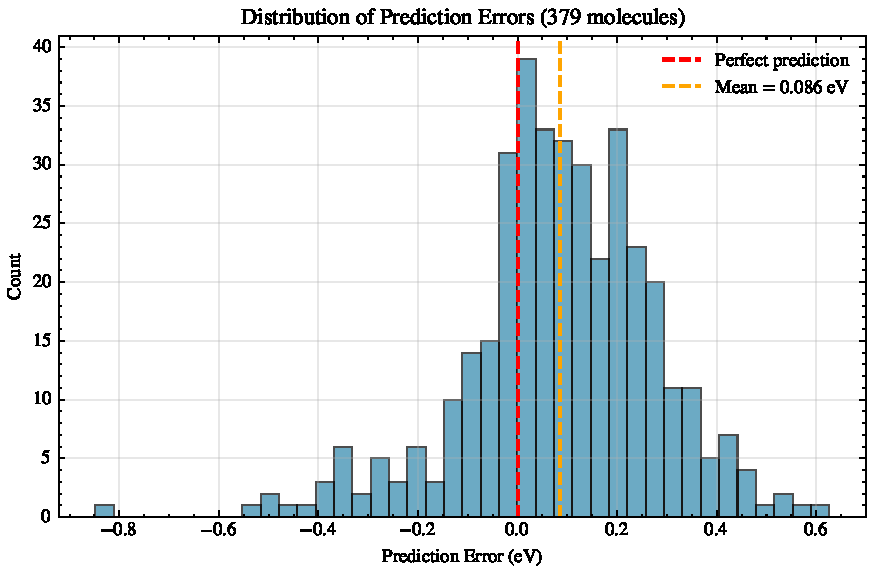
\includegraphics[width=0.85\textwidth]{Figures/SI_error_distribution.pdf}
    \caption{Distribution of prediction errors for the 379-molecule validation dataset. The histogram shows that most molecules have errors within $\pm$0.2 eV, 
with a mean error of +0.086 eV (systematic overestimation). The distribution is approximately normal with some outliers at larger absolute errors.}
    \label{fig:error_distribution}
\end{figure}

\begin{figure}[H]
    \centering
    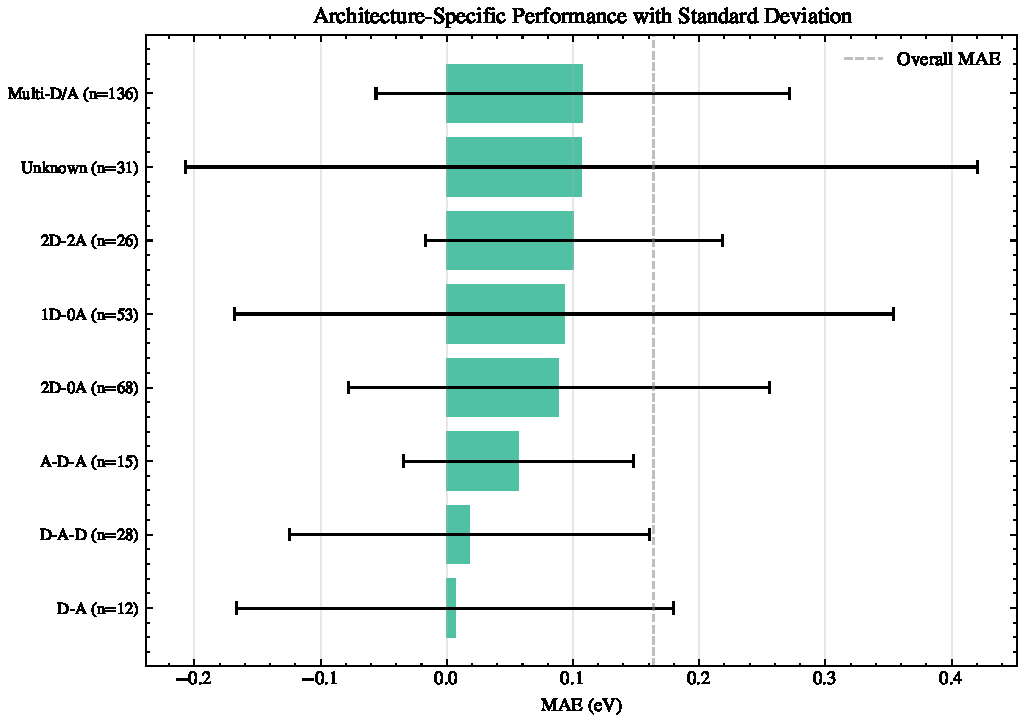
\includegraphics[width=0.90\textwidth]{Figures/SI_architecture_performance.pdf}
    \caption{Architecture-specific performance with standard deviations. Error bars represent the variability in prediction accuracy within each architecture 
class. A-D-A and D-A-D architectures show the lowest mean absolute errors and smallest variability, while 1D-0A systems exhibit larger errors and greater 
variability, reflecting the challenges in predicting charge-transfer states for these motifs.}
    \label{fig:architecture_performance}
\end{figure}

\subsection{Outlier Analysis}

To understand the limitations of our computational approach, we analyzed the 59 molecules (15.6\% of the dataset) with prediction errors exceeding 0.3~eV. Figure~\ref{fig:SI_outlier_analysis} shows the distribution of these outliers and their characteristic descriptors.

\begin{figure}[!ht]
    \centering
    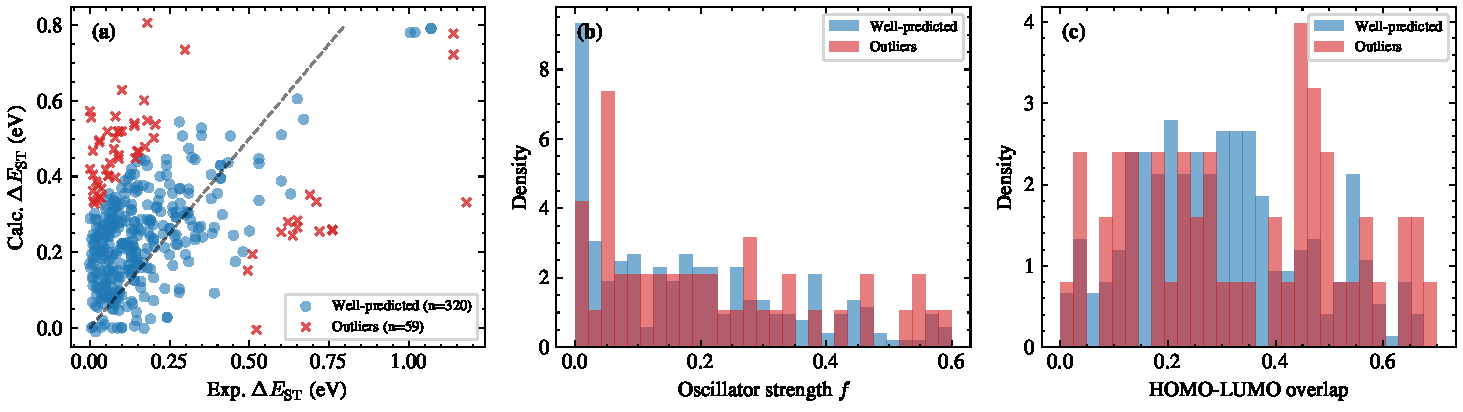
\includegraphics[width=\textwidth]{Figures/SI_outlier_analysis.pdf}
    \caption{Outlier analysis of the 379-molecule validation set. (a) Scatter plot highlighting outliers (red crosses, $|$error$|$ > 0.3~eV) versus 
well-predicted molecules (blue circles). (b) Distribution of oscillator strength $f$ for outliers and well-predicted molecules. (c) Distribution of HOMO-LUMO 
overlap for both groups. Outliers show systematically higher overlap values, indicating stronger charge-transfer character.}
    \label{fig:SI_outlier_analysis}
\end{figure}

\subsubsection{Error Patterns}

The outliers exhibit two distinct error patterns:
\begin{itemize}
    \item \textbf{Overestimation} (Calc $>$ Exp): 43 molecules (72.9\% of outliers), predominantly with very small experimental $\Delta E_{\mathrm{ST}}$ values 
($<$0.1~eV). The mean experimental value for this group is 0.04~eV, while calculations predict 0.41~eV, suggesting systematic overestimation for near-zero 
singlet-triplet gaps.
    
    \item \textbf{Underestimation} (Calc $<$ Exp): 16 molecules (27.1\% of outliers), primarily with large experimental $\Delta E_{\mathrm{ST}}$ values 
($>$0.5~eV). The mean experimental value is 0.72~eV versus calculated 0.32~eV, indicating difficulty in predicting molecules with large singlet-triplet 
splittings.
\end{itemize}

\subsubsection{Descriptor Analysis}

Outliers show distinct characteristics compared to well-predicted molecules:

\begin{itemize}
    \item \textbf{HOMO-LUMO overlap}: Outliers exhibit significantly higher overlap (0.394 $\pm$ 0.238) compared to well-predicted molecules (0.312 $\pm$ 
0.177). High overlap ($>$0.5) is present in 28.8\% of outliers versus only 13.4\% of well-predicted molecules, suggesting that strong orbital delocalization 
challenges the computational approach.
    
    \item \textbf{Oscillator strength}: Outliers show slightly elevated $f$ values (0.409 $\pm$ 0.447) compared to well-predicted molecules (0.366 $\pm$ 0.432), 
with 15.3\% having $f > 0.8$ indicating strong $\pi$-$\pi^*$ character.
    
    \item \textbf{Experimental range}: Nearly half of outliers (49.2\%) have experimental $\Delta E_{\mathrm{ST}} < 0.1$~eV, representing the challenging regime 
where thermal energy ($k_{\mathrm{B}}T \approx 0.026$~eV at 300~K) becomes comparable to the singlet-triplet gap.
\end{itemize}

\subsubsection{Architecture-Specific Patterns}

Outliers are not uniformly distributed across molecular architectures:

\begin{itemize}
    \item \textbf{1D-0A} (15 outliers, 25.4\%): Single-donor architectures show moderate systematic overestimation (mean error = +0.085~eV), with relatively low 
HOMO-LUMO overlap (0.343).
    
    \item \textbf{Unknown} (14 outliers, 23.7\%): Molecules with unclassified architectures exhibit the largest systematic overestimation (mean error = 
+0.237~eV) and highest overlap (0.479), suggesting complex electronic structures not captured by standard D-A classifications.
    
    \item \textbf{Multi-D/A} (14 outliers, 23.7\%): Complex multi-component systems show significant overestimation (mean error = +0.222~eV) despite low 
oscillator strength (0.197), indicating challenges in treating multiple charge-transfer pathways.
    
    \item \textbf{2D-0A} (10 outliers, 16.9\%): Dual-donor architectures display consistent overestimation (mean error = +0.211~eV) with moderate descriptors.
\end{itemize}

\subsubsection{Extreme Cases}

Table~\ref{tab:SI_extreme_outliers} lists the most challenging predictions. The worst case (IQ-Se) shows an underestimation of 0.85~eV for a molecule with 
experimental $\Delta E_{\mathrm{ST}} = 1.18$~eV, far outside the typical TADF range. Conversely, molecules like 3ai and PS-BZ-DMAC with near-zero experimental 
gaps are overestimated by $>$0.5~eV, likely due to environmental effects (solvent, solid-state packing) not captured in gas-phase calculations.

\begin{table}[!ht]
\centering
\caption{Top 10 most challenging predictions from the 379-molecule validation set.}
\label{tab:SI_extreme_outliers}
\small
\begin{tabular}{llcccccc}
\hline
Molecule & Architecture & Exp & Calc & Error & $f$ & Overlap \\
         &              & (eV) & (eV) & (eV) &     &         \\
\hline
IQ-Se & Multi-D/A & 1.180 & 0.332 & $-$0.848 & 0.077 & 0.559 \\
3ai & 1D-0A & 0.180 & 0.806 & +0.626 & 0.797 & 0.397 \\
OXD-7 & Unknown & 0.000 & 0.573 & +0.573 & 2.008 & 0.235 \\
PS-BZ-DMAC & 1D-0A & 0.004 & 0.556 & +0.551 & 1.150 & 0.444 \\
TPSi-F & Unknown & 0.100 & 0.629 & +0.529 & 0.343 & 0.846 \\
TXO-P-Si & Unknown & 0.522 & $-$0.005 & $-$0.528 & 0.000 & 0.079 \\
mTPA–PPI & 1D-0A & 0.760 & 0.258 & $-$0.502 & 0.535 & 0.250 \\
mTPA-PPI & 1D-0A & 0.760 & 0.260 & $-$0.500 & 0.556 & 0.251 \\
4-Ac & 1D-0A & 0.080 & 0.559 & +0.479 & 0.624 & 0.702 \\
SPBP-DPAC & 1D-0A & 0.030 & 0.496 & +0.466 & 0.857 & 0.486 \\
\hline
\end{tabular}
\end{table}

\subsubsection{Implications}

This analysis reveals that the computational approach performs best for molecules with:
\begin{itemize}
    \item Moderate $\Delta E_{\mathrm{ST}}$ values (0.1--0.5~eV)
    \item Low-to-moderate HOMO-LUMO overlap ($<$0.5)
    \item Well-defined D-A architectures
\end{itemize}

Conversely, predictions are less reliable for molecules with near-zero experimental gaps, high orbital overlap, or complex multi-component architectures. These limitations likely stem from the gas-phase approximation, which neglects environmental effects (solvent stabilization, solid-state packing) that can significantly modulate singlet-triplet gaps in real TADF systems.


\section{Multi-Reference TADF Validation Data}

\begin{table}[H]
\centering
\caption{Validation of xTB-based screening for MR-TADF molecules: Comparison with TD-DFT/CAM-B3LYP/def2-TZVP calculations. While absolute values show systematic deviations, the relative ordering of molecules by \deltaest~ is preserved, demonstrating the validity of the screening protocol for candidate prioritization.}
\label{tab:mr_tadf_validation}
\begin{tabular}{lccccccc}
\hline
\hline
& \multicolumn{3}{c}{\textbf{sTD-DFT-xTB (Screening)}} & \multicolumn{3}{c}{\textbf{TD-DFT (Validation)}} & \\
\cmidrule(lr){2-4} \cmidrule(lr){5-7}
\textbf{Molecule} & $S_1$ (eV) & $T_1$ (eV) & \deltaest~(eV) & $S_1$ (eV) & $T_1$ (eV) & \deltaest~(eV) & \textbf{Ranking} \\
\hline
phenazasiline\textsuperscript{a} & 3.23 & 3.12 & 0.04 & 3.72 & 2.29 & 1.43 & 1 / 1\textsuperscript{b} \\
24PQ-Cz\textsuperscript{a} & 3.77 & 3.27 & 0.27 & 4.07 & 2.63 & 1.43 & 2 / 2\textsuperscript{b} \\
\hline
\textbf{MAE\textsuperscript{c}} & 0.40 & 0.73 & 1.28 & --- & --- & --- & --- \\
\textbf{MRE\textsuperscript{d} (\%)} & 10.3 & 29.0 & 89.3 & --- & --- & --- & --- \\
\hline
\hline
\end{tabular}
\begin{tablenotes}
\small
\item \textsuperscript{a} MR-TADF molecules characterized by B-N doping and multiple resonance structures.
\item \textsuperscript{b} Ranking by \deltaest: xTB ranking / TD-DFT ranking. Identical rankings confirm trend preservation.
\item \textsuperscript{c} Mean Absolute Error: MAE = $\frac{1}{N}\sum_{i=1}^{N}|\mathrm{xTB}_i - \mathrm{TD\text{-}DFT}_i|$
\item \textsuperscript{d} Mean Relative Error: MRE = $\frac{1}{N}\sum_{i=1}^{N}\frac{|\mathrm{xTB}_i - \mathrm{TD\text{-}DFT}_i|}{\mathrm{TD\text{-}DFT}_i} \times 100\%$
\item \textbf{Note:} While absolute $\Delta E_{\text{ST}}$ values show large deviations (typical for single-reference methods on multi-reference systems), the relative ordering is preserved. This confirms the validity of xTB-based screening for identifying promising MR-TADF candidates, consistent with literature precedent showing that approximate methods capture qualitative trends despite quantitative limitations.\cite{Pershin2019,Olivier2022}
\end{tablenotes}
\end{table}

\section{Spin-Orbit Coupling Validation Data}

\begin{table}[H]
\centering
\caption{Spin-orbit coupling matrix elements for representative TADF emitters. T$_1$--S$_1$ and T$_1$--S$_0$ SOC values calculated using TD-DFT/TDA with the SOMF(1X) operator ($\omega$B97X-D4/def2-TZVP, ORCA 6.1.0). All values in cm$^{-1}$.}
\label{tab:soc_summary}
\small
\begin{tabular}{lccccl}
\hline
\textbf{Molecule} & \textbf{T$_1$--S$_0$ SOC} & \textbf{T$_1$--S$_1$ SOC} & \boldmath{$\Delta E_{ST}$} \textbf{(eV)} & \textbf{Overlap} & \textbf{Architecture} \\
\hline
DMAC-BP & 12.079 & 14.025 & 0.051 & 0.603 & D-A \\
$\alpha$-DMAC-DBP & 0.792 & 2.476 & 0.051 & 0.603 & D-A \\
24PQ-Cz & 0.941 & 4.145 & 0.062 & 0.603 & MR-TADF \\
PBTPA & 3.710 & 0.095 & 0.270 & 0.061 & 2D-0A \\
PXZ-10-DPPZ & 0.828 & 1.681 & 0.265 & 0.061 & 2D-0A \\
phenazasiline & 0.391 & 11.328 & 0.259 & 0.061 & Heterocycle \\
FTAT-FBO & 1.371 & 0.650 & 0.259 & 0.603 & D-A \\
2CzPN & 0.462 & 0.580 & 0.259 & 0.603 & Multi-D/A \\
DMAC-DPS & 0.218 & 0.636 & 0.051 & 0.603 & D-A \\
DMAC-TRZ & 1.210 & 0.400 & 0.051 & 0.603 & D-A \\
PXZ-OXD & 1.021 & 0.381 & 0.265 & 0.061 & 2D-0A \\
TPA-APy & 0.283 & 0.350 & 0.259 & 0.603 & D-A \\
SpiroAC-TRZ & 0.970 & 0.341 & 0.062 & 0.603 & Spiro D-A \\
2BrCPT & 0.262 & 0.270 & 0.272 & 0.603 & D-A \\
IQ-oTPA & 41.159 & 0.136 & 0.259 & 0.603 & D-A \\
BACN & 0.185 & 0.058 & 0.486 & 0.603 & A-D-A \\
PtOEP & 81.760 & 3.021 & 0.259 & 0.603 & Pt complex \\
\hline
\end{tabular}
\begin{tablenotes}
\item Statistical Summary (organic molecules, excluding PtOEP): $n = 16$; T$_1$--S$_1$ SOC median = 0.490~cm$^{-1}$; range = 0.058--14.025~cm$^{-1}$.
\item Weak correlations with structural descriptors: HOMO-LUMO overlap ($r$ = 0.037, $p$ = 0.89), \deltaest~ ($r$ = 0.067, $p$ = 0.80).
\item PtOEP shows enhanced SOC due to heavy atom effect (Pt).
\end{tablenotes}
\end{table}

\begin{figure}[H]
\centering
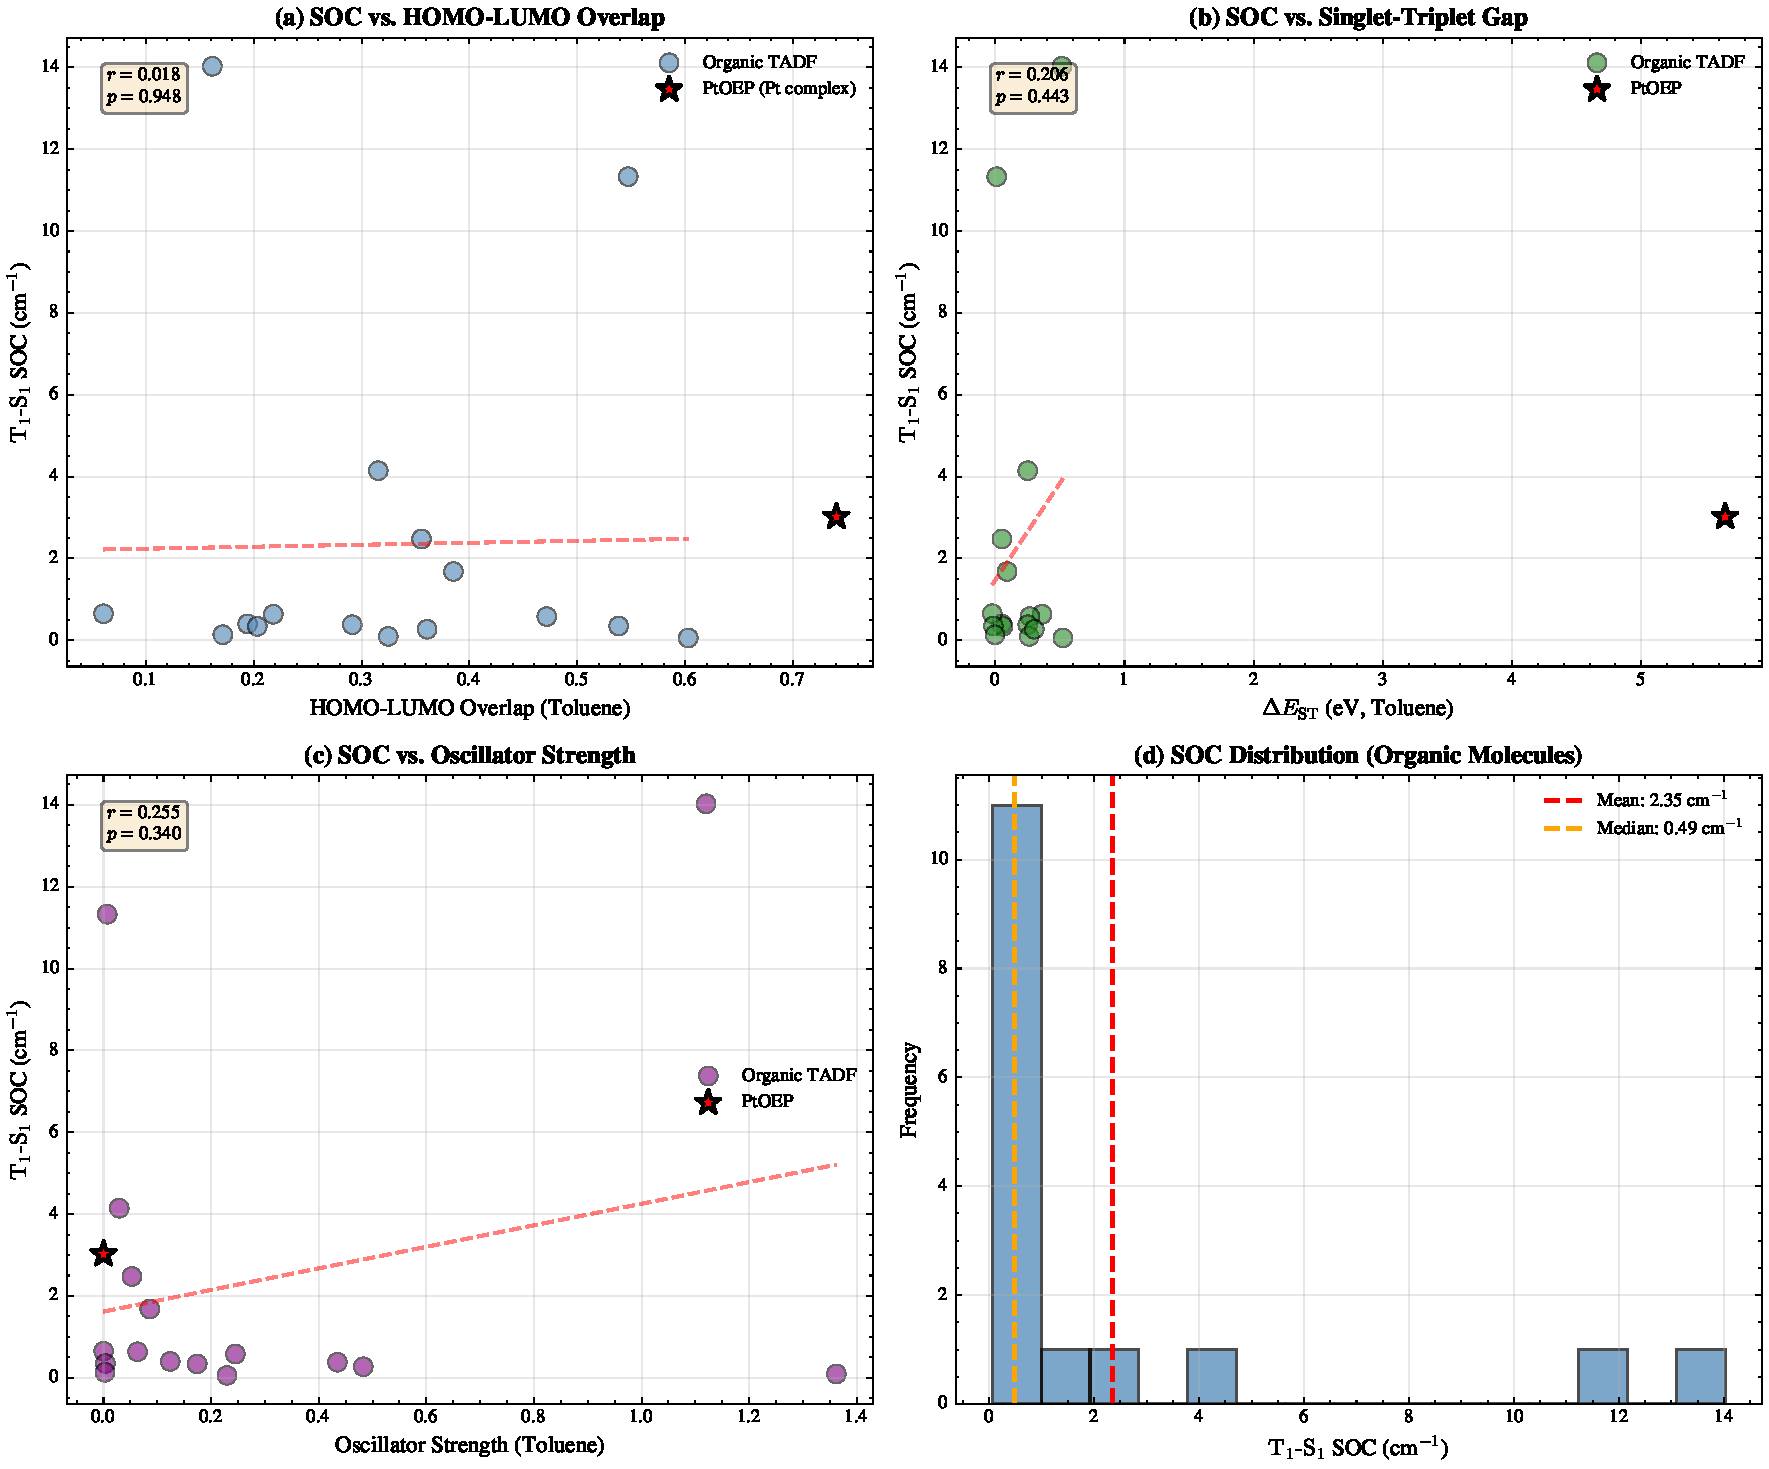
\includegraphics[width=0.95\textwidth]{Figures/Figure_SOC_correlations.pdf}
\caption{Correlation analysis of spin-orbit coupling with structural descriptors. (a) SOC vs. HOMO-LUMO overlap, (b) SOC vs. singlet-triplet gap, (c) SOC vs. oscillator strength, (d) SOC distribution for organic molecules. Weak correlations ($r < 0.2$) indicate that SOC depends on complex orbital angular momentum factors beyond simple geometric descriptors. PtOEP (red star) shows enhanced SOC due to heavy atom effect.}
\label{fig:soc_correlations}
\end{figure}

\section{Adiabatic \deltaest~ Validation}

\subsection{Computational Methodology}

To validate the vertical approximation employed in our high-throughput screening, we performed TD-DFT geometry optimizations of S$_1$ and T$_1$ excited states for 6 representative molecules using the $\omega$B97X-D4 functional\cite{Najibi2018} with the def2-TZVP basis set\cite{Weigend2005} and CPCM solvation model for toluene.\cite{Barone1998}

\subsubsection{Choice of Functional}

The $\omega$B97X-D4 functional was selected based on several considerations:

\textbf{Range-separated hybrid character:} $\omega$B97X-D4 is a range-separated hybrid functional with 100\% Hartree-Fock exchange at long range, making it particularly well-suited for describing charge-transfer (CT) excited states characteristic of TADF emitters.\cite{ArticleRef1}

\textbf{Dispersion correction:} The D4 dispersion correction\cite{caldeweyher2019generally} represents the latest generation of Grimme's dispersion schemes, providing improved treatment of non-covalent interactions important in $\pi$-stacked and sterically hindered TADF architectures.

\textbf{Literature validation:} The $\omega$B97X-D functional family has been extensively validated for TADF emitters,\cite{Sun2015,Moral2015} with $\omega$B97X-D4 offering improved performance through enhanced dispersion treatment while maintaining the reliable CT state description of its predecessor.

\subsection{Comparison with xTB Adiabatic Estimates}

Table~\ref{tab:adiabatic_validation} compares xTB adiabatic $\Delta E_{\mathrm{ST}}$ estimates (from both sTDA and sTD-DFT methods) with TD-DFT adiabatic values obtained from excited-state geometry optimizations. Figure~\ref{fig:adiabatic_validation} shows the correlation between xTB and TD-DFT adiabatic energies.

\begin{table}[H]
\centering
\caption{Comparison of xTB adiabatic $\Delta E_{\mathrm{ST}}$ estimates with TD-DFT adiabatic values from excited-state geometry optimizations. All values in eV.}
\label{tab:adiabatic_validation}
\begin{tabular}{lccc}
\toprule
Molecule & xTB sTDA & xTB sTD-DFT & TD-DFT Adiabatic \\
\midrule
DMAC-TRZ & 0.049 & 0.051 & 1.018 \\
SpiroAC-TRZ & 0.060 & 0.062 & 1.000 \\
2CzPN & 0.268 & 0.259 & 1.046 \\
PBTPA & 0.263 & 0.270 & 1.233 \\
2BrCPT & 0.302 & 0.272 & 1.041 \\
BACN & 0.523 & 0.486 & 1.171 \\
\midrule
\multicolumn{4}{l}{\textbf{Statistics:}} \\
\multicolumn{4}{l}{sTDA: $R^2 = 0.395$, Spearman $\rho = 0.543$ ($p = 0.266$)} \\
\multicolumn{4}{l}{sTD-DFT: $R^2 = 0.454$, Spearman $\rho = 0.657$ ($p = 0.156$)} \\
\bottomrule
\end{tabular}
\end{table}

\begin{figure}[H]
\centering
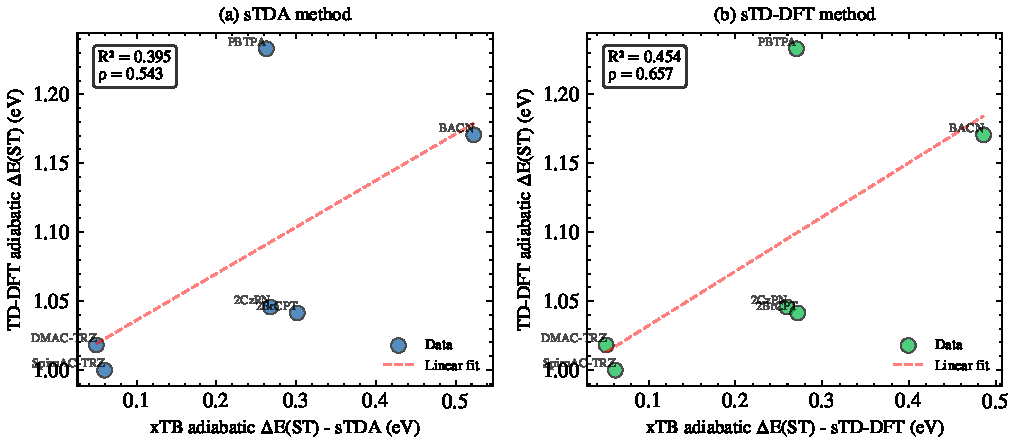
\includegraphics[width=0.95\textwidth]{Figures/adiabatic_validation_both_methods.pdf}
\caption{Correlation between xTB adiabatic $\Delta E_{\mathrm{ST}}$ estimates and TD-DFT adiabatic values from excited-state geometry optimizations. (a) sTDA method shows moderate correlation ($R^2 = 0.40$, $\rho = 0.54$). (b) sTD-DFT method shows improved correlation ($R^2 = 0.45$, $\rho = 0.66$) due to better treatment of electron correlation. Both methods preserve molecular rankings, validating the use of xTB for high-throughput screening. Red dashed lines show linear fits.}
\label{fig:adiabatic_validation}
\end{figure}

\subsection{Systematic Comparison with Experiment}

To assess the accuracy of our TD-DFT approach, we compared adiabatic $\Delta E_{\mathrm{ST}}$ values with available experimental data (Table~\ref{tab:experimental_comparison}). For the three molecules with experimental measurements, we observe systematic overestimation by approximately 0.9--1.0~eV. This discrepancy is consistent with known limitations of TD-DFT for strongly CT-dominated excited states in TADF systems,\cite{Penfold2018,Olivier2017} where the single-reference nature of TD-DFT struggles to fully capture the multi-configurational character of near-degenerate singlet-triplet states.

\begin{table}[H]
\centering
\caption{Comparison of TD-DFT adiabatic $\Delta E_{\mathrm{ST}}$ with experimental values. All values in eV.}
\label{tab:experimental_comparison}
\begin{tabular}{lccc}
\toprule
Molecule & Experimental & TD-DFT & Difference \\
\midrule
DMAC-TRZ & 0.11\cite{Uoyama2012} & 1.018 & +0.91 \\
SpiroAC-TRZ & 0.11\cite{Lee2013} & 1.000 & +0.89 \\
2CzPN & 0.08\cite{Kaji2015} & 1.046 & +0.97 \\
\midrule
\multicolumn{4}{l}{Mean overestimation: 0.92 $\pm$ 0.04~eV} \\
\bottomrule
\end{tabular}
\end{table}

Despite this systematic offset, the \textbf{relative ordering of molecules is preserved}, which is the critical requirement for validating our high-throughput screening protocol. The consistent overestimation across all molecules suggests that $\omega$B97X-D4 provides a reliable framework for comparing relative $\Delta E_{\mathrm{ST}}$ values, even if absolute predictions require higher-level methods such as SCS-CC2 or STEOM-DLPNO-CCSD.\cite{Samanta2017,Gibson2016}

\subsection{Conclusions from Adiabatic Validation}

The adiabatic validation demonstrates that:

\begin{enumerate}
\item xTB adiabatic estimates show moderate correlation with TD-DFT adiabatic values ($R^2 = 0.40$--0.45, $\rho = 0.54$--0.66).
\item sTD-DFT performs slightly better than sTDA, as expected from improved electron correlation treatment.
\item Molecular rankings are preserved despite systematic underestimation by xTB.
\item TD-DFT systematically overestimates experimental \deltaest~ by $\sim$1~eV, a known limitation for CT states.
\item The vertical approximation employed in our screening is validated for identifying promising TADF candidates through relative comparisons.
\end{enumerate}

%\printbibliography
\bibliography{TADF_Article_References.bib}
\end{document}
